


\newpage

\section{Clústering avançat} 

En aquesta secció s'exploraran diferents tècniques avançades de clustering alhora que s'analitzaran i es compararan els resultats obtinguts. Cal mencionar en tots que els objectius de la creació de classes pot resultar diferent sobretot segons el mètode utilitza ja que, per exemple, en el \textit{K-modes} tan sols volem formar clústers per variables categòriques o en el \textit{time series clustering} volem agrupar instàncies de cançons segons una sola variable al llarg del temps.

\subsection{Clústering jeràrquic} \label{section:clustering_jerarquic3}

El clustering jeràrquic és un mètode d'agrupament de dades que no requereix donar-li el nombre de grups com a paràmetre, ja que es representa amb dendrograma (que mostra la relació de similitud entre els elements) i a partir d'allà es pot escollir la k. Aquest mètode ja es va explorar el quatrimetre passat.

En aquest apartat es fa un clústering jeràrquic però afegint les noves variables creades durant el preprocessament de les dades per veure de quina manera aquestes variables afecten a aquest agrupament. A l'agrupament les variables que no han estat incluides han estat week\_index i day\_release ja que s'ha considerat que es feient millor els clústers sense afegir-les. Tampoc s'han incluit les variables track\_id, track\_name, album\_name i artist\_name. 

% Foto del dendrograma sense pintar
\begin{figure}[H]
    \centering
    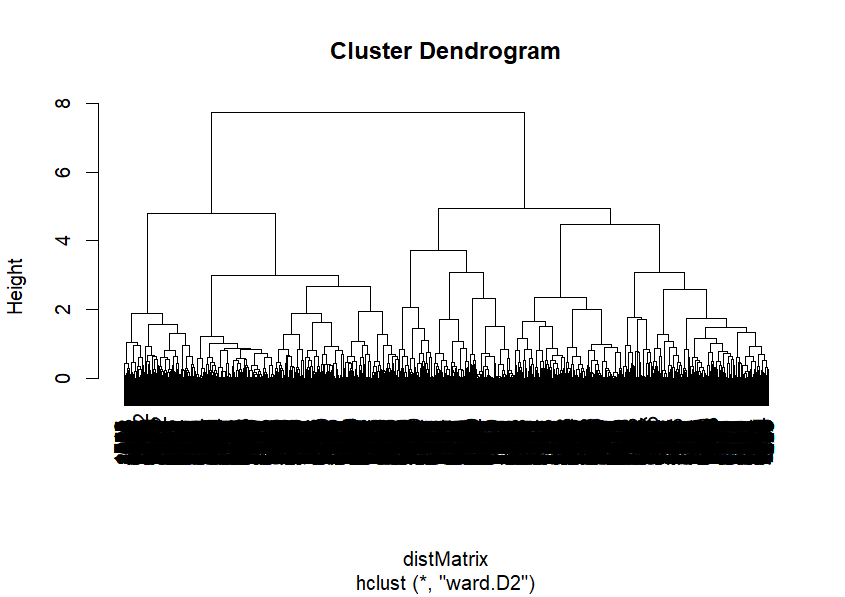
\includegraphics[width=0.8\textwidth]{Images/4_clustering/herarchical/dendogram.png}
    \caption{Dendrograma del clustering jeràrquic}
    \label{fig:dendogram}
\end{figure}

Observant el dendrograma, podem veure que es podria dividir entre dues classes, però per fer el profiling considerem que és millor agafar més classes. L'han passat vam triar 4 clústers, però en el cas d'ara ens quedarien les classes poc balancejades. Per això, triem 5 clústers.  

Amb el dendrograma resultant, es divideixen els 5 clústers de la següent manera: 

\begin{figure}[H]
    \centering
    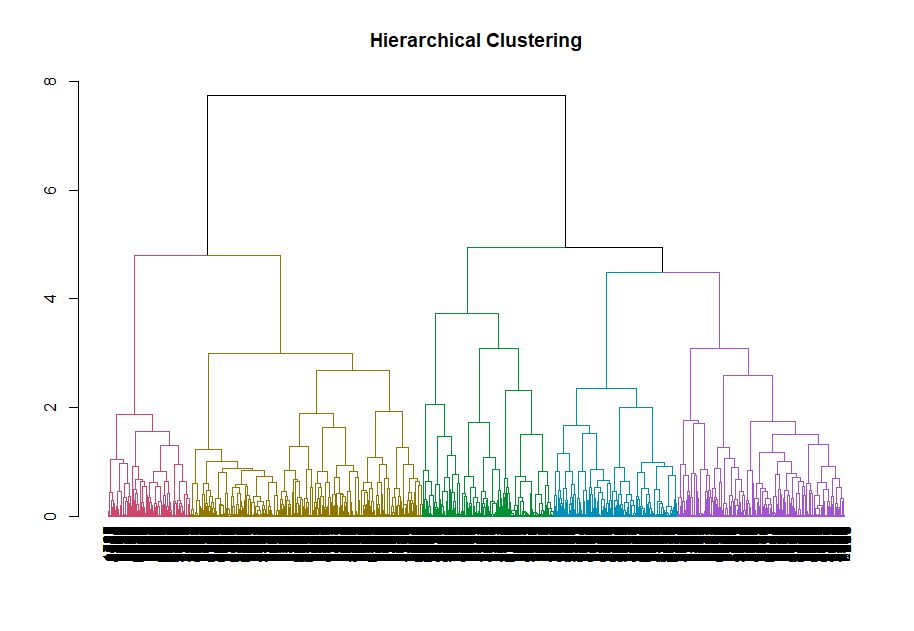
\includegraphics[width=0.8\textwidth]{Images/4_clustering/herarchical/hierarchical_dendogram_colors2.png}
    \caption{Dendrograma del clustering jeràrquic després de crear els clústers}
    \label{fig:hierarchical_dendogram_colors2}
\end{figure}

Abans de realitzar el profiling del clústering jeràrquic, s'ha realitzat un PCA per poder observar els clusters que s'han identificat en el clústering jeràrquic en les dos primeres components principals.

\begin{figure}[H]
    \centering
    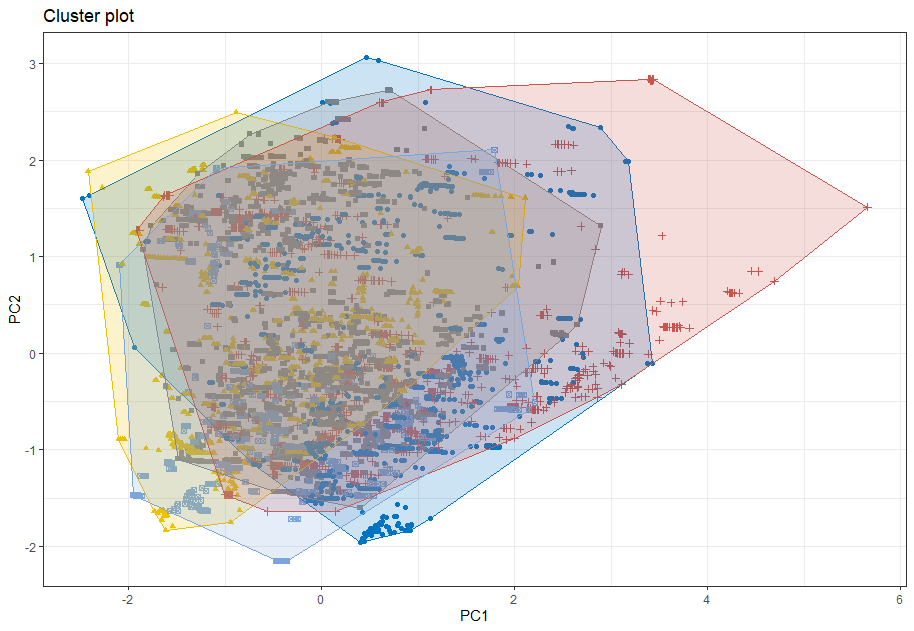
\includegraphics[width=0.7\textwidth]{Images/4_clustering/herarchical/pca_hierarchical.png}
    \caption{Resultats del clústering jerarquic}
    \label{fig:pca_hierarchical}
\end{figure}

Com es pot observar, tenim 5 clústers, uns semblen més dispersos i altres més densos indicant variacions en la cohesió interna dels grups. Tot i així, és important recalcar que les dos primeres components no capturen una gran informació de les dades (17\% el primer component i 14\% el segon).

Encara que no es pot observar una clara divisió dels clústers degut al baix percentatge de variància explicada en les dos primeres components, amb  el profiling que s'ha realitzat posteriorment, s'examinarà les dades en la seva totalitat i les característiques de cada clúster.   

La mida dels clústers finals és de:
\begin{table}[H]
\centering
\begin{tabular}{|c|c|c|c|c|}
\hline
1    & 2    & 3   & 4   & 5 \\ \hline
1574 & 1997 & 2785 & 1489  & 990  \\ \hline
\end{tabular}
\caption{Resultat del clústering jerarquic}
\label{tab:clustering_results}
\end{table}

Es pot veure que l'últim clúster té una mida més petita que la resta, tot i així, la mida de tots els clústers és bastant similar.

\subsection{K-modes}

El K-modes és un algoritme de clustering i és una extensió del k-means, un algoritme que ja hem treballat en aquesta assignatura. L'algorisme fa bàsicament el mateix però en comptes d'utilitzar dades numèriques, utilitza exclusivament dades categòriques. En el nostre cas hem seleccionat totes les variables categòriques que ja teniem ("pop","hip\_hop", "collab","rank\_group"...) i a més les noves variables afegides durant el preprocessament ("gender", "is\_group", "nationality",\"city"). La variable lyrics no s'ha inclòs en el clustering.

Divideix les dades en un nombre k de grups basant-se en la similitud entre ells. La k, com al k-means, és un hiperparàmetre que hem de triar nosaltres. Per veure la similitud de les dades, en comptes d'utilitzar la distància euclidiana, utilitzem una mesura de disimilitud per a dades categòriques.

Utilitzant el paquet klaR en R, hem fet servir kmodes() donant-li el hiperparàmetre k = 4. Com no es poden utilitzar mètriques de validació per les variables categòriques, s'ha triat la k no agafant un nombre molt gran, i a partir del clustering jeràrquic que vam fer l'any passat. 

Un cop s'ha realitzat el K-Modes, s'ha realitzat un Anàlisi dels Components Principals (ACP) per visualitzar la distribució dels clústers respecte les variables numèriques. No s'ha observat una classificació clara de les variables numèriques en els clústers realitzats amb les variables categòriques. Tot i així, en la cinquena i sisena dimensió (8,5\% i 6\% de variància explicada respectivament) si que s'observa una petita separació entre clústers.  \\

\begin{figure}[H]
    \centering
    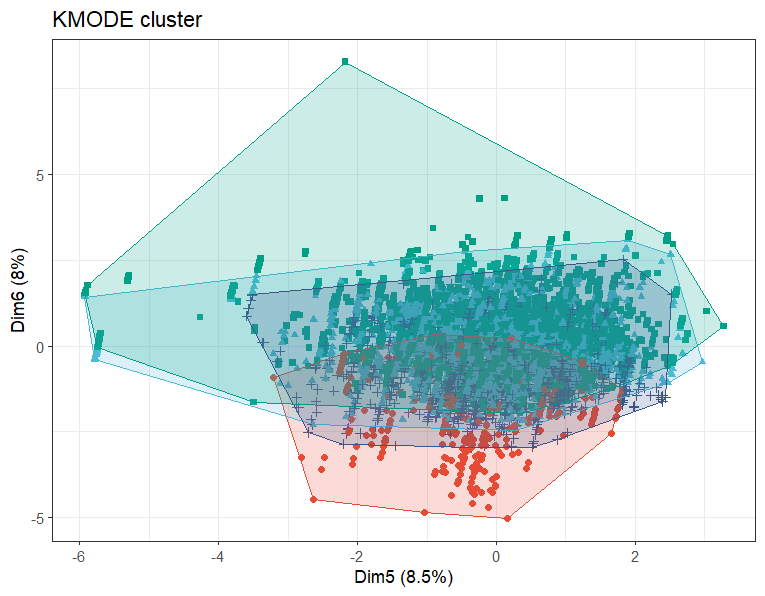
\includegraphics[width=0.7\textwidth]{Images/4_clustering/KMODES/kmodes1.png}
    \caption{Resultats del K-Modes en la 5ª i 6ª dimensió}
    \label{fig:kmodes1}
\end{figure}

La dimensió 5 està relacionada amb l'speechines i el tempo d'una cançó i la dimensió 6 està més relacionada amb el número d'artistes, la duració i la danceability d'una cançó. Per tant, es podria indicar que el K-Means divideix els clústers segons aquestes característiques. Tot i així, cal recalcar que aquestes dimensions només expliquen un 16\% de la variància total de les dades, per tant, caldria fer el profiling per poder afirmar aquesta conclusió.

\begin{figure}[H]
    \centering
    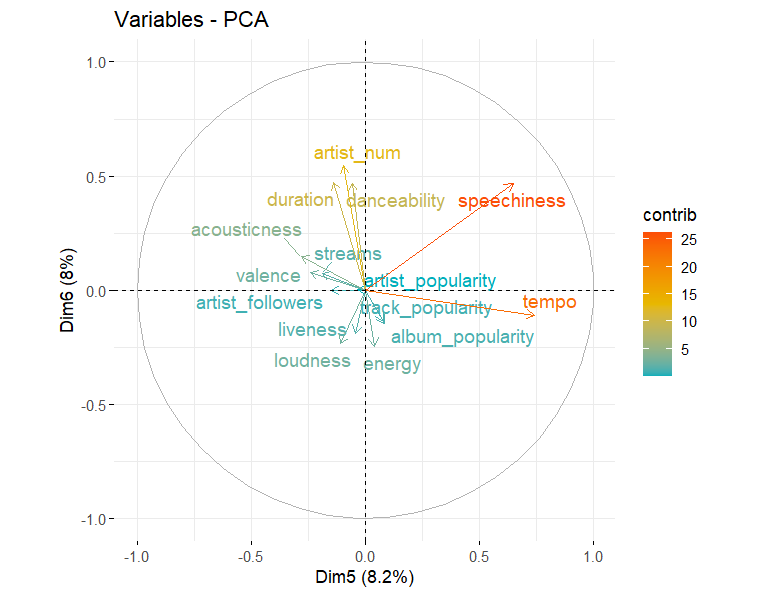
\includegraphics[width=0.7\textwidth]{Images/4_clustering/KMODES/kmodes2.png}
    \caption{Variables i la seva contribució en el 5é i 6é components principals}
    \label{fig:kmodes2}
\end{figure}

Un cop fet ja s'ha experimentat amb el k-means i amb el k-modas, s'ha trobat interessant  fer ús del k-prototypes. Aquesta és una tècnica que barreja les variables numèriques i categòriques. S'ha utilitzat la funció kproto() de clustMixType per fer el clustering. Com amb el k-means, basant-nos en els resultats de l'últim agrupament, s'ha utilitzat el número de clústers k=4. També s'han afegit més paràmetres. El paràmetre lambda s'encarrega d'equilibrar la importància entre els dos tipus de variales, també hem posat un màxim d'iteracions i el nombre d'ejecucions a fer amb diferents centroides inicials (nstart). 

\subsection{CURE}
Clustering Using REpresentatives (\cite{guha_1998_cure}) és una tècnica avançada de clústering centrada en millorar el rendiment d’aquest tipus d’algorismes per bases de dades especialment grans. Es basa en el concepte de trobar uns punts representatius inicials i realitzar el clústering amb aquests. Un cop es troben uns centroides adequats, es calculen les distàncies de la resta dels punts a aquests i s’escull el millor.

S’ha escollit realitzar-lo usant tant les variables numèriques com algunes categòriques (gèneres...). Per tal de poder combinar aquestes variables mixtes, les categòriques s’han transformat prèviament en one-hot-encoding. A més, per evitar problemes amb les magnituds (algunes numèriques tenien valors entre 0 i 1 mentres que d’altres arribaven als milions), les variables numèriques s’han escalat usant la funció scale de R.

\begin{figure}[H]
    \centering
    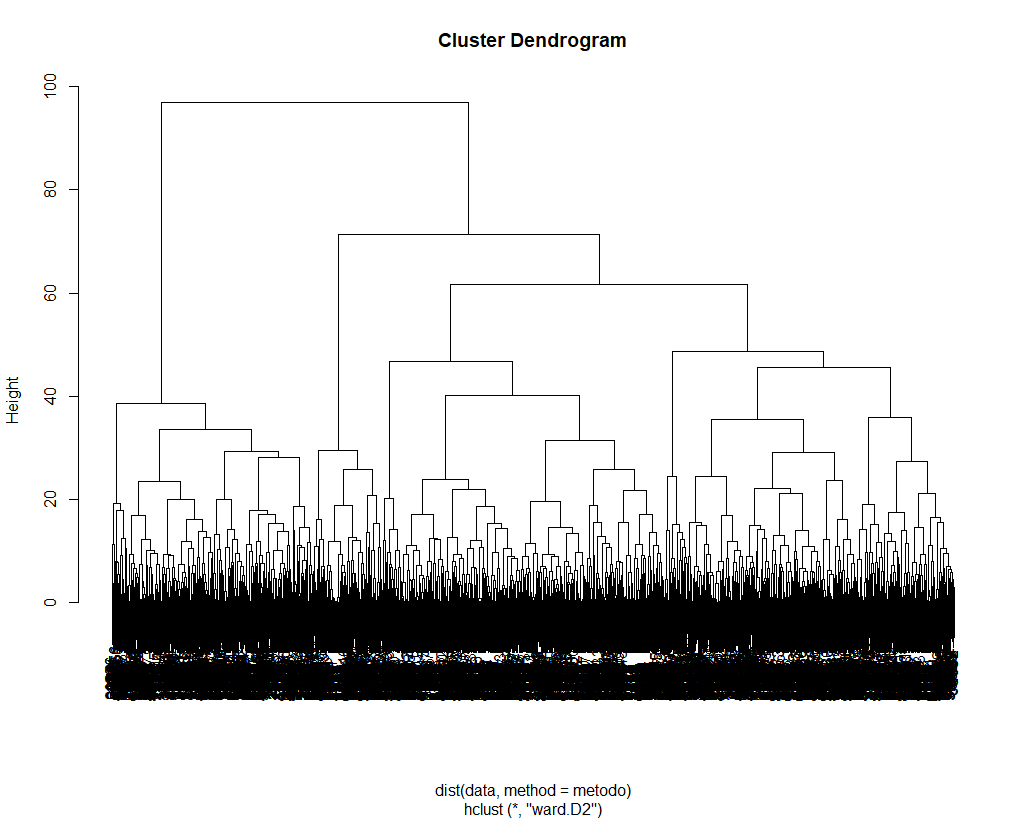
\includegraphics[width=0.8\textwidth]{Images/4_clustering/CURE/curedendrogram.png}
    \caption{Dendrograma de les dades usades pel CURE (jeràrquic, amb ward D2)}
    \label{fig:CURE_dend}
\end{figure}

La distància usada ha estat la euclidiana, ja que després d’aquest petit processat de les dades es podia utilitzar. Amb un  clústering jeràrquic inicial s’ha observat que un bon punt de tall era 4 observant la figura \ref{fig:CURE_dend}, i per tant s’ha escollit aquesta k. La r escollida, és a dir, el percentatge de representatius, ha estat 0.25.

Els 4 clústers dels representatius han quedat amb el següent nombre de cançons en cada un (taula \ref{tab:CURE_taularep}):

\begin{table}[H]
\centering
\begin{tabular}{lllll}
\cline{1-4}
\multicolumn{1}{|c|}{1}   & \multicolumn{1}{c|}{2}   & \multicolumn{1}{c|}{3}    & \multicolumn{1}{c|}{4}   &  \\ \cline{1-4}
\multicolumn{1}{|c|}{653} & \multicolumn{1}{c|}{654} & \multicolumn{1}{c|}{1211} & \multicolumn{1}{c|}{133} &  \\ \cline{1-4}
                          &                          &                           &                          &  \\
                          &                          &                           &                          & 
\end{tabular}
\caption{Resultat del clústering dels representatius}
\label{tab:CURE_taularep}
\end{table}

A partir d’aquests, es poden assignar clústers a la resta de dades. El resultat es pot observar a \ref{tab:CURE_taulanorep}.

\begin{table}[H]
\centering
\begin{tabular}{lllll}
\cline{1-4}
\multicolumn{1}{|c|}{1}    & \multicolumn{1}{c|}{2}    & \multicolumn{1}{c|}{3}   & \multicolumn{1}{c|}{4}   &  \\ \cline{1-4}
\multicolumn{1}{|c|}{3266} & \multicolumn{1}{c|}{1939} & \multicolumn{1}{c|}{670} & \multicolumn{1}{c|}{309} &  \\ \cline{1-4}
                           &                           &                          &                          &  \\
                           &                           &                          &                          & 
\end{tabular}
\caption{Resultat del clústering dels no representatius}
\label{tab:CURE_taulanorep}
\end{table}

Observem com han quedat lleugerament desbalancejats. Se’ns presenta un grup 1 amb moltes de les instàncies, seguit d'un grup 2 que també en té moltes. D'altra banda, els clústers 3 i 4 tenen pocs elements (tot i que el 3 té molts representatius). Els resultats d'aquest clústering es poden visualitzar usant les dues primeres dimensions del PCA, com es pot observar a la figura \ref{fig:CURE_res}.

\begin{figure}[H]
    \centering
    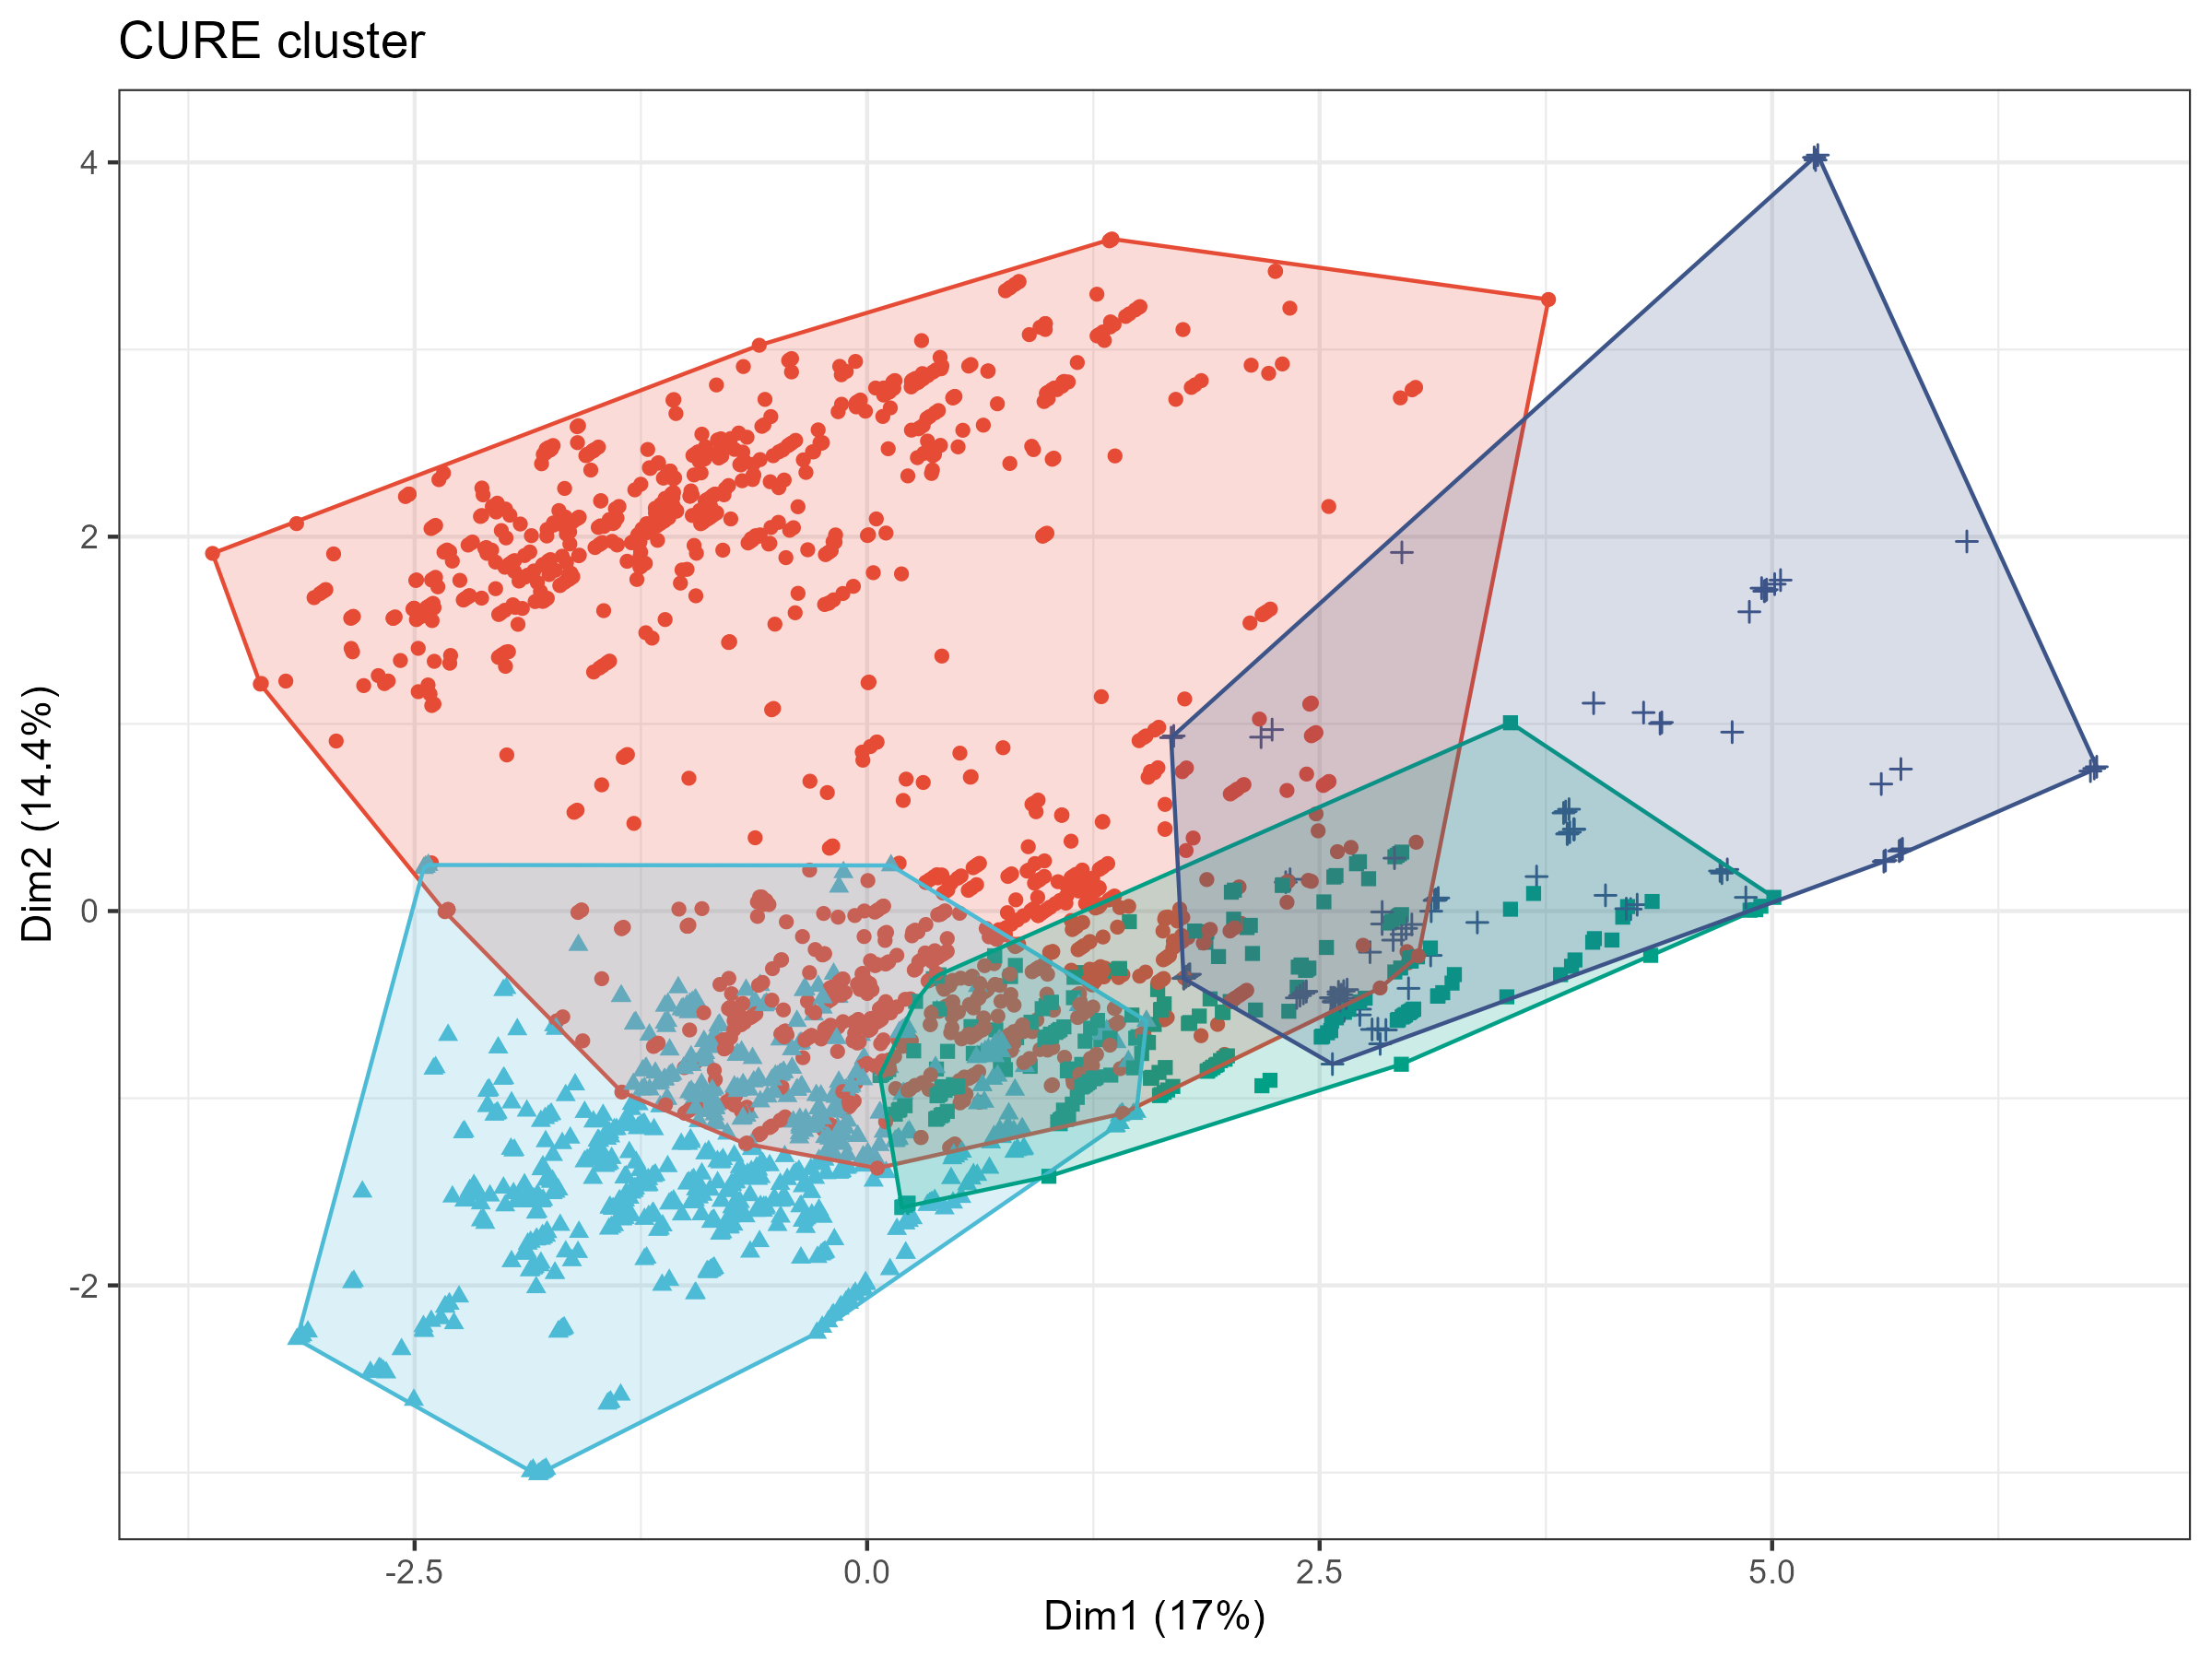
\includegraphics[width=0.8\textwidth]{Images/4_clustering/CURE/cure.png}
    \caption{Resultats del clústering usant CURE (4,0.15)}
    \label{fig:CURE_res}
\end{figure}

S'observa un gran clúster vermell, corresponent probablement al clúster 1. Aquest ocupa un núvol de punts situat a l'espai superior, així com la part central del núvol inferior. Amb valors negatius tant de la primera com de la segona dimensió trobem el clúster blau clar, corresponent al número 2, que és el segon més gran. Finalment, el clúster verd es situa al centre del núvol inferior, amb valors de la dimensió 2 bastant baixos, i el clúster 4, de color blau fosc, és el que engloba els punts amb valors més alts de la dimensió 1.

\subsection{DBSCAN}

El DBSCAN (\cite{dbscan}) és una tècnica de clústering basada en densitat. Per tal de poder observar millor com es reparteixen les nostres dades en aquest aspecte, el primer pas realitzat ha sigut un anàlisi dels components principals (PCA) (figura \ref{fig:DBSCAN_pca}). Aquest, a diferència de l'any passat, no ha estat realitzat en profunditat: tan sols ha estat usat com a tècnica de visualització de dades.

\begin{figure}[H]
    \centering
    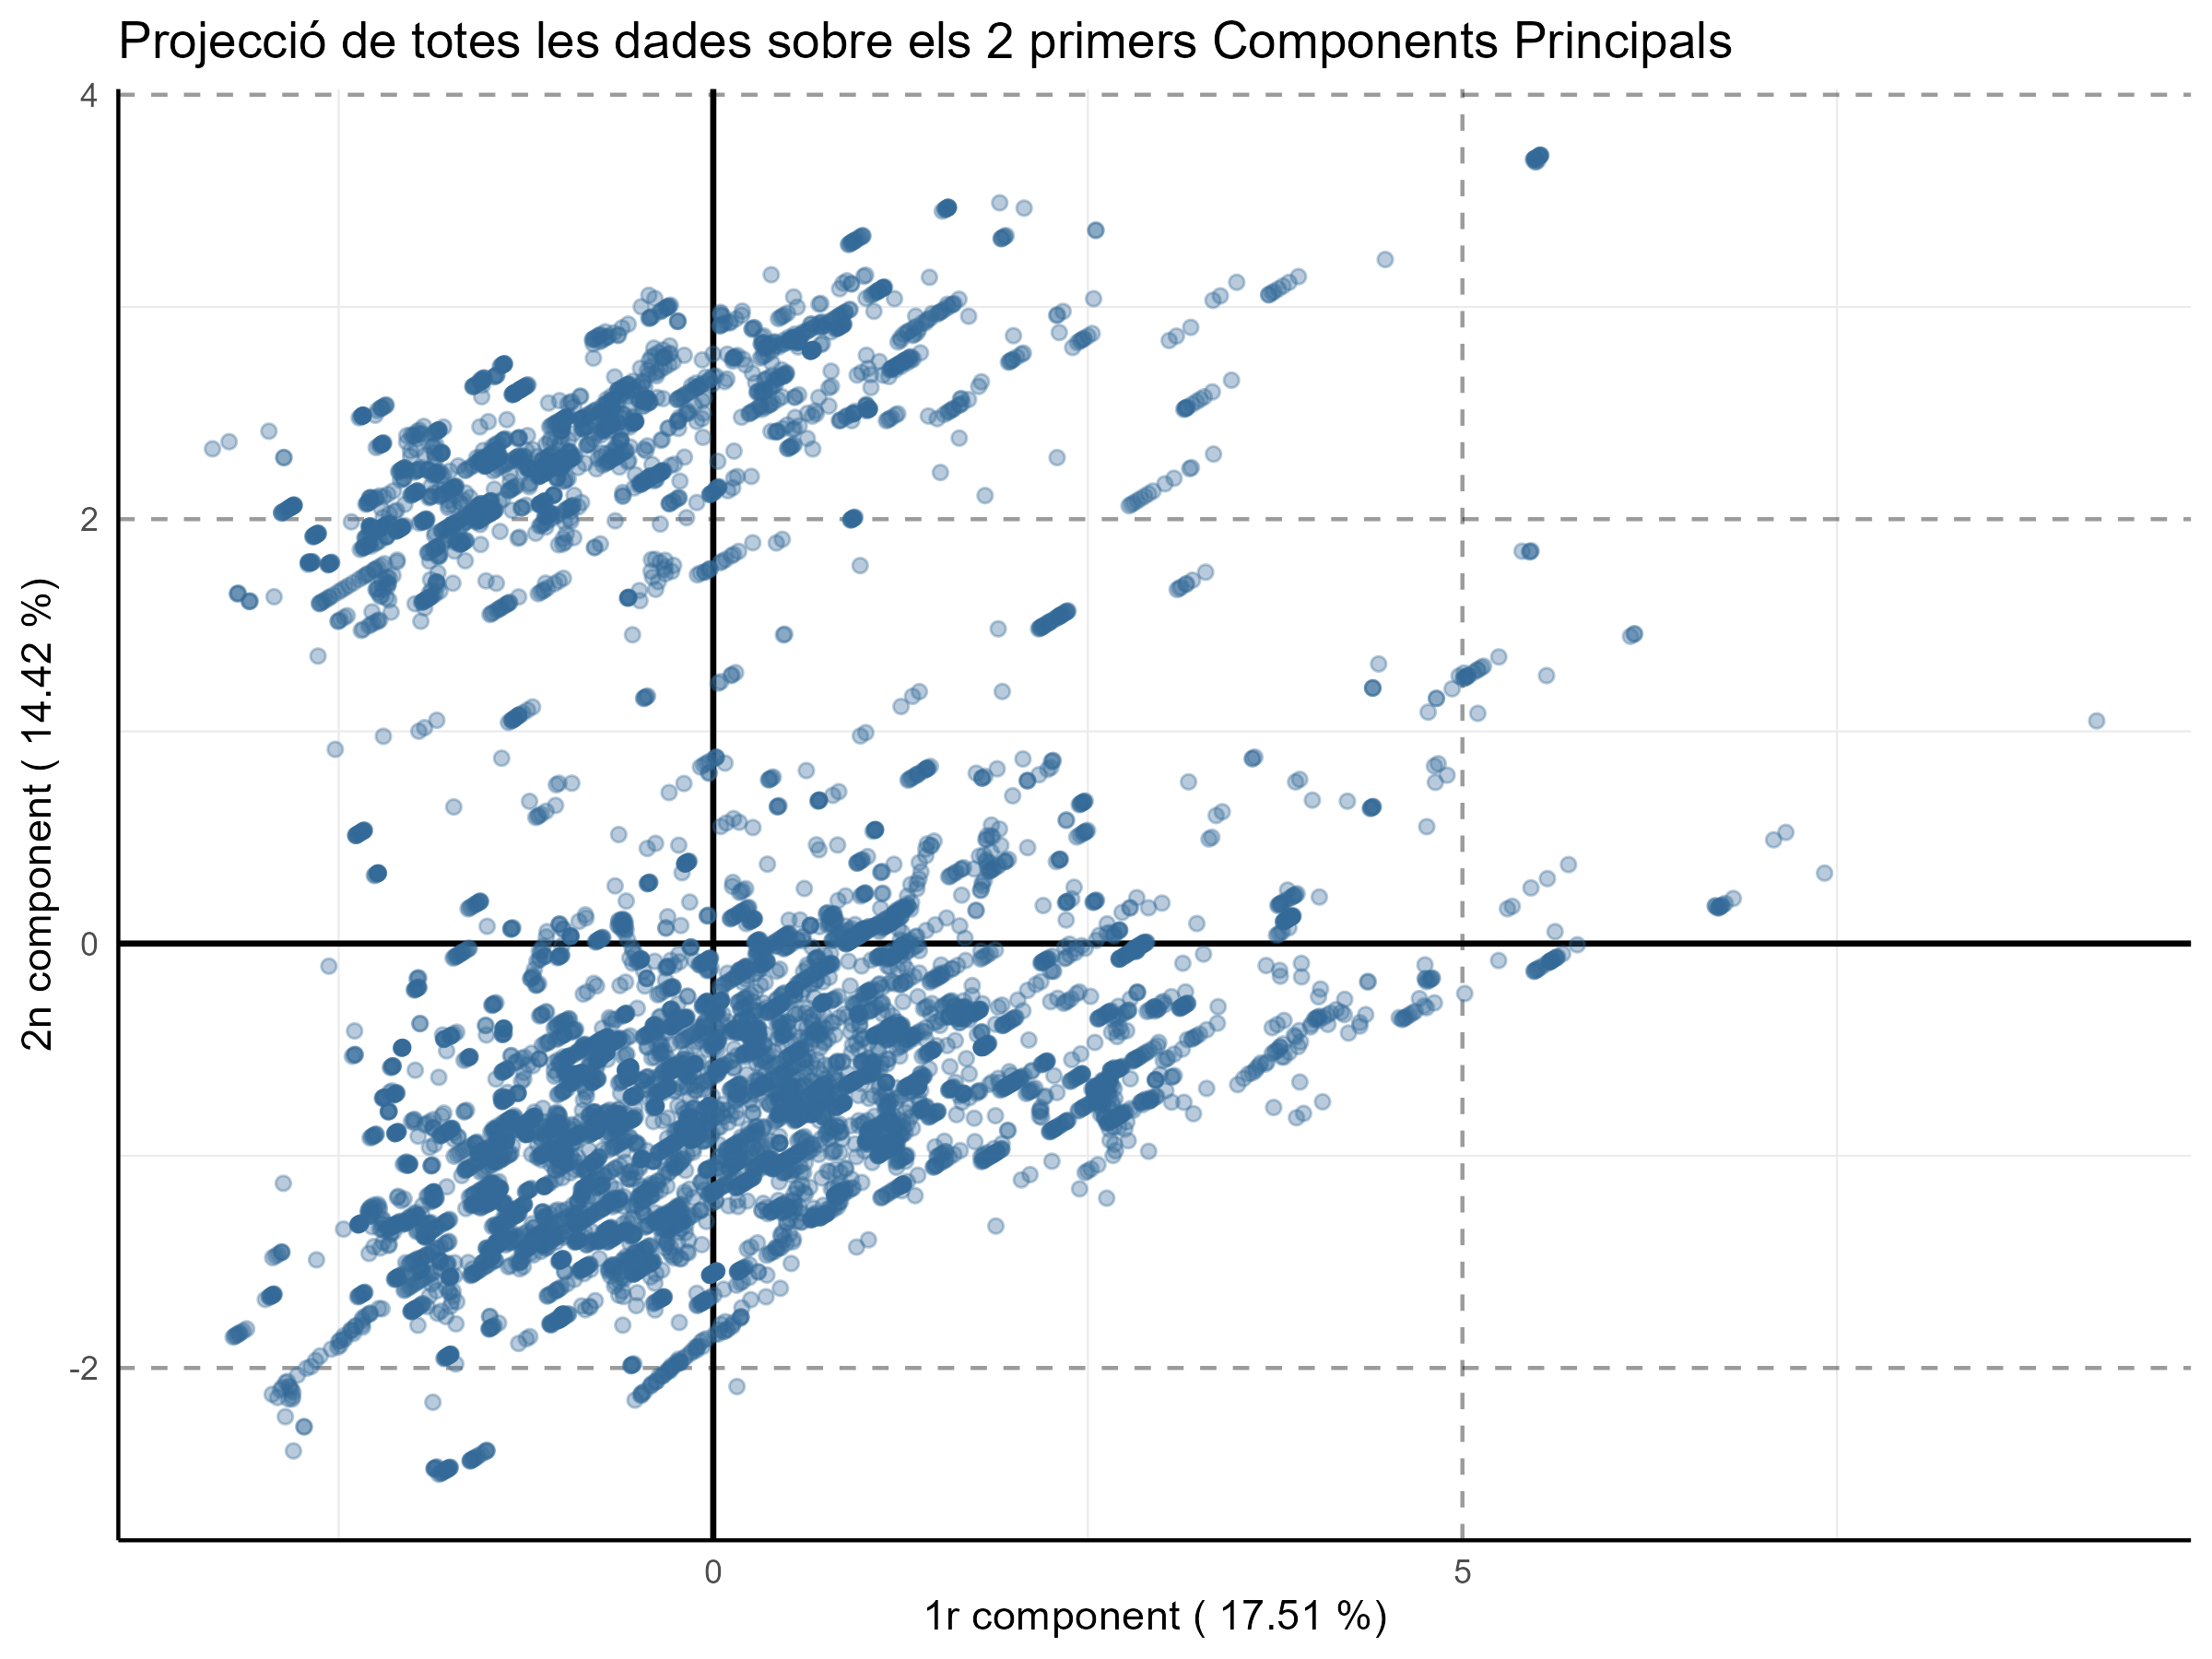
\includegraphics[width=0.8\textwidth]{Images/4_clustering/DBSCAN/dbscanpca.png}
    \caption{Dades descomposades en els dos primers components principals}
    \label{fig:DBSCAN_pca}
\end{figure}

A simple vista, basant-nos en les dues components principals, observem dos grans grups: un amb valors negatius de la segona component i un altre amb valors positius. Analitzant les variables que influeixen en aquests components (figura \ref{fig:DBSCAN_pca_contrib}), sembla ser que el grup inferior conté cançons més populars, mentres que l'altre conté cançons més antigues i per tant menys populars (Dimensió 2). La dimensió 1 ens indica com d'acústica o trista és la cançó: valors negatius indiquen cançó positiva, amb energia i forta (potent) mentre que valors positius indiquen una major \textit{acousticness}.

\begin{figure}[H]
    \centering
    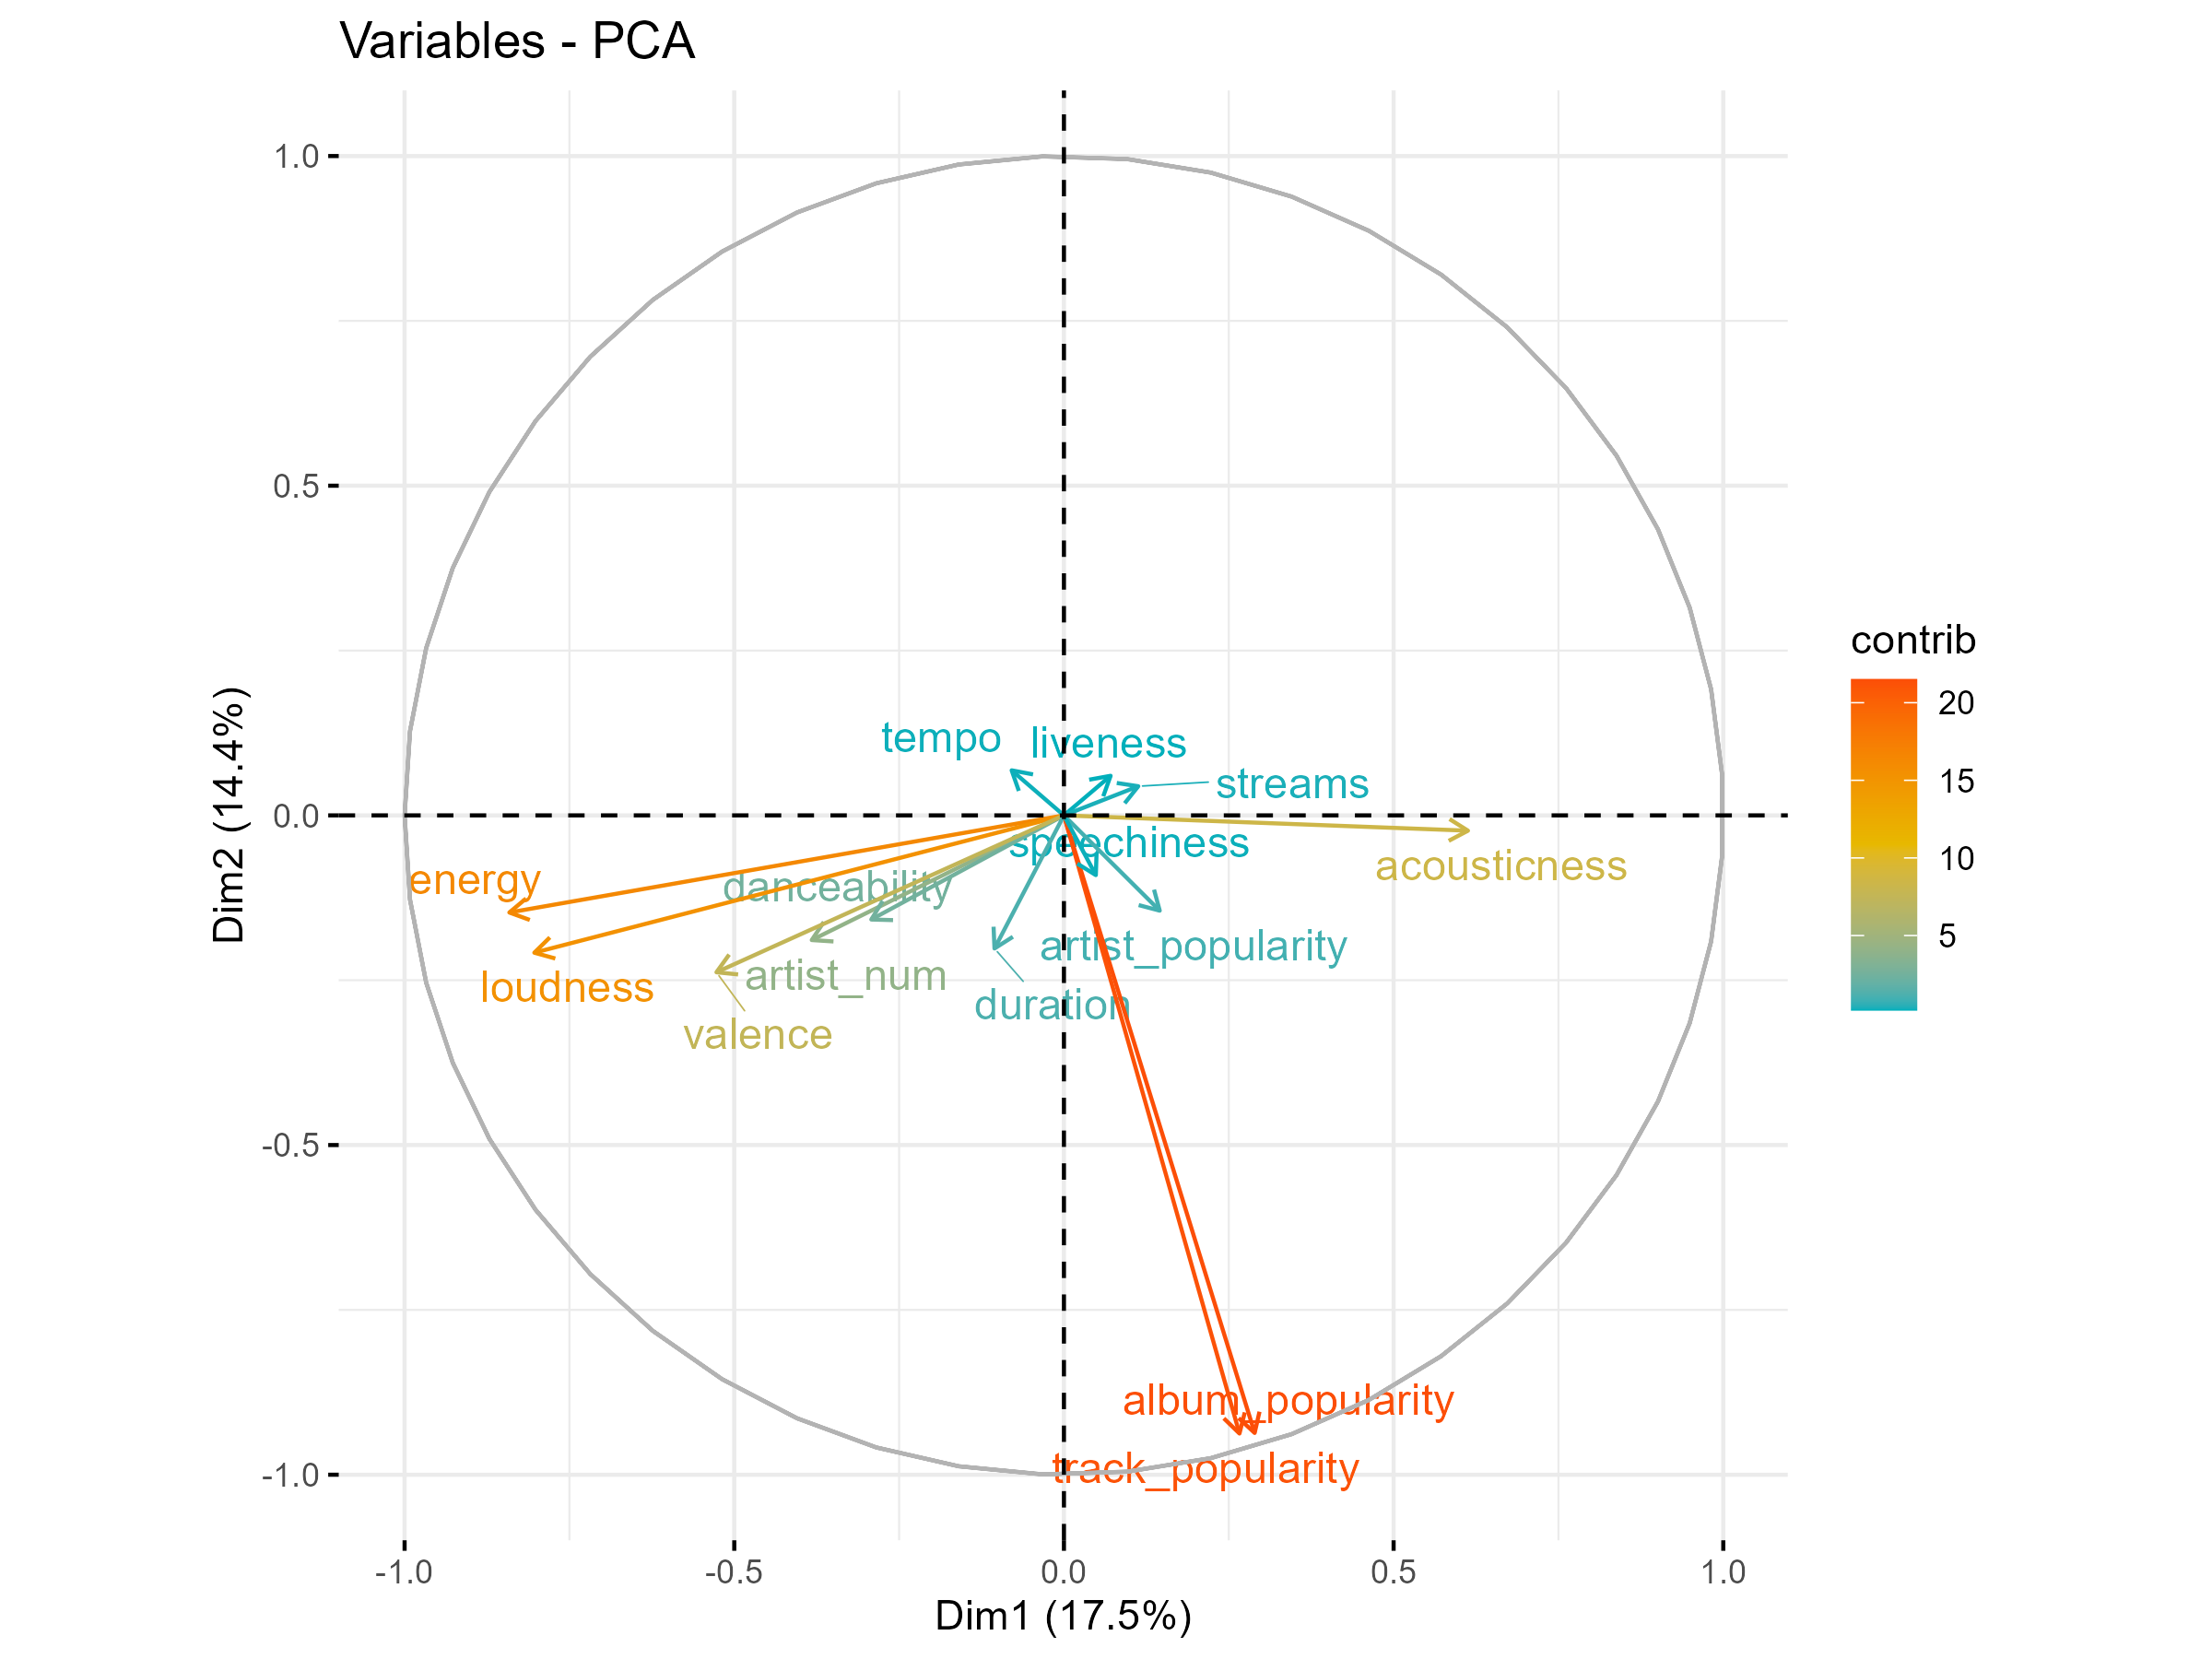
\includegraphics[width=0.8\textwidth]{Images/4_clustering/DBSCAN/dbscanpcacomponents.png}
    \caption{Variables i la seva contribució en cada un dels dos primers components principals.}
    \label{fig:DBSCAN_pca_contrib}
\end{figure}

Abans de realitzar el DBSCAN, el clústering basat en densitat, s’ha creat un petit k-means per tal d’observar la nostra distribució de dades  (figura \ref{fig:KMEANS}). En aquest cas, s’ha usat una k amb valor 5. Cal destacar que a partir d'aquest moment, usarem unes dades normalitzades ja que les distàncies (concretament, els rangs de valors de les variables) poden afectar a aquests clústers.

\begin{figure}[H]
    \centering
    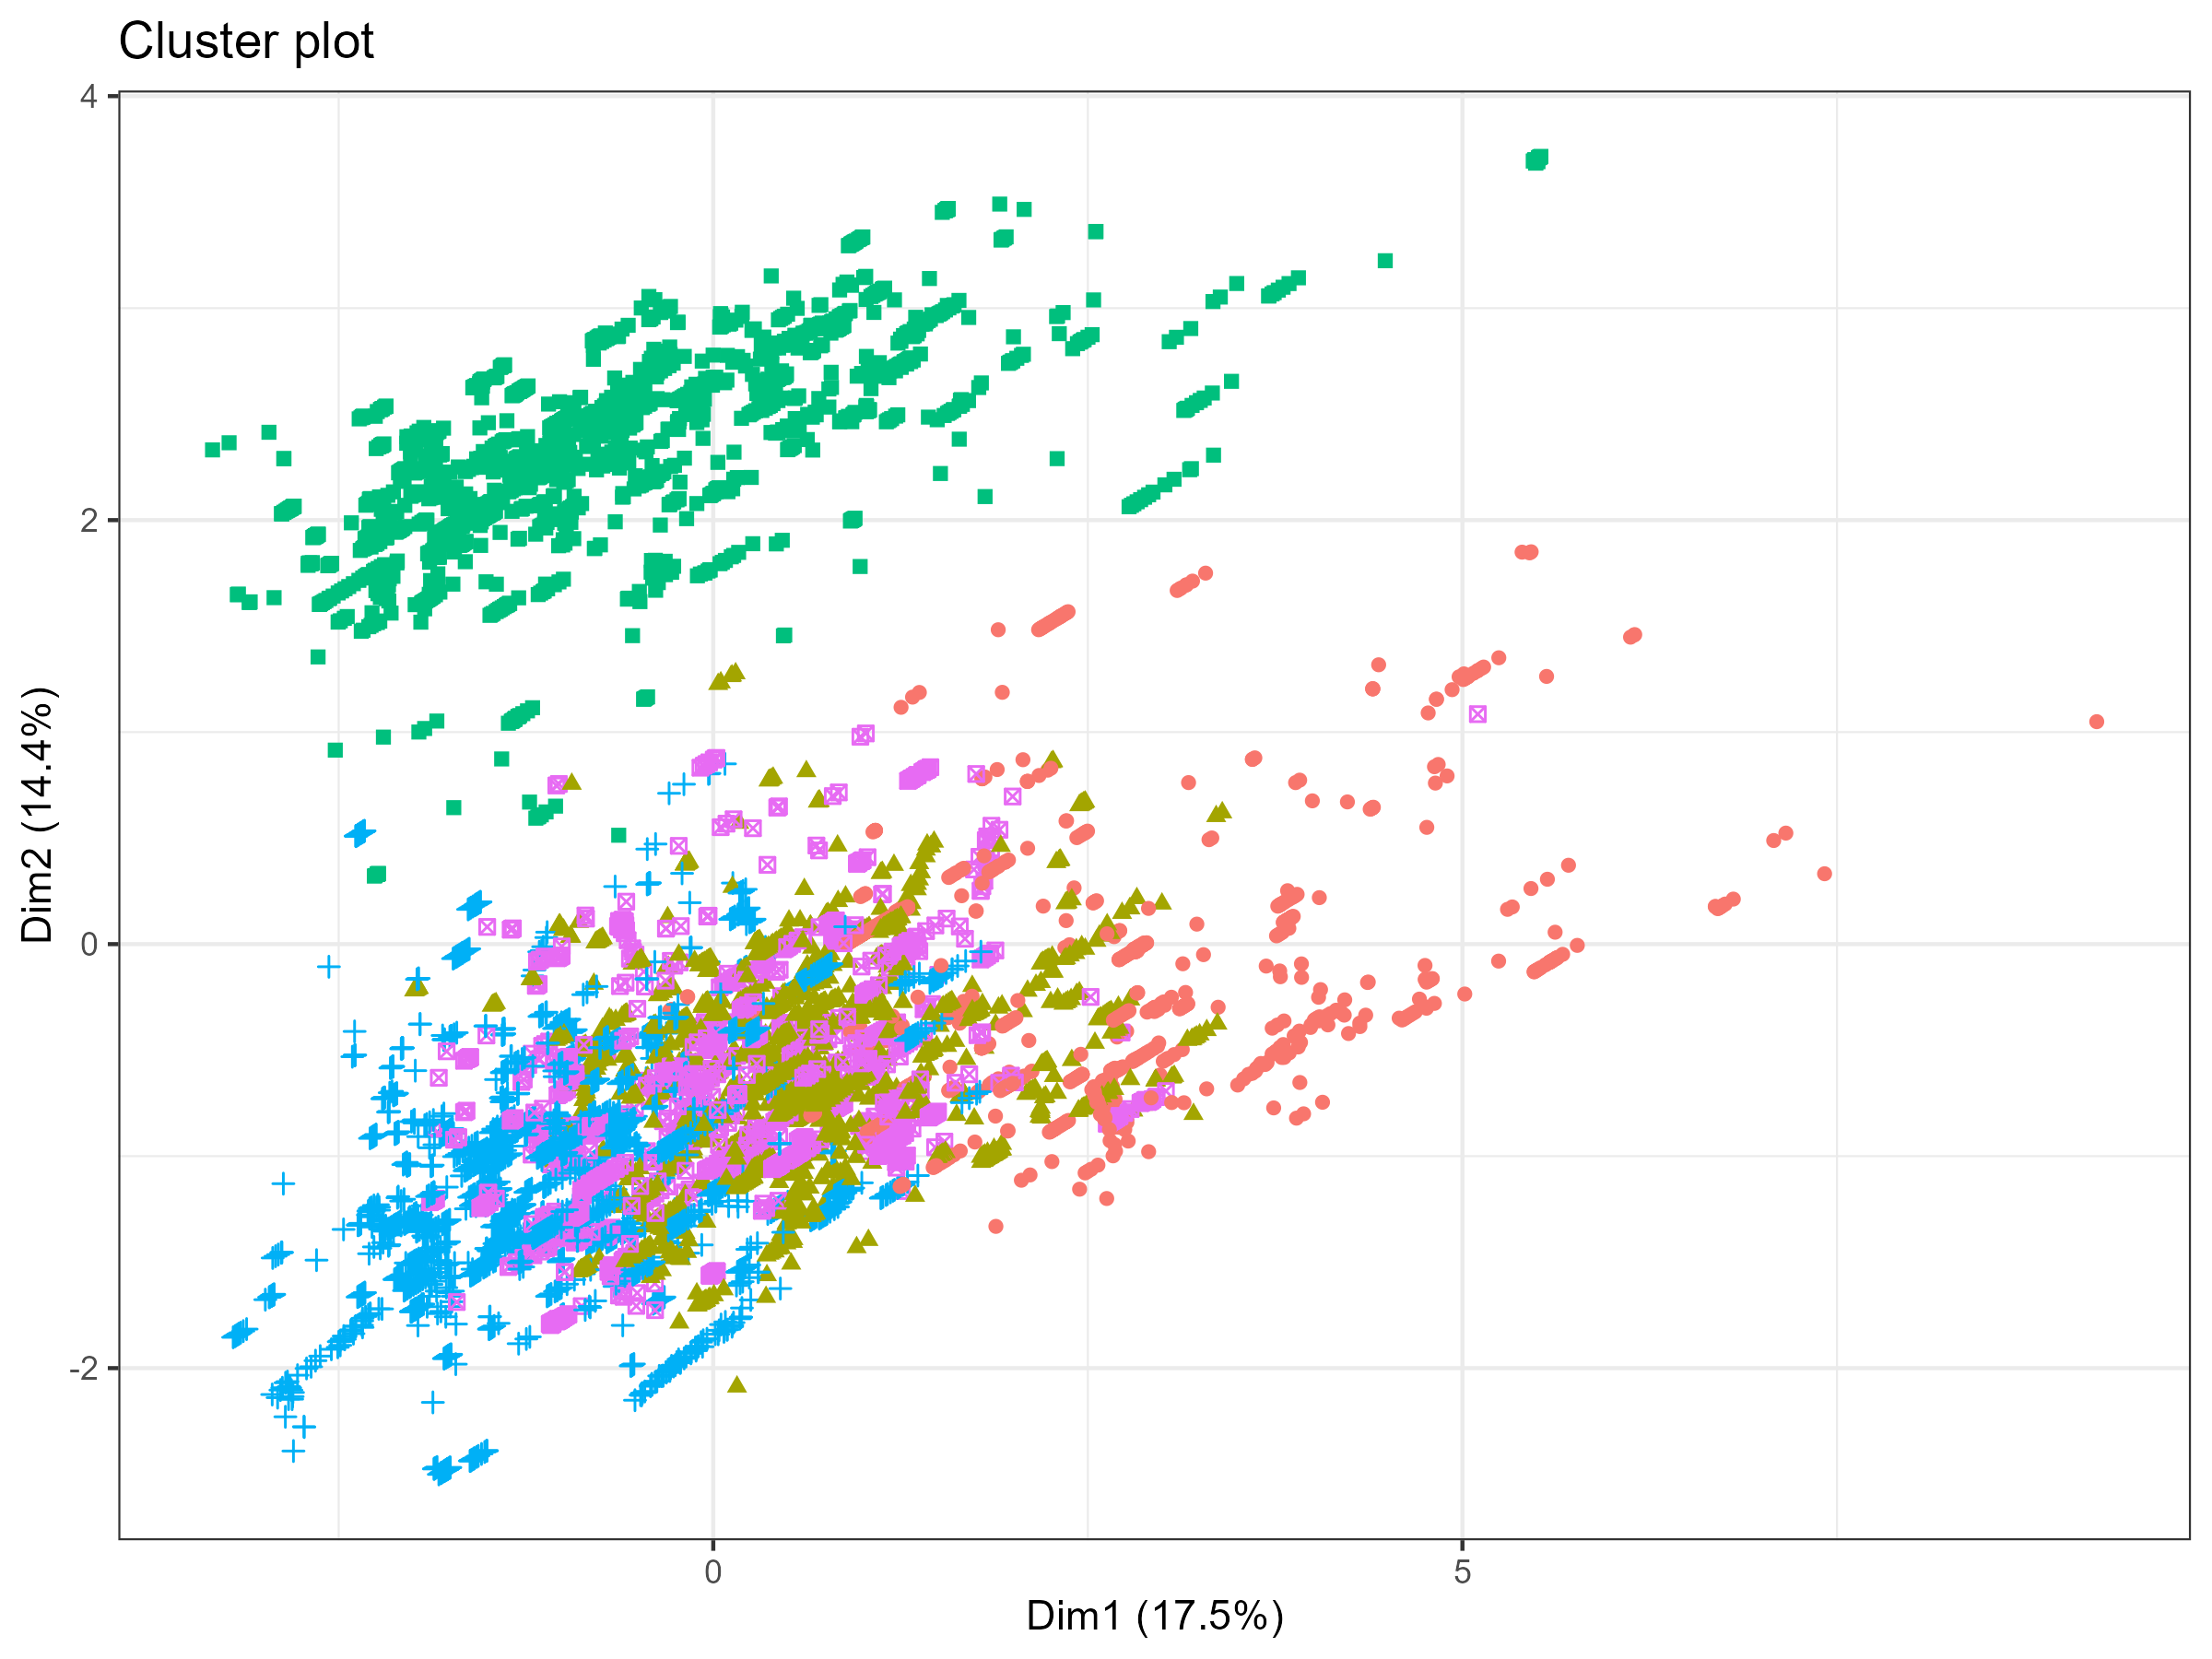
\includegraphics[width=0.8\textwidth]{Images/4_clustering/DBSCAN/kmeans.png}
    \caption{Resultats del clústering usant K-MEANS.}
    \label{fig:KMEANS}
\end{figure}

El grup superior, vist anteriorment, ha estat catalogat pràcticament de manera íntegra en el clúster verd. Pel que fa l’altre, s’ha repartit en funció de la dimensió 1: valors més baixos corresponen al clúster blau, els mitjanament baixos al violeta, els mitjanament alts a un verd més marronós i els alts a un taronja. Els dos clústers amb valors mitjos, el violeta i el marró, han quedat bastant barrejats. En general, però, els clústers creats són bastant bons, i ens serviran de referència per comparar amb els trobats pel DBSCAN.

Observant aquests mateixos clústers en la tercera i quarta dimensió (figura \ref{fig:KMEANS_34}), les dades queden molt més barrejades . Els clústers verds, taronja i marró queden completament inseparables, i els únics que podriem distingir serien el blau, amb valors negatius de la dimensió 3 i el lila amb valors positius. Mirant què representen les dimensions, sembla ser que separa les cançons més aviat llargues i ràpides (lila) contra les més ballables (blau).

\begin{figure}[H]
    \centering
    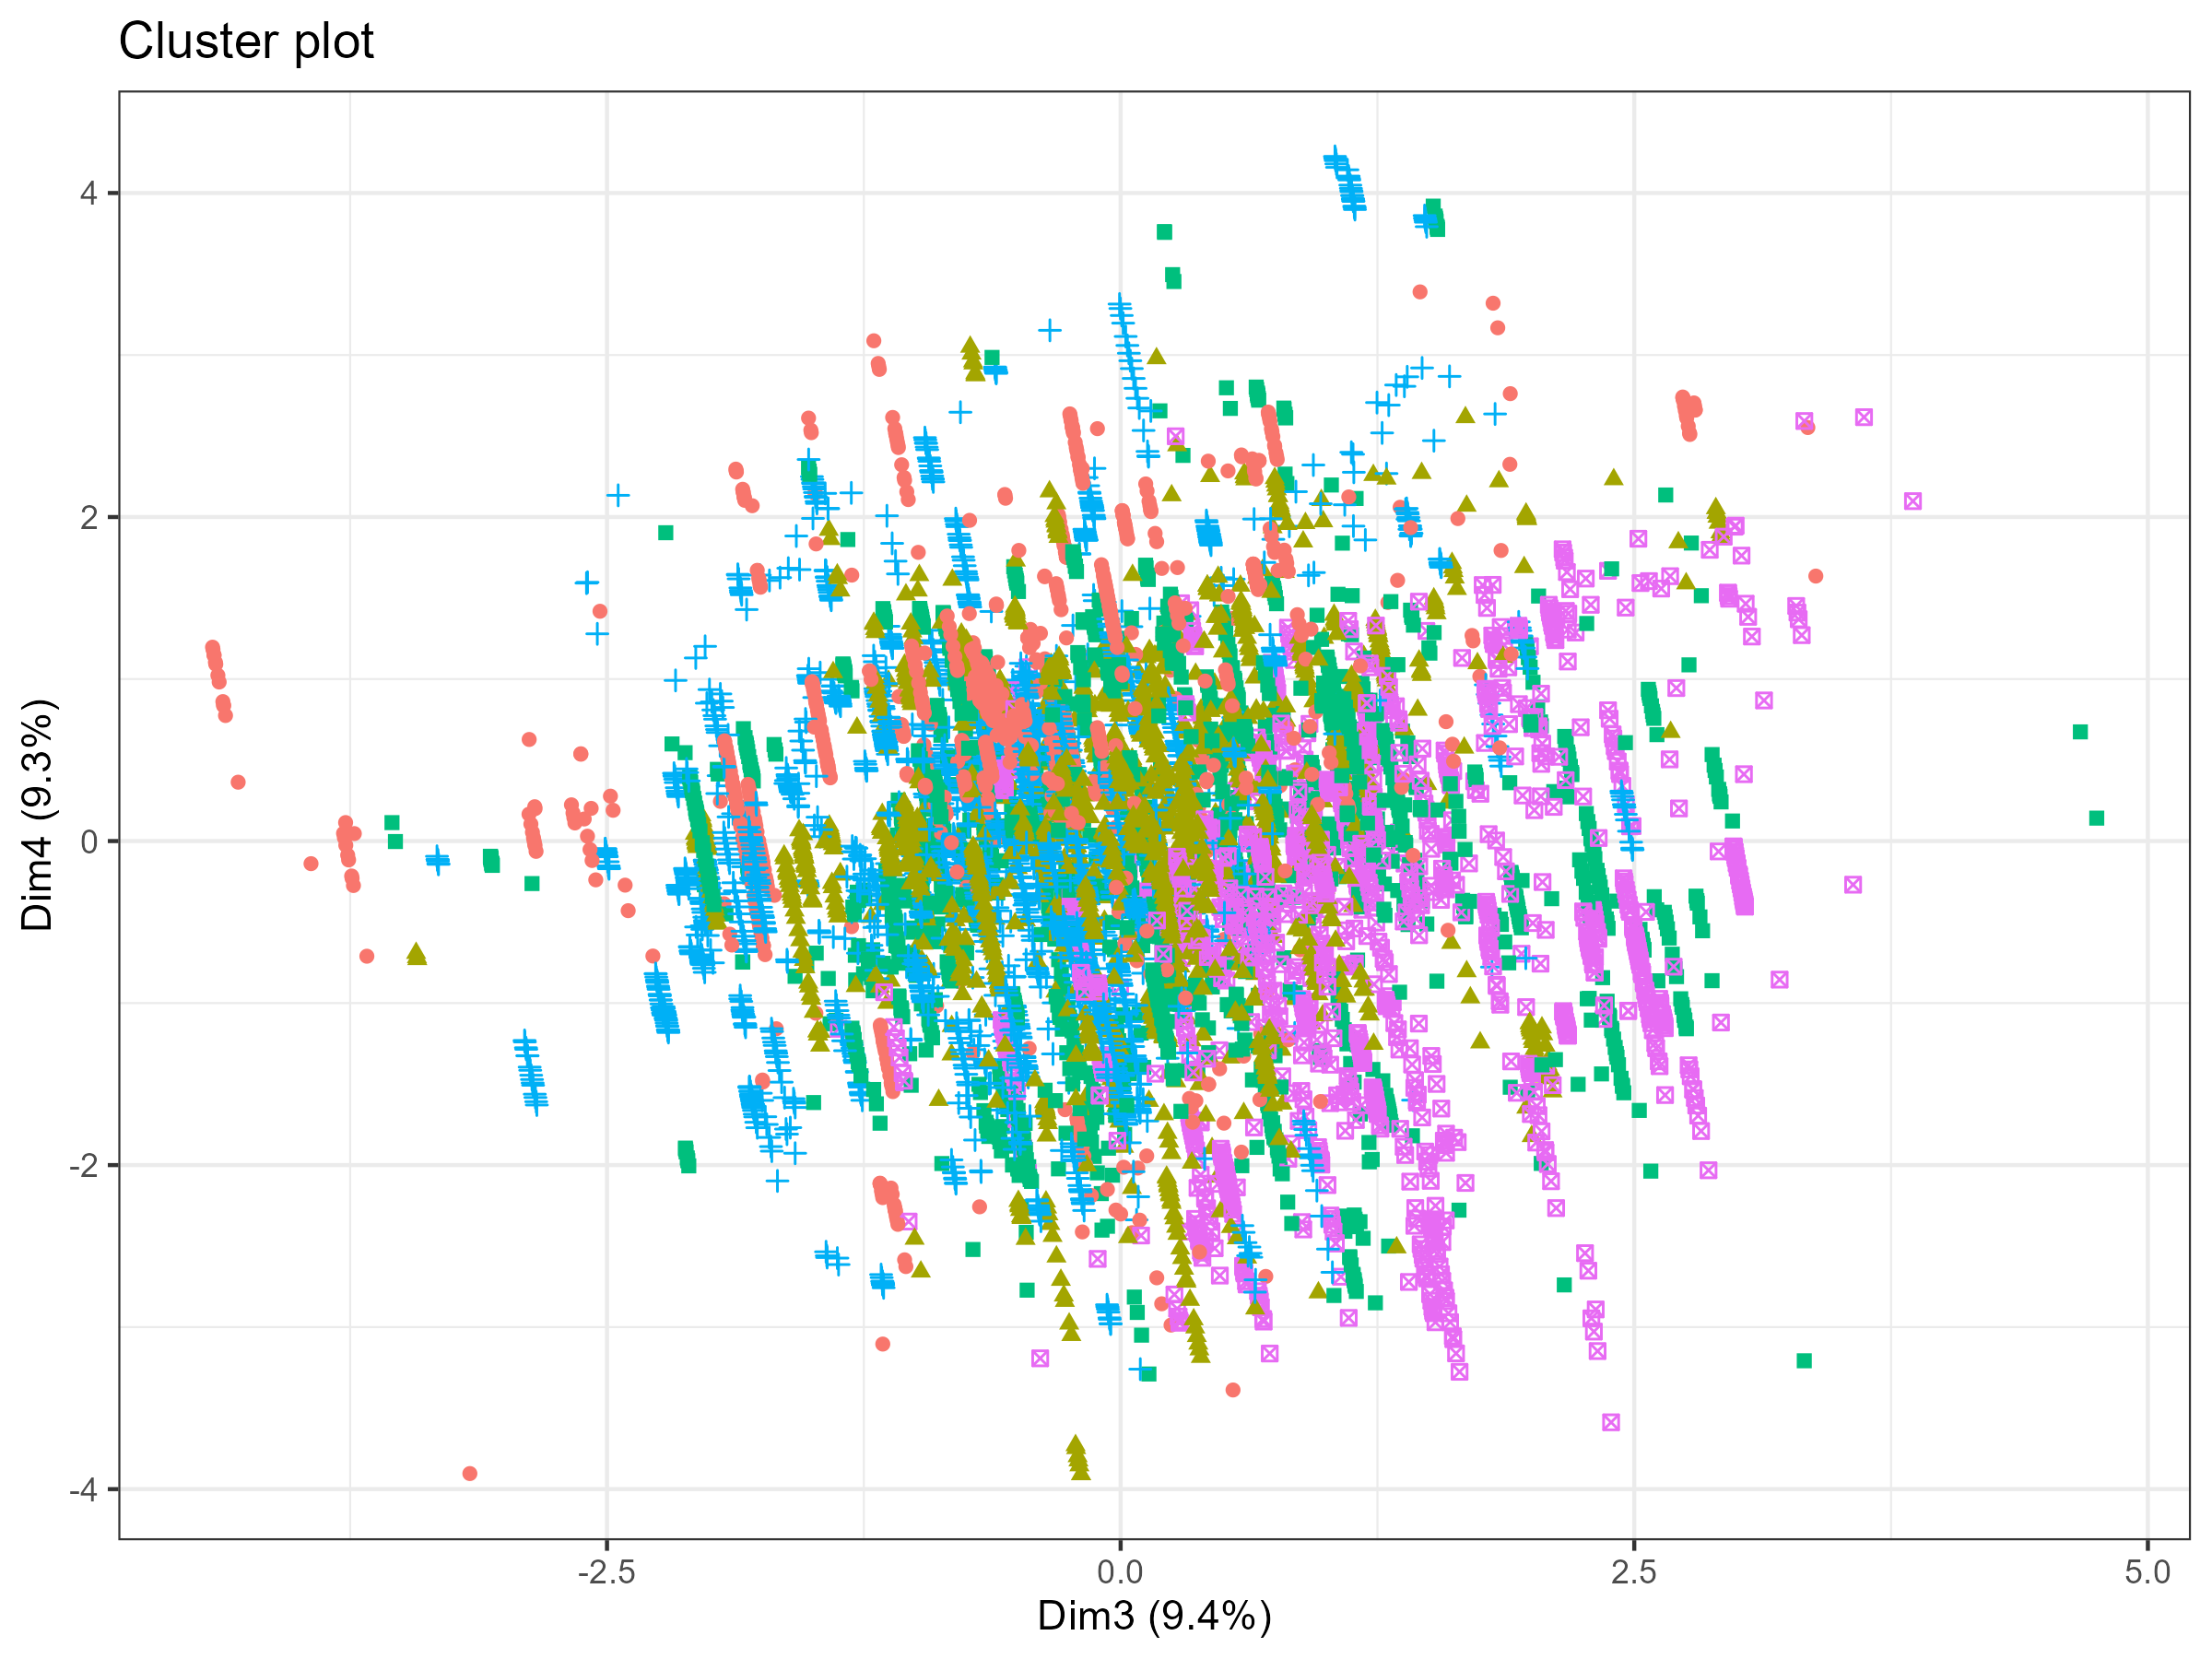
\includegraphics[width=0.8\textwidth]{Images/4_clustering/DBSCAN/kmeans34.png}
    \caption{Resultats del clústering usant K-MEANS visualitzats en components principals 3 i 4}
    \label{fig:KMEANS_34}
\end{figure}

Passant ja al DBSCAN, l’inicial (figura \ref{fig:DBSCAN_inicial}) realitzat amb 0.15 de espsilon i minPts 20 senyalava la gran majoria de punts com outliers, representats com a punts negres transparents. A més, creava molts clústers però molt petits (més de 100 clústers).

\begin{figure}[H]
    \centering
    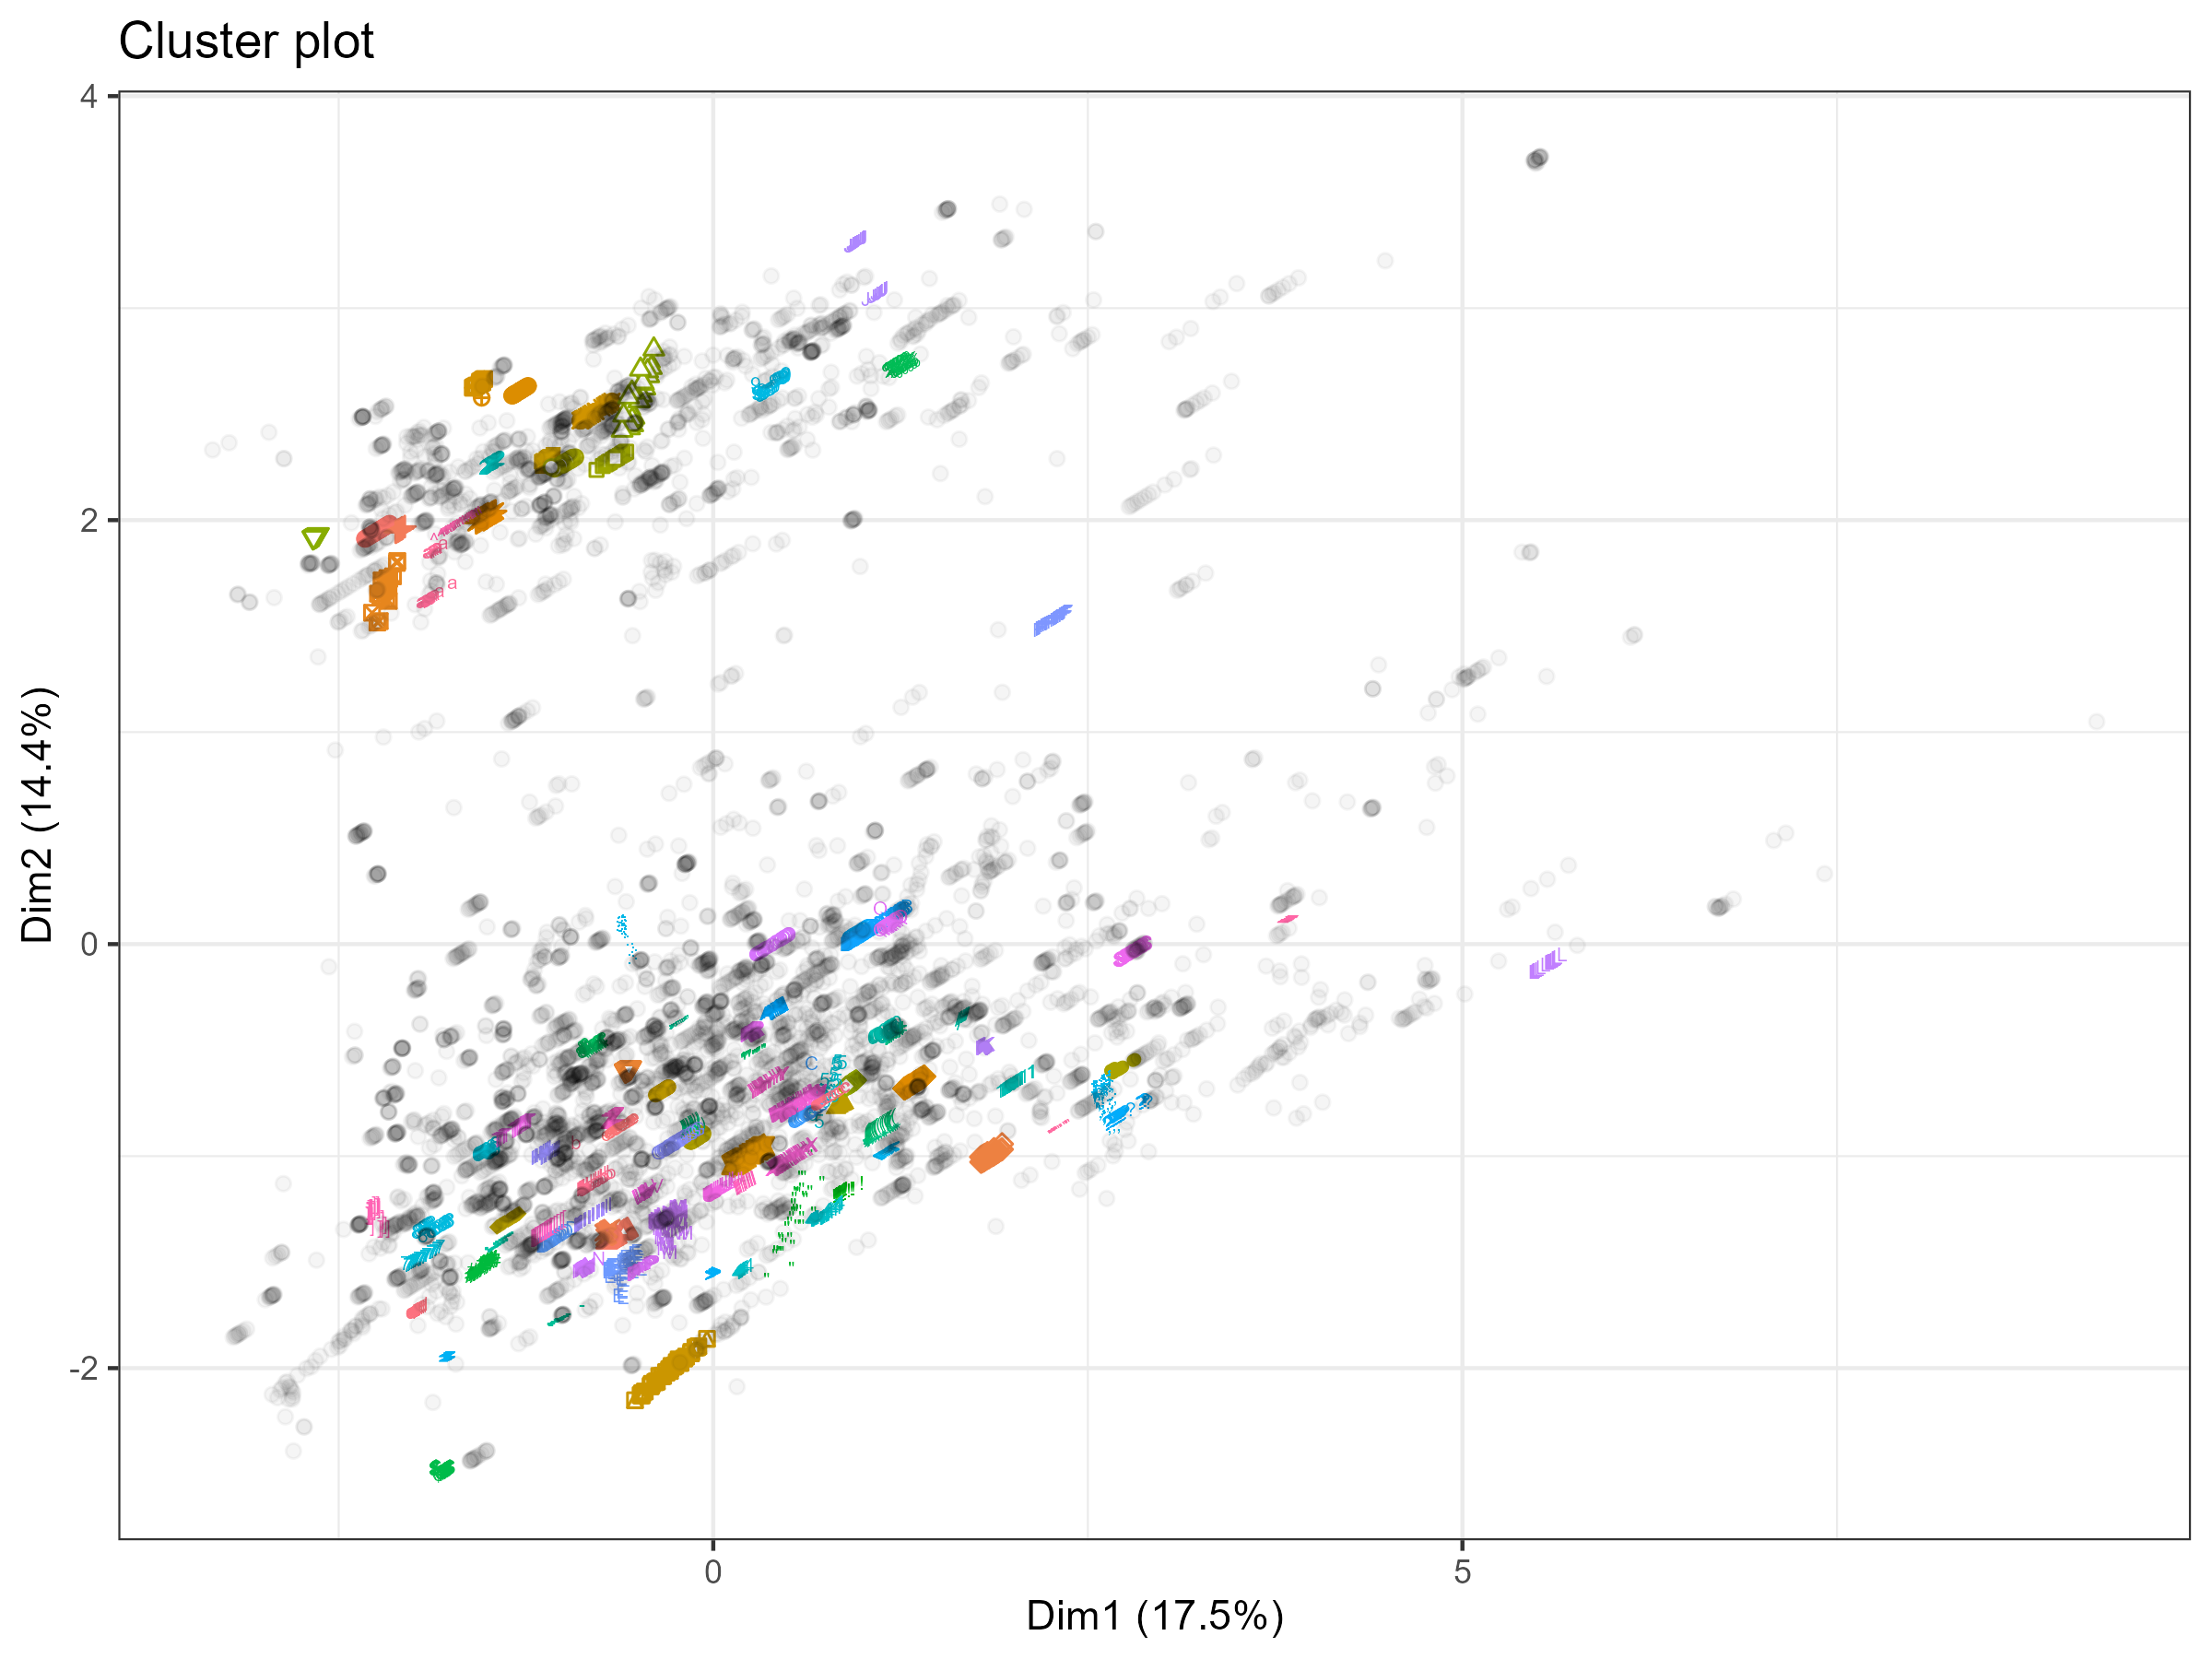
\includegraphics[width=0.8\textwidth]{Images/4_clustering/DBSCAN/baddbscan.png}
    \caption{Resultats del clústering inicial usant DBSCAN (0.15, 20) visualitzats en els dos primers components principals \\
    Des d'aquest punt tots els clústerings seran visualitzats d'aquesta manera.}
    \label{fig:DBSCAN_inicial}
\end{figure}


Per millorar els resultats, calia trobar la millor epsilon i el millor mínim de punts. Pel mínim de punts, es va escollir el 0.25\%, en aquest cas 22 punts. És un valor gran, però cal tenir en compte que la nostra base de dades també és bastant gran, amb 8800 observacions. Per escollir la epsilon, s'han realitzat les distàncies de knn, i s'ha intentat escollir el que tenia canvi de pendent màxim. Aquest retornava una epsilon de 0.72, però analitzant el gràfic s'ha determinat que un millor valor era 0.55. Tornant a realitzar el DBSCAN obteniem la figura  (figura \ref{fig:DBSCAN_auto}):

\begin{figure}[H]
    \centering
    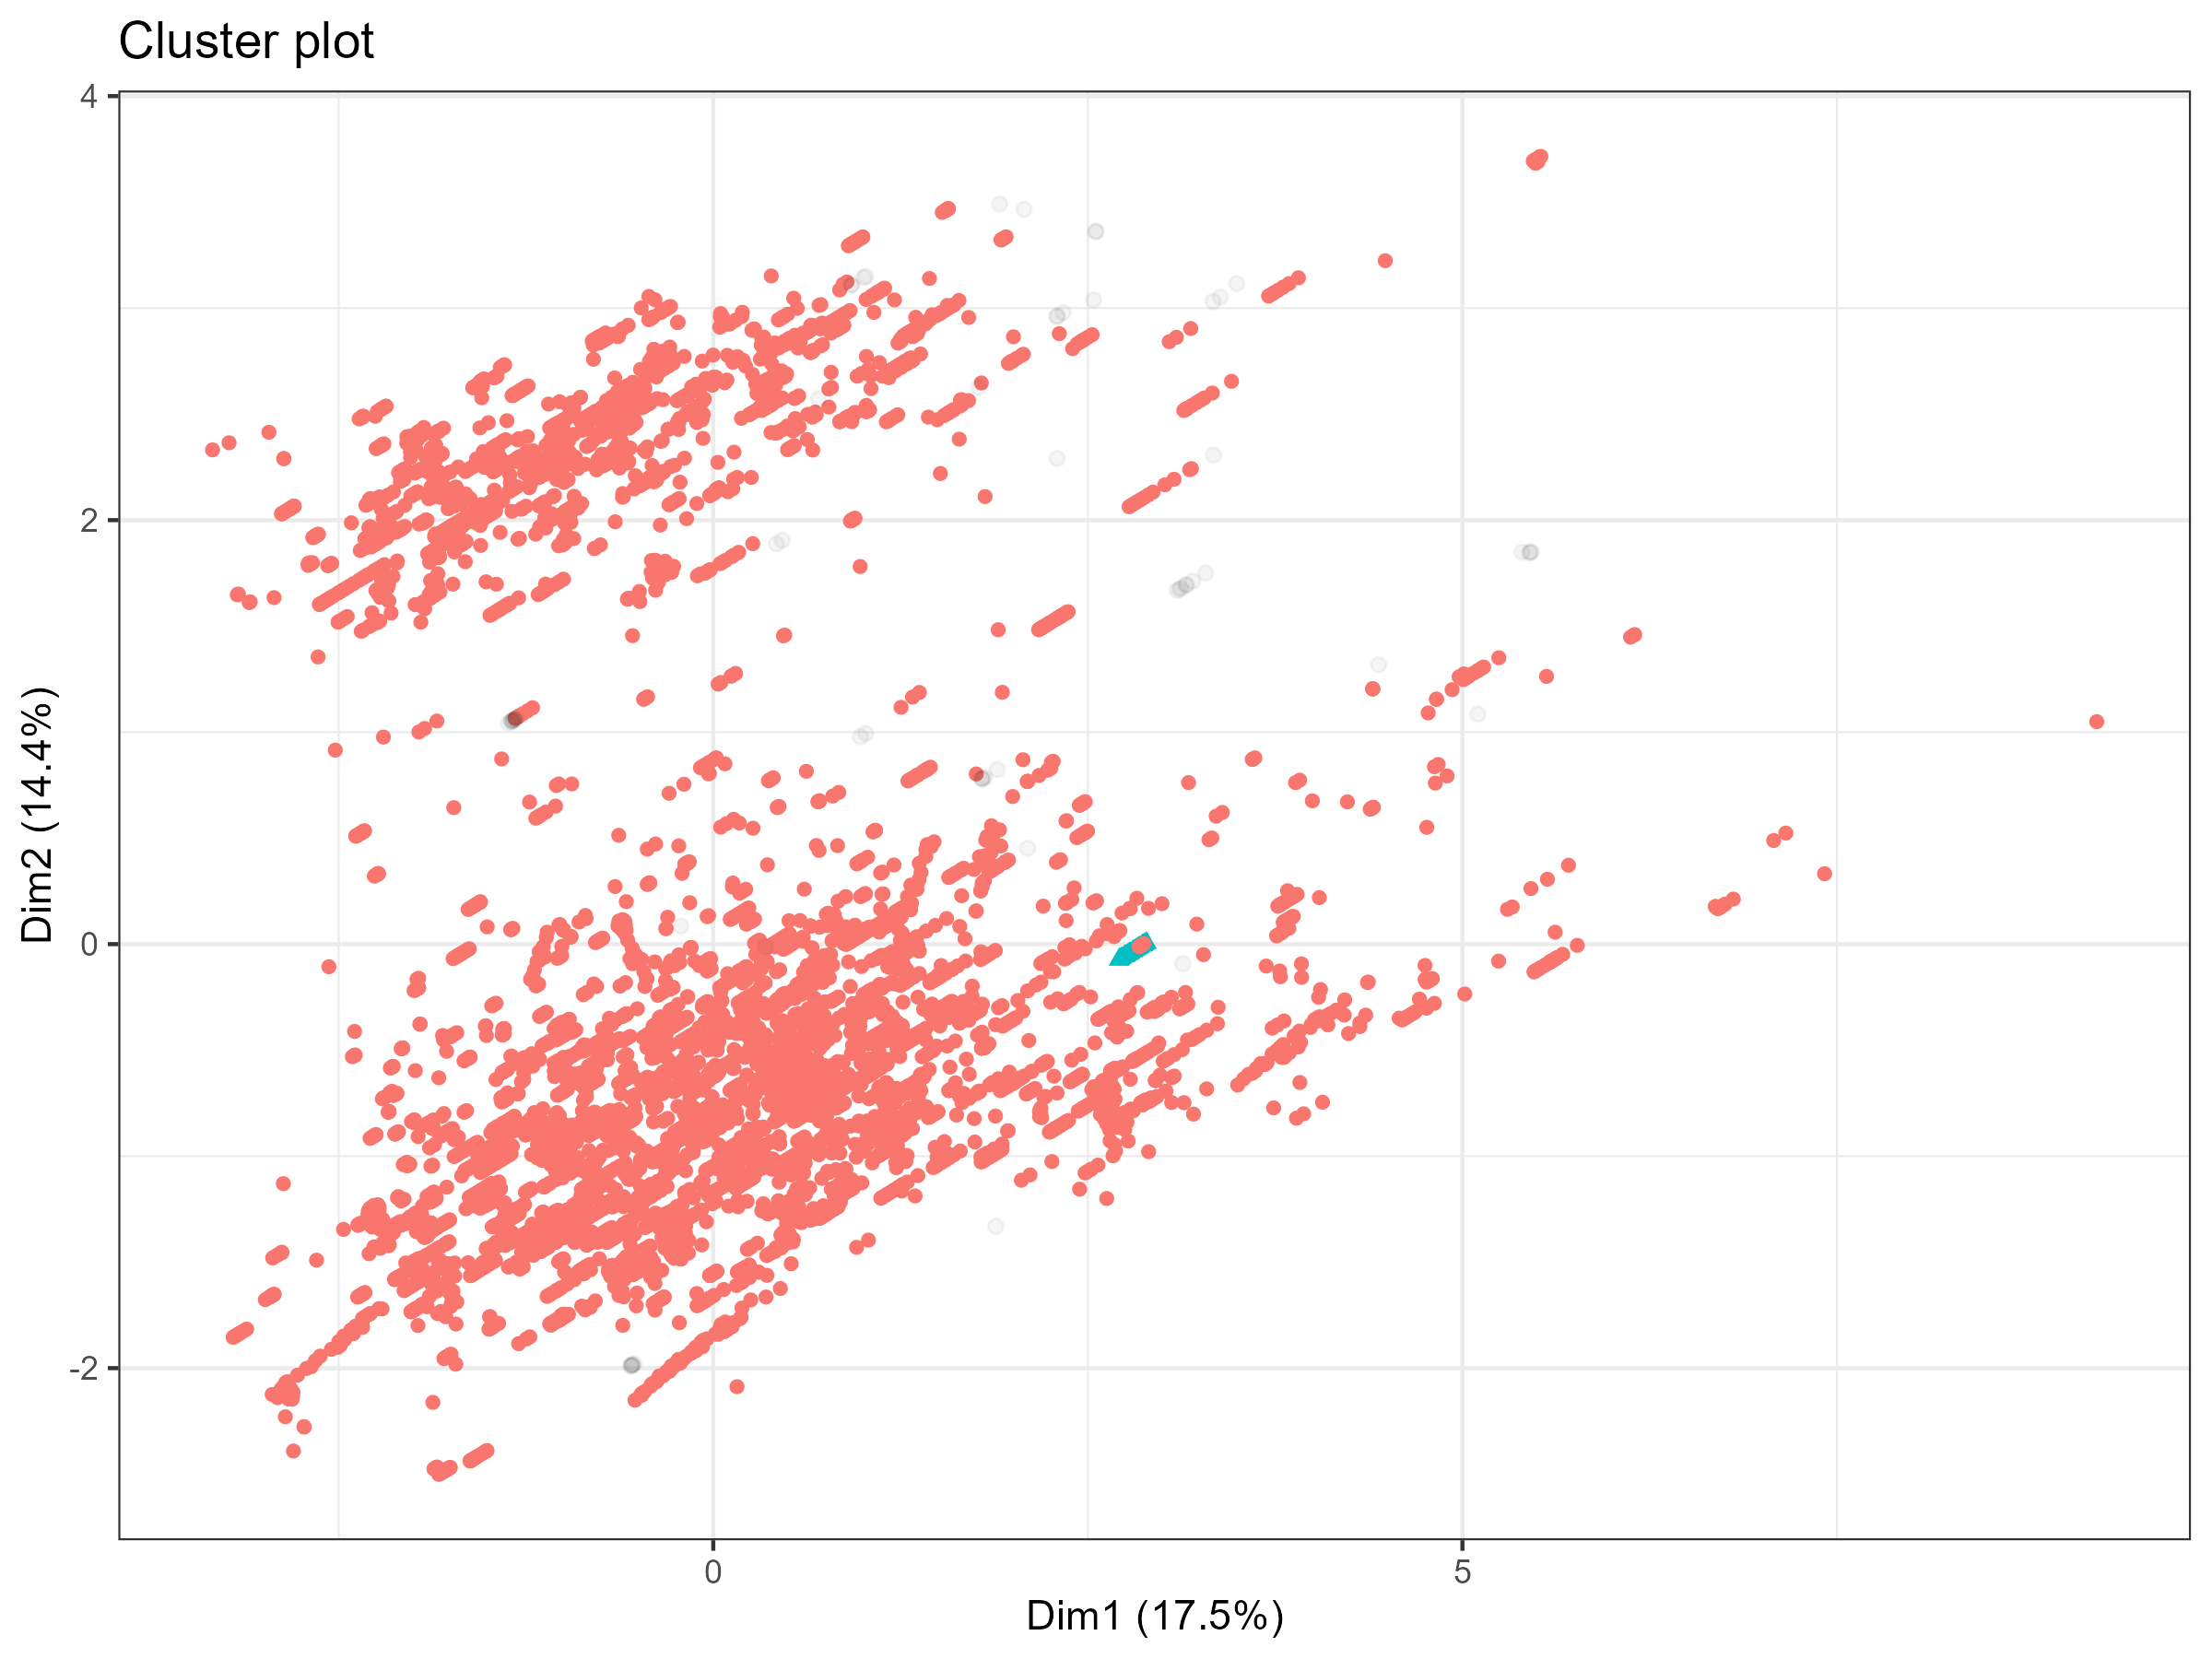
\includegraphics[width=0.8\textwidth]{Images/4_clustering/DBSCAN/dbscanauto.png}
    \caption{Resultats del clústering usant DBSCAN, epsilon knn (0.55, 22)}
    \label{fig:DBSCAN_auto}
\end{figure}

Es pot veure com aquests valors no han servit gens per millorar els resultats: ara, enlloc d'haver-hi molts clústers petits, n'hi ha un de molt gran. En teoria n'hi ha dos més, però son tan petits que són pràcticament imperceptibles.

Buscant de forma artificial uns valors de èpsilon i de mínim de punts, el resultat del DBSCAN ha sigut millor (figura \ref{fig:DBSCAN_manual}), tot i que no ha variat gaire respecte al k means: hem trobat els dos grans grups esmentats anteriorment. Per fer-ho, s'ha usat una epsilon de 0.4 i un mínim de punts de 70 (molt elevat). Amb valors més petits de mínim de punts, apareixien altre cop els clústers molt petits, que no aporten gaire res. Jugant amb la epsilon (per exemple, 0.35) es van obtenir alguns clústers dins del clúster gran de baix: un amb els valors més baixos de la dimensió 2, un altre amb els valors més alts de la dimensió 1 i un altre amb valors alts de les dues dimensions (figura \ref{fig:DBSCAN_manual2}). Tot i això, aquests clústers eren bastant petits.

\begin{figure}[H]
    \centering
    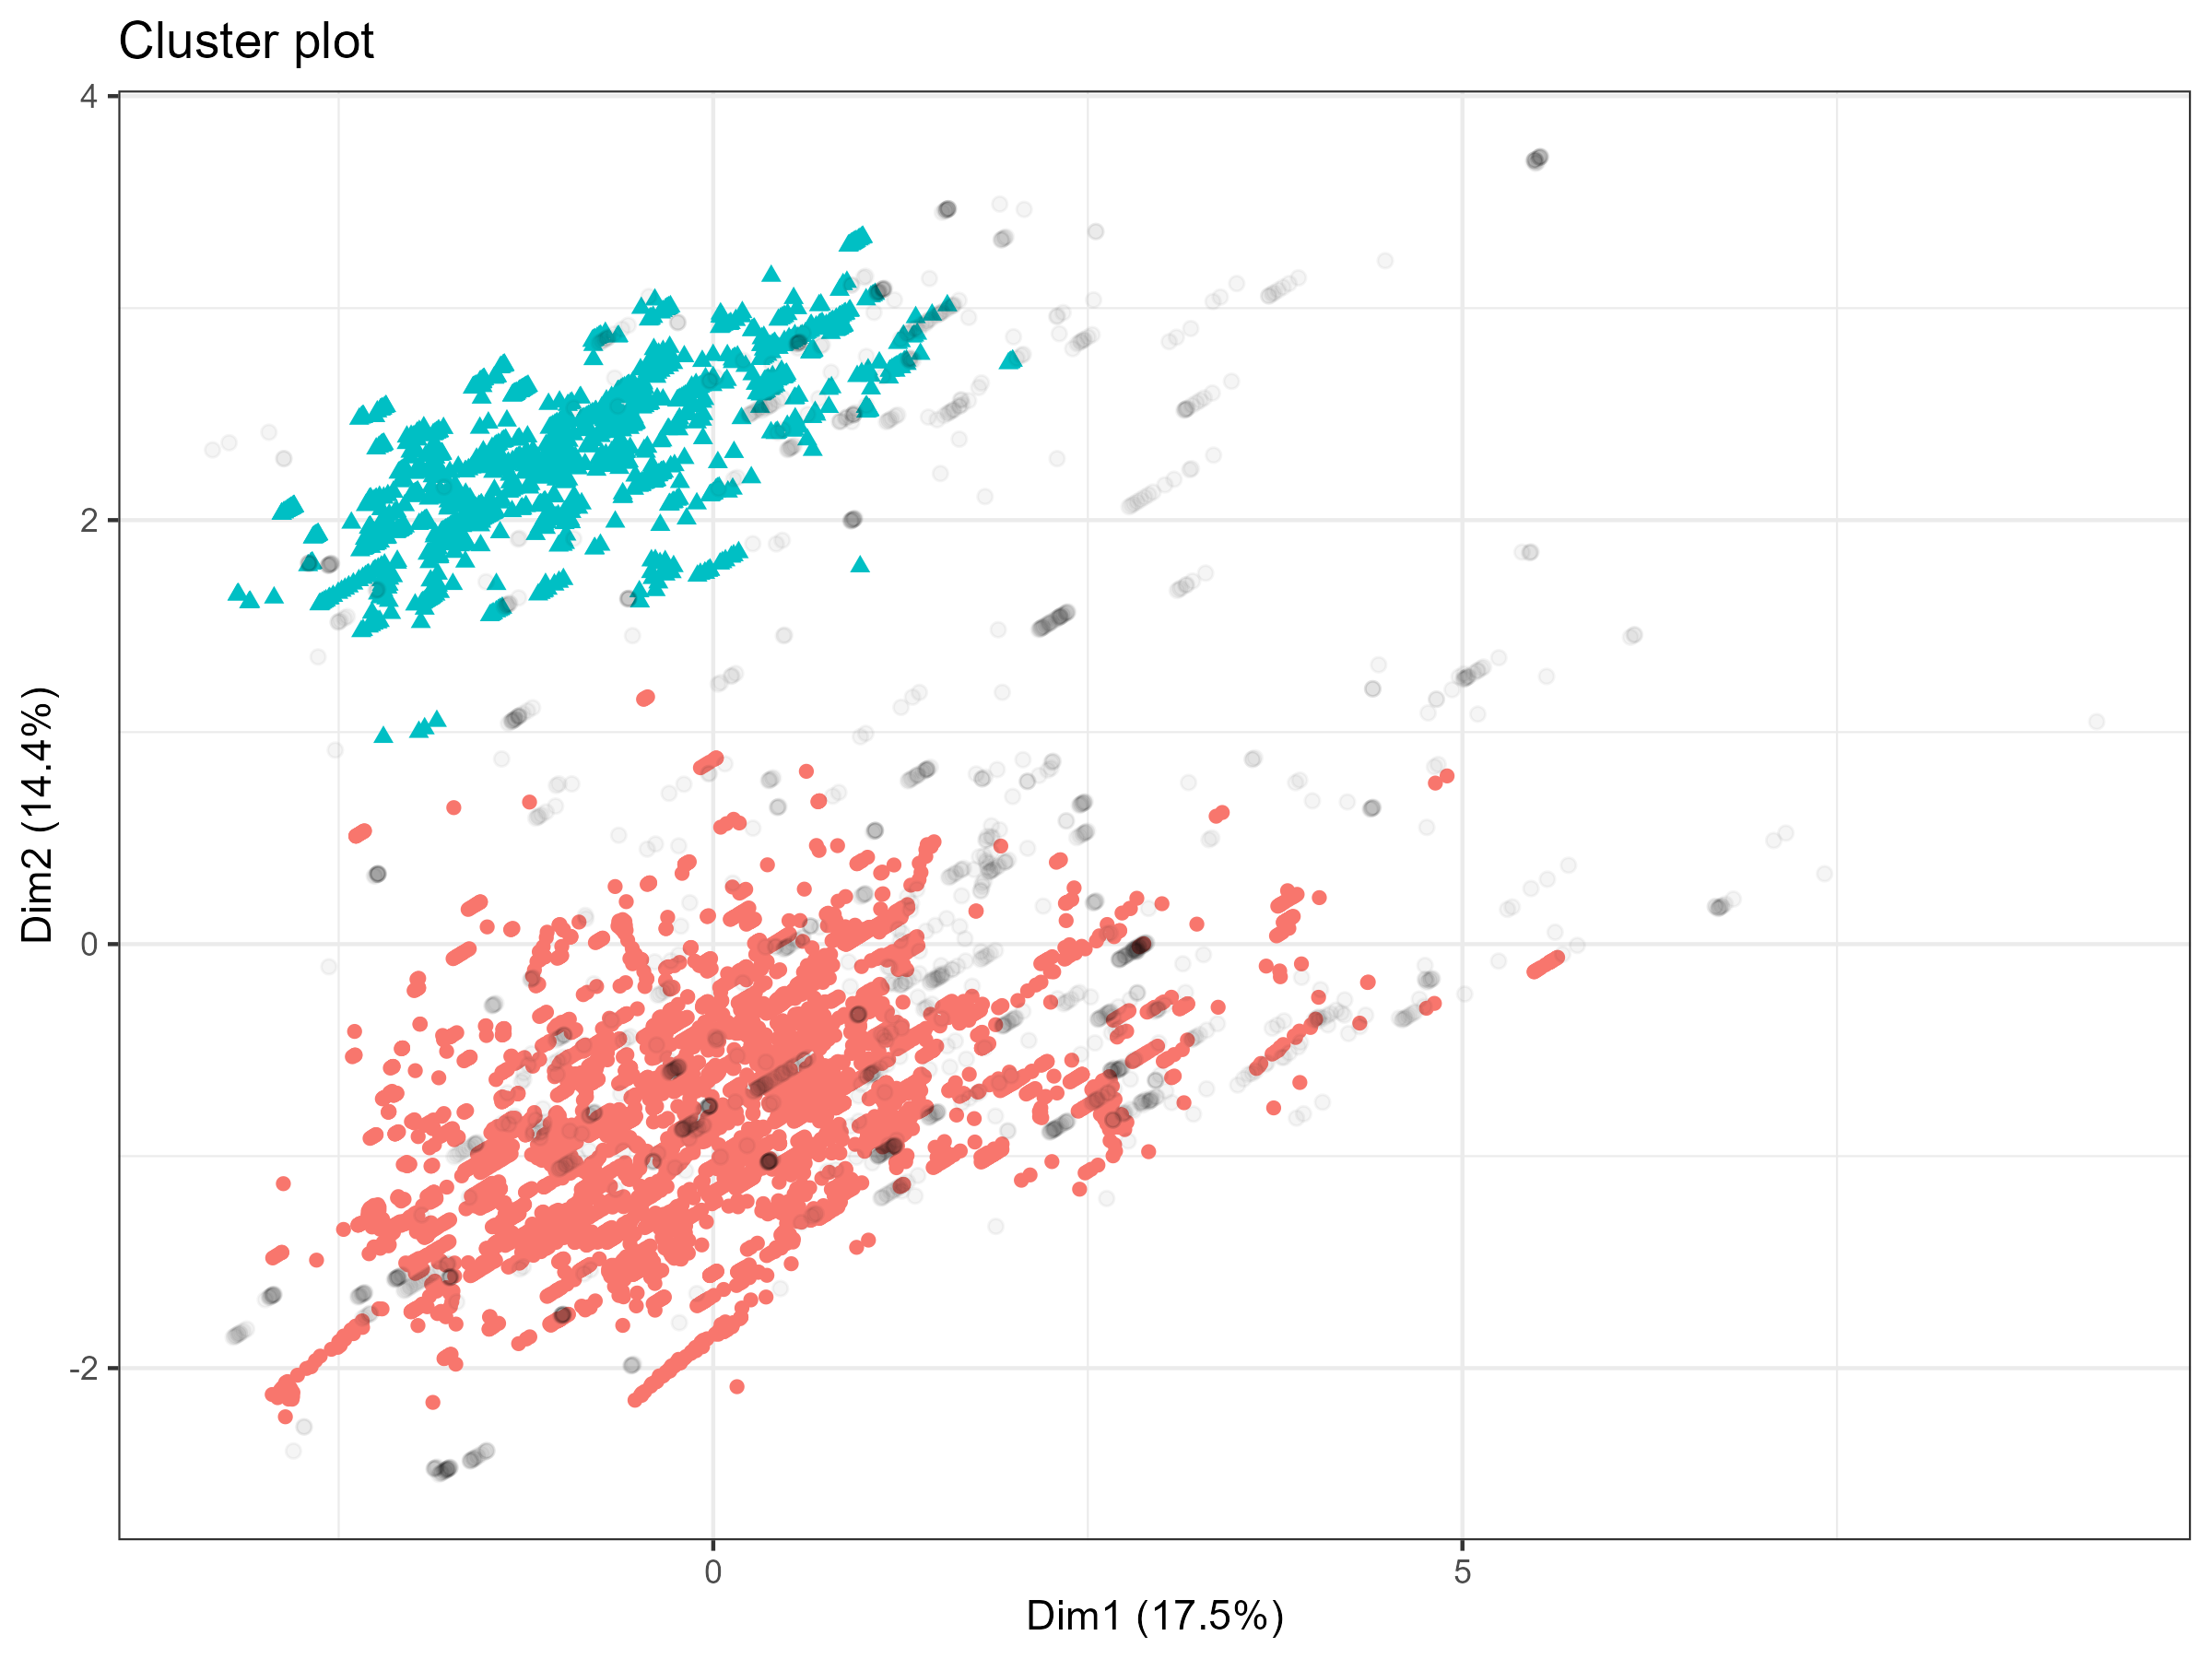
\includegraphics[width=0.8\textwidth]{Images/4_clustering/DBSCAN/dbscanforca.png}
    \caption{Resultats del clústering usant DBSCAN, epsilon manual (0.4, 70)}
    \label{fig:DBSCAN_manual}
\end{figure}

\begin{figure}[H]
    \centering
    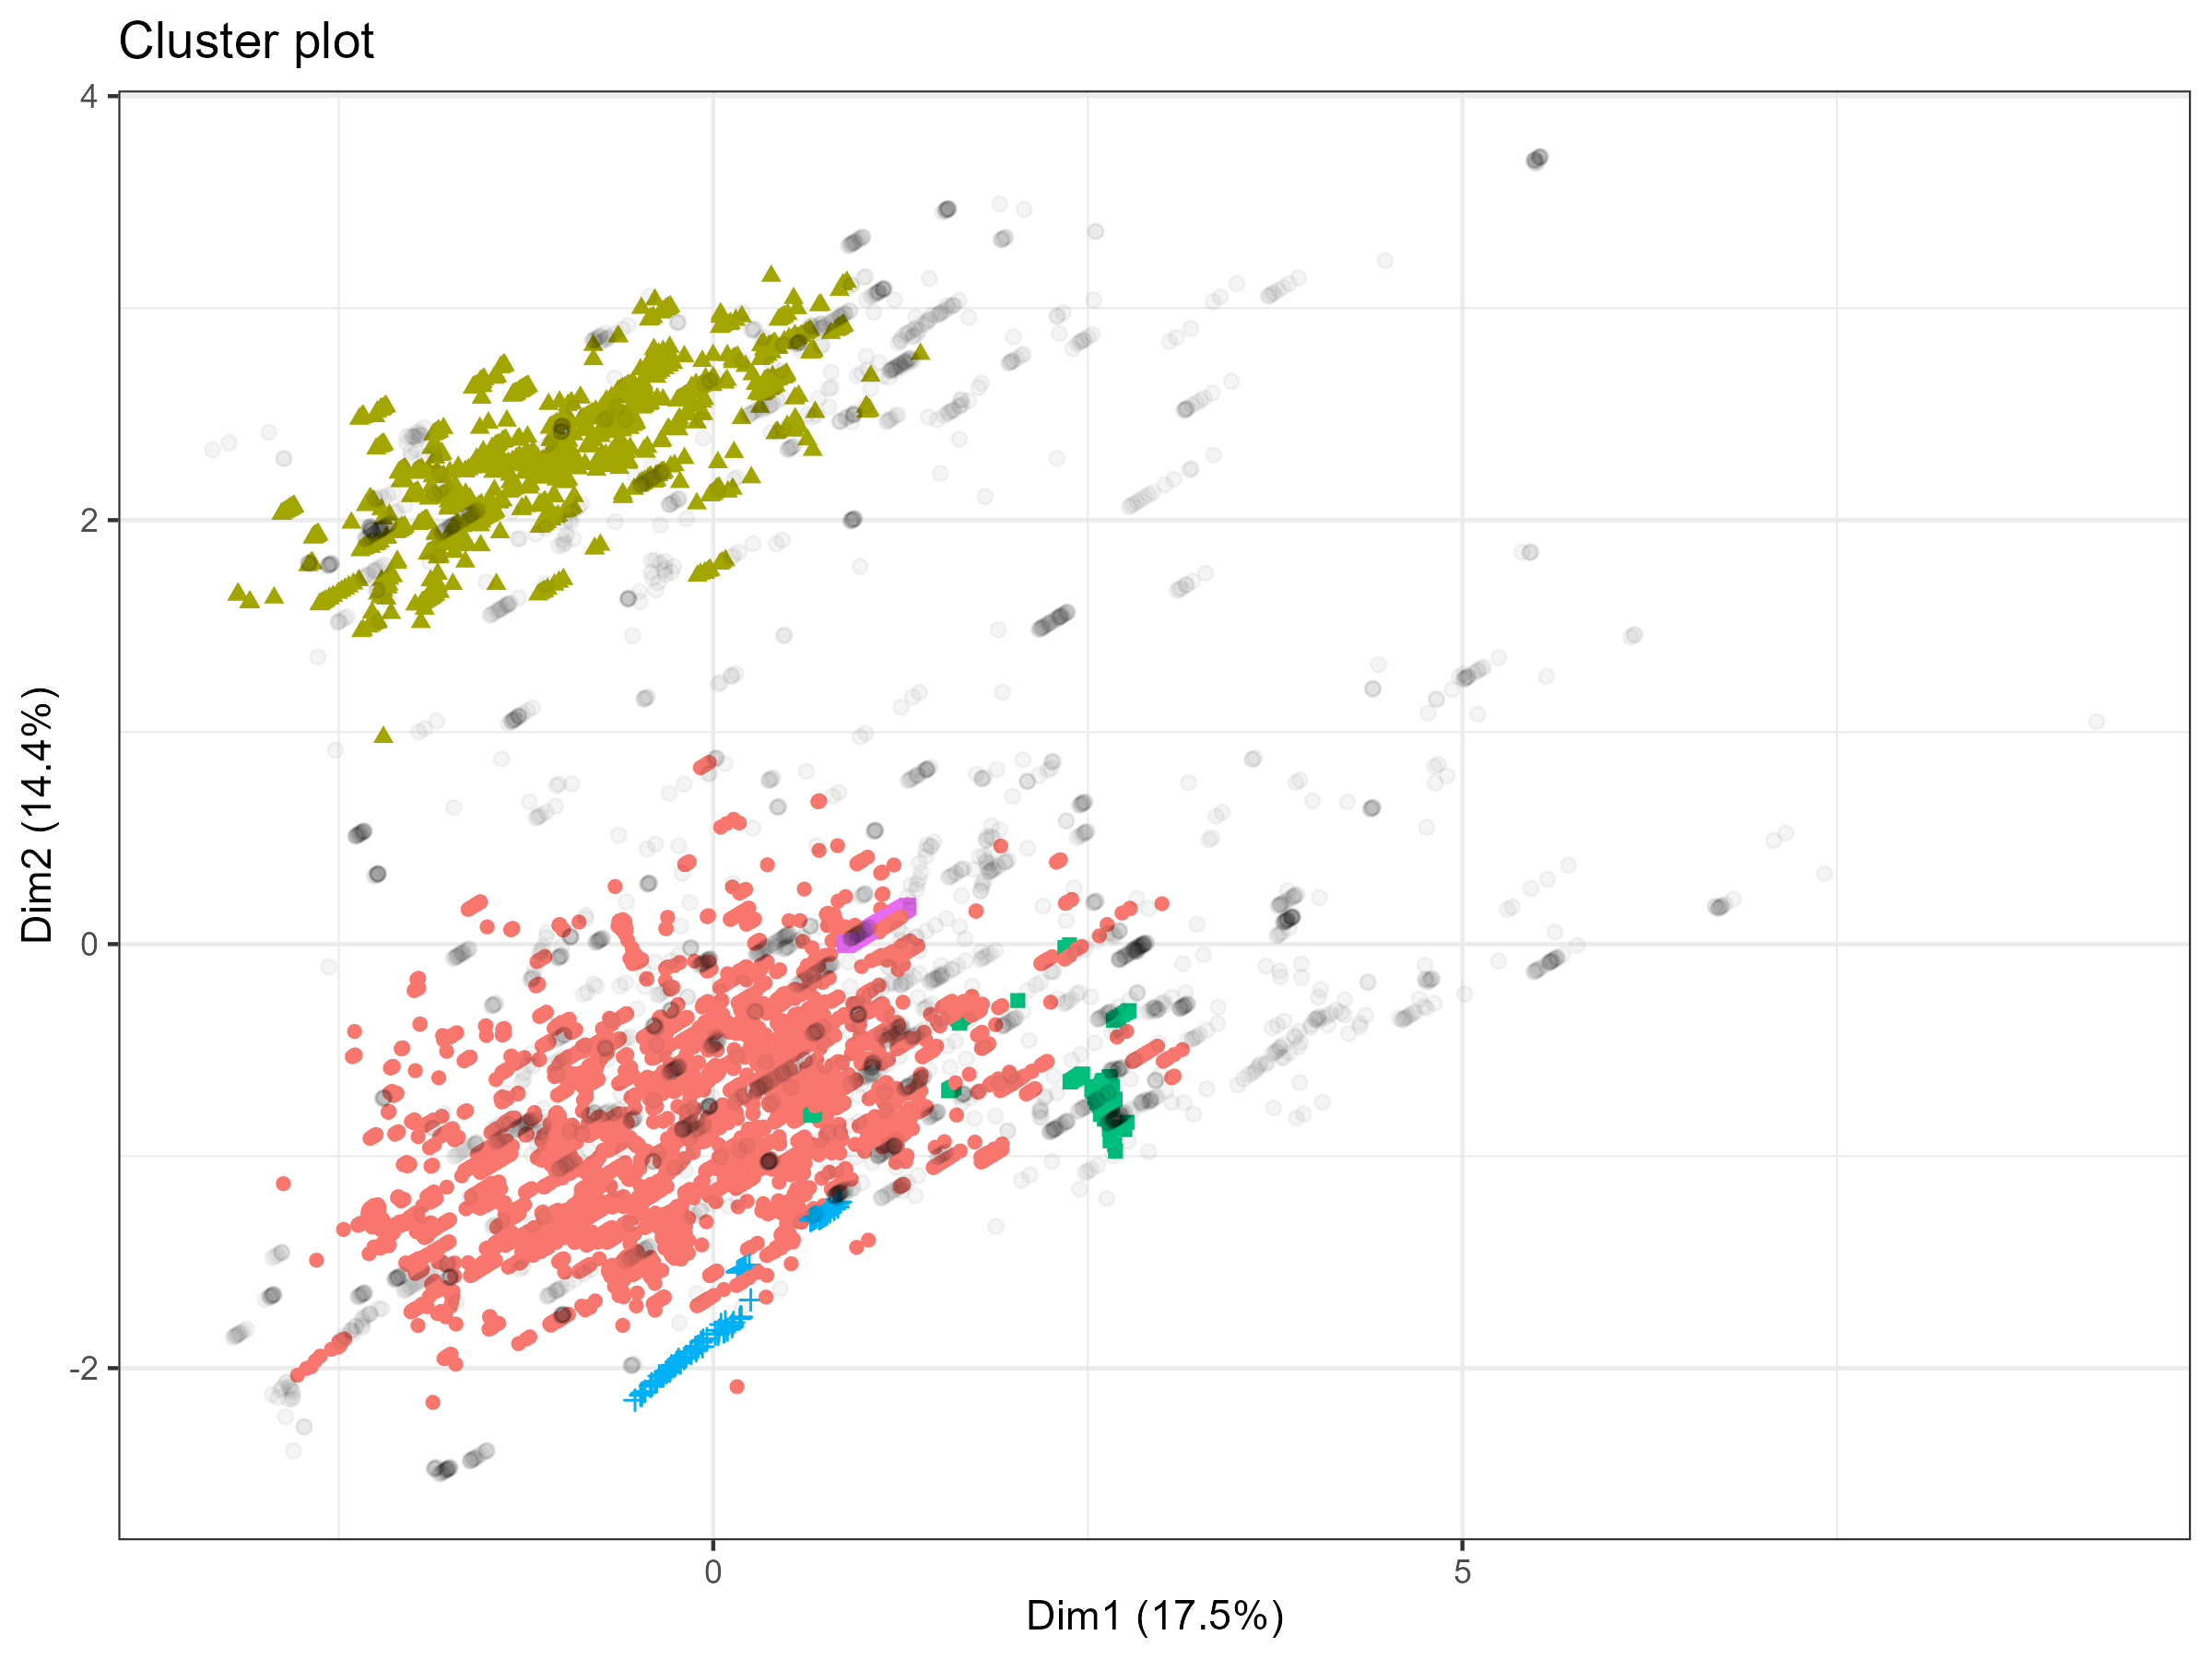
\includegraphics[width=0.8\textwidth]{Images/4_clustering/DBSCAN/dbscanforcaalt.png}
    \caption{Resultats del clústering usant DBSCAN, epsilon manual v2 (0.35, 70)}
    \label{fig:DBSCAN_manual2}
\end{figure}

En aquest apartat, el clústering escollit després de valorar totes les opcions ha sigut el DBSCAN usant epsilon 0.47 i minPts 70. Amb aquest obtenim les dues classes que s'han comentat, i 508 outliers.

A més del DBSCAN, es plantejava usar un algorisme derivat d’aquest, però que usa una tècnica diferent: OPTICS (\cite{ankerst_1999_optics}). Aquest analitza on “pot anar” cada punt, assignant-li una \textit{reachability}. En la base de dades, el reachability plot, usant els paràmetres epsilon 0.55 i minPts 22 es poden observar a la figura \ref{fig:OPTICS_inicial}.

\begin{figure}[H]
    \centering
    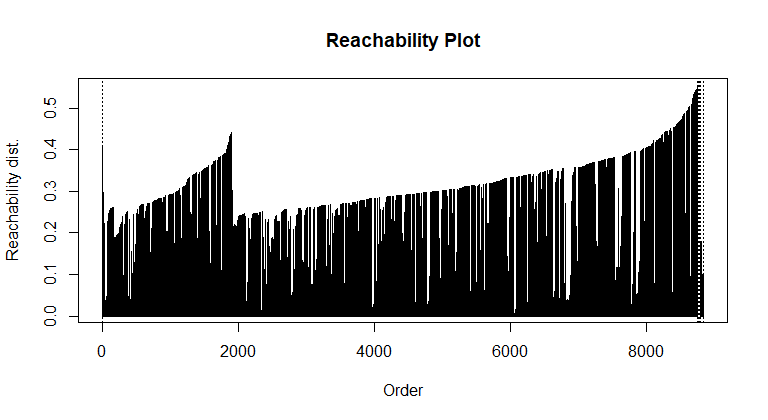
\includegraphics[width=0.8\textwidth]{Images/4_clustering/optics/reachability1.png}
    \caption{Reachability de OPTICS inicial (0.55, 22)}
    \label{fig:OPTICS_inicial}
\end{figure}

Per tal d'escollir un altre epsilon i minPts que anés millor, s'ha provat utilitzant un Grid Search tots els epsilon entre 0.1 i 1 de 0.05 en 0.05 i tots els minPts entre 10 i 70 de 10 en 10. Després d'aquesta cera, els millors valors escollits han estat 0.9 i 10 punts. El Reachability plot queda, tallant a 0.4, tal que (figura \ref{fig:OPTICS_grid}):

\begin{figure}[H]
    \centering
    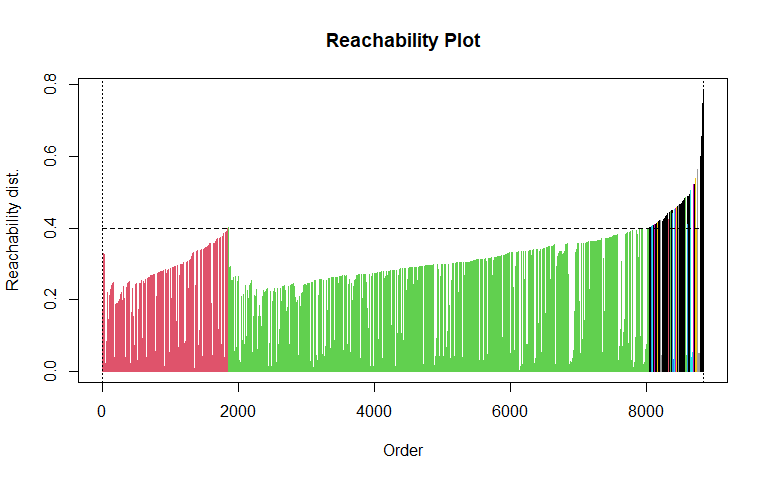
\includegraphics[width=0.8\textwidth]{Images/4_clustering/optics/reachabilitygrid.png}
    \caption{Reachability de OPTICS usant grid search (0.9, 10)}
    \label{fig:OPTICS_grid}
\end{figure}

D'aquí, podem extreure un clústering que es pot visualitzar igual que feiem amb el DBSCAN (figura \ref{fig:OPTICS_grid_res}).

\begin{figure}[H]
    \centering
    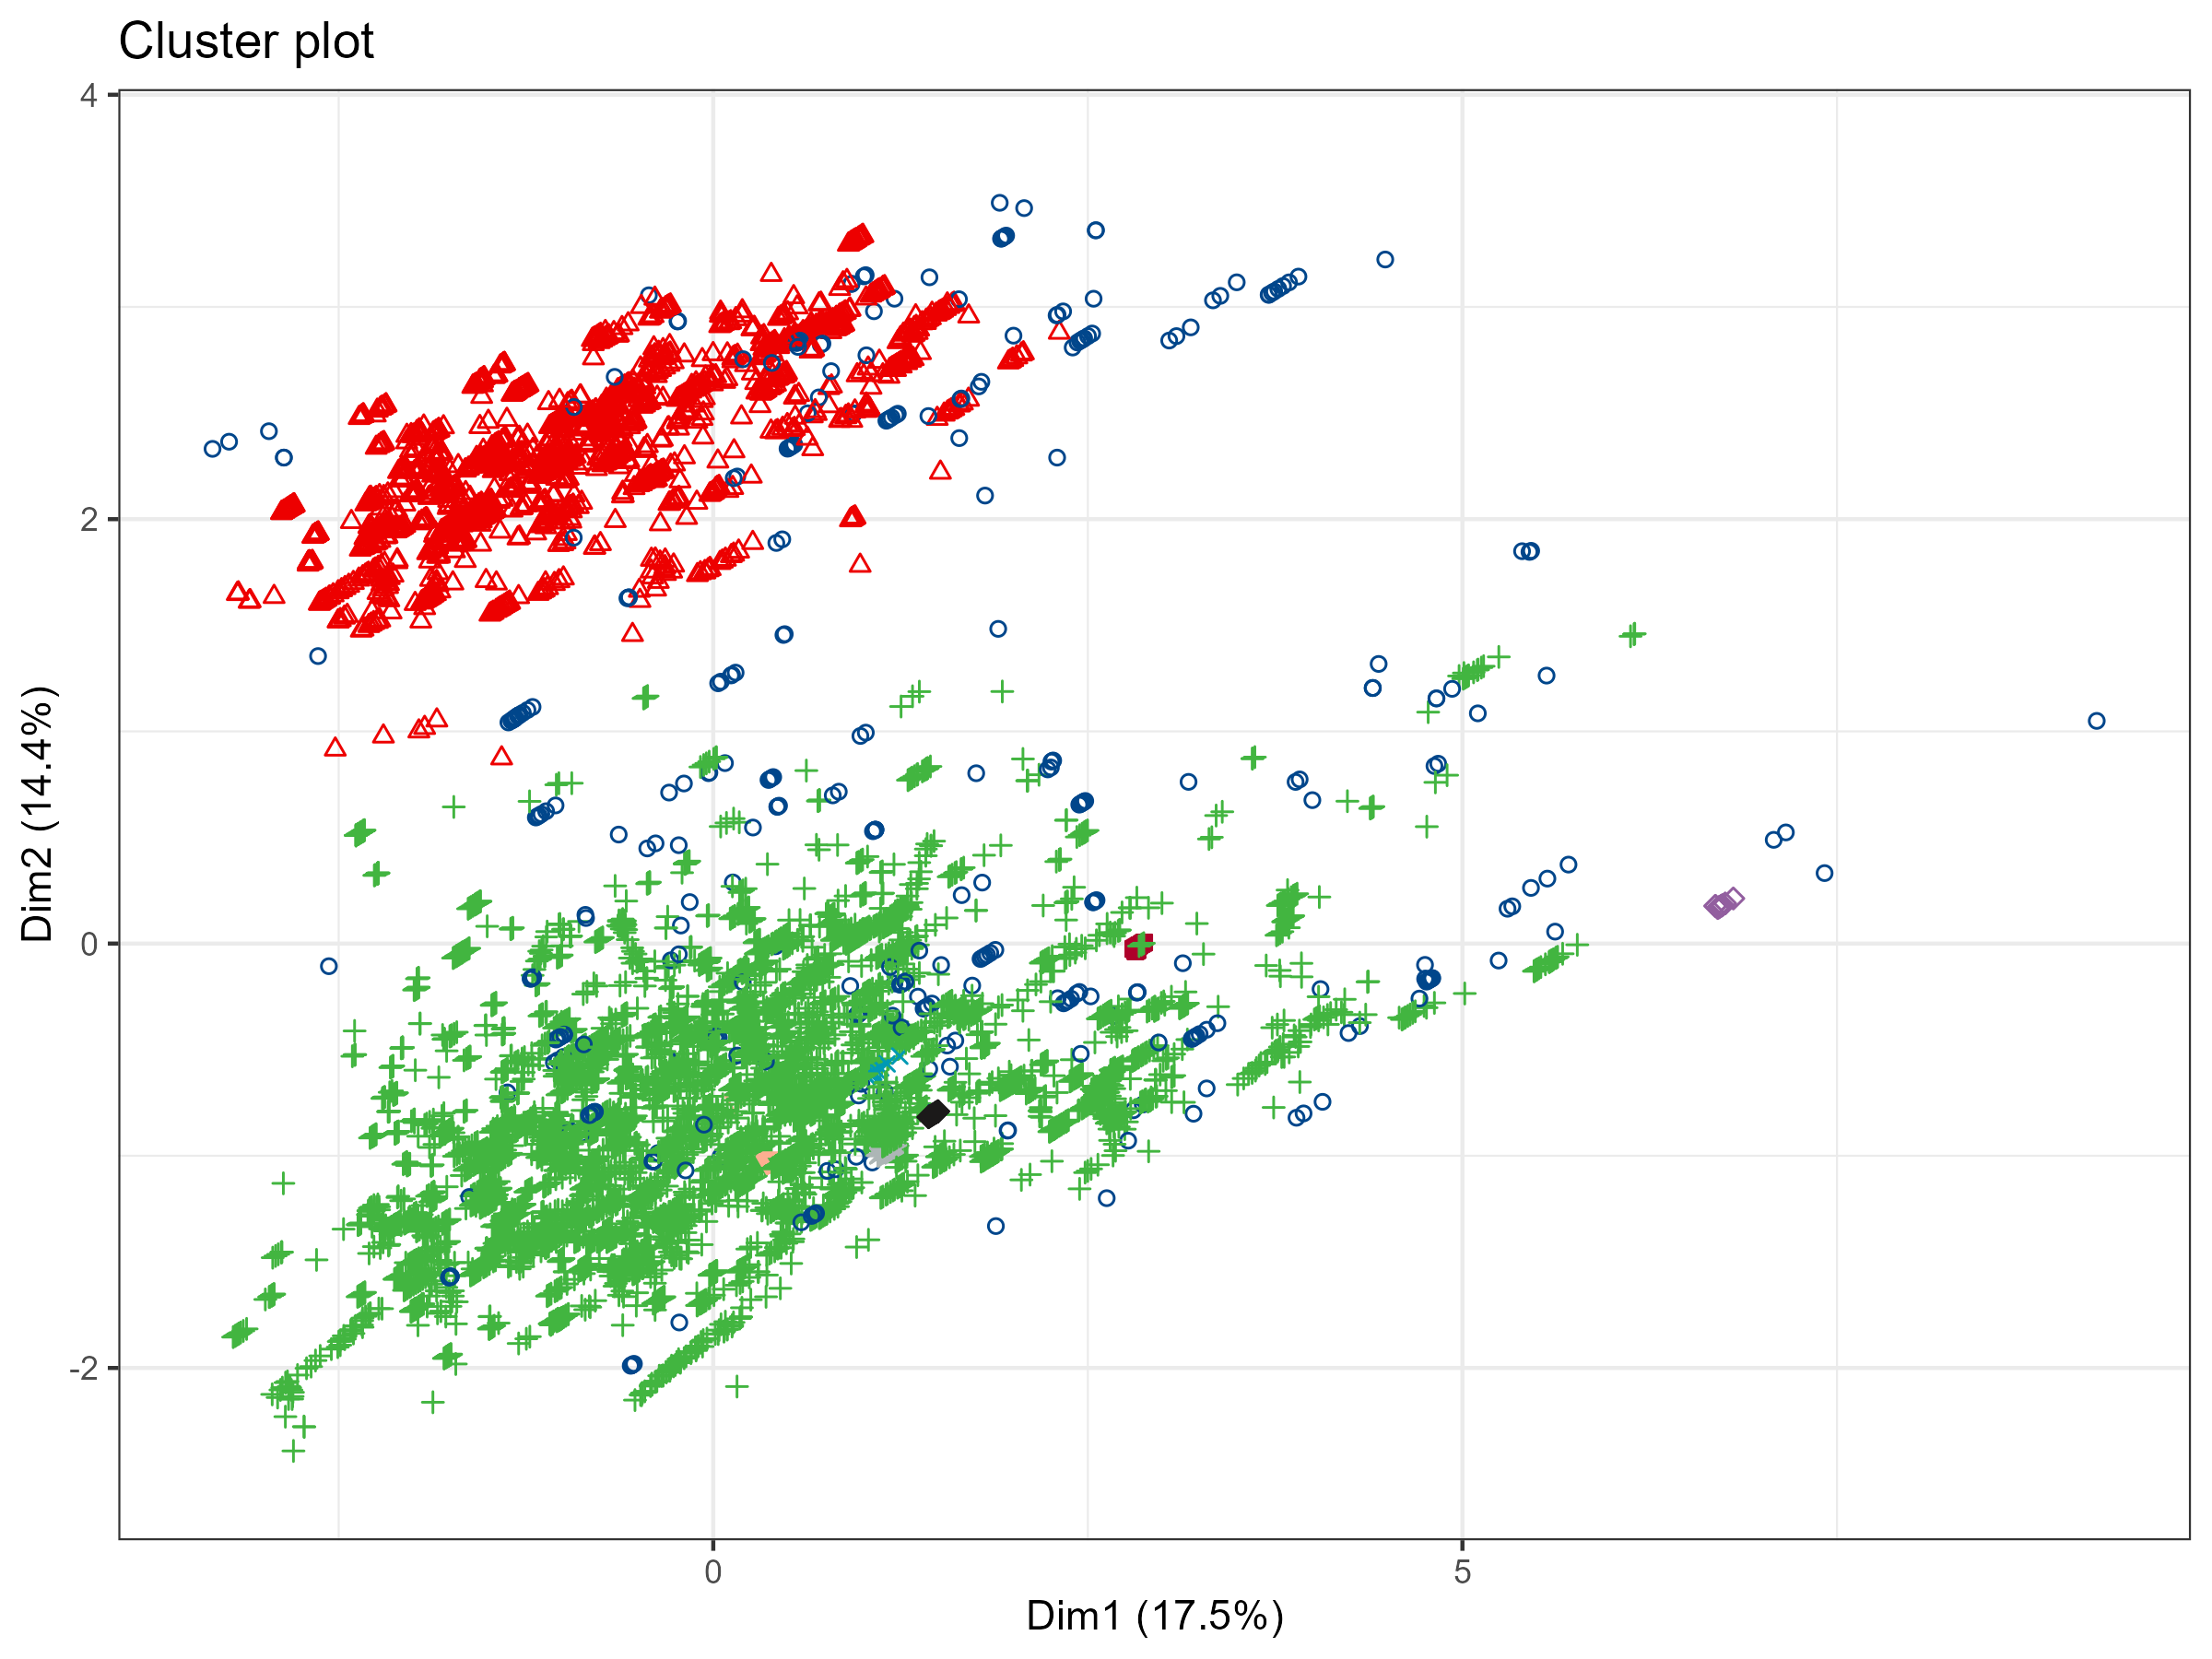
\includegraphics[width=0.8\textwidth]{Images/4_clustering/optics/opticsgrid.png}
    \caption{Resultats del clústering usant OPTICS, grid search (0.9, 10)}
    \label{fig:OPTICS_grid_res}
\end{figure}


S'observen dos clústers principals (tot i que realment n'hi ha uns 20). També veiem bastants outliers (en total 792) i clústers petits al sector dret, similar als que veiem amb el DBSCAN. L'alternativa a aquest gridSearch era usar el silhouette, però no dóna bons resultats en aquest cas, creant més de 300 clústers diferents (figura \ref{fig:OPTICS_silo}).
\begin{figure}[H]
    \centering
    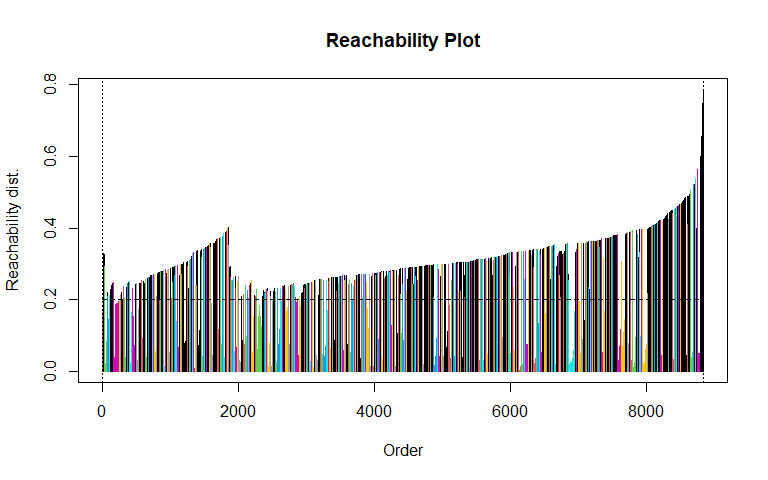
\includegraphics[width=0.8\textwidth]{Images/4_clustering/optics/siloreachability.png}
    \caption{Reachability de OPTICS usant silhouette (0.2, 22)}
    \label{fig:OPTICS_silo}
\end{figure}

En conclusió, sembla ser que l'optics no és una bona tècnica de clústering per aquestes dades. Com a molt, és capaç d'acostar-se als resultats obtinguts amb el DBSCAN. En general, les dues tècniques no han sigut capaces de crear clústers lo suficientment interessants i equilibrats com per poder extreure'n bona informació, o sigui que probablement no siguin les millors per aquestes dades. En aquest cas, el KMEANS creava uns clústers més interessants, i encara que no detectés outliers, probablement serien agrupacions més interessants.


\subsection{Clústering de sèries temporals}

S'ha realitzat una anàlisi de clústering de sèries temporals per a les cançons més escoltades mensualment a Spotify entre els anys 2017 i 2021. L'objectiu ha estat identificar patrons de comportament en les tendències de streams, que poden revelar agrupacions de cançons amb trajectòries similars en el temps, incloent hits ràpids o cançons amb una presència sostinguda en el temps.

Per dur a terme aquesta anàlisi, primer s'han carregat i preparat les dades, transformant-les per adequar-se a l'anàlisi de sèries temporals. Aquesta preparació ha inclòs la transformació de les variables \texttt{year\_week} i \texttt{month\_week} en una única columna de text per al mes i any, així com la pivotació de les dades per tenir aquesta nova variable \texttt{year\_month} en columnes i \texttt{track\_name} en files. Per a cada valor de fila i columna es va fer una agregació de totes les reproduccions de la cançó en aquell mes en concret.

S'ha seleccionat la variable \texttt{streams} per a l'anàlisi, considerant que aquesta proporcionaria el major benefici per a l'empresa al analitzar les cançons amb tendències de popularitat ràpida o sostinguda. S'ha prestat molta atenció al fet que, degut a que les dades només inclouen les cançons que estan dins del top 40 global de Spotify, les streams d'una cançó en un mes on no apareix cap vegada s'han considerat com a 0. Aquesta aproximació s'ha justificat amb l'ús de la Distància Temporal Dinàmica (DTW) per al càlcul de similituds, entenent que els valors 0 tenen menys pes en la comparació, i per tant, l'anàlisi es centra més en les tendències presents que en les absències.

Amb les dades preparades, s'ha realitzat un clústering jeràrquic utilitzant la distància DTW i el mètode de Ward. Aquest mètode s'ha escollit per la seva capacitat de crear grups basats en la minimització de la variància dins dels clústers, ideal per identificar grups de cançons amb patrons de streams similars al llarg del temps. 

Després de l'anàlisi jeràrquic, s'ha realitzat el dendrograma per poder escollir quin és el nombre més adequat de classes.

\begin{figure}[H]
    \centering
    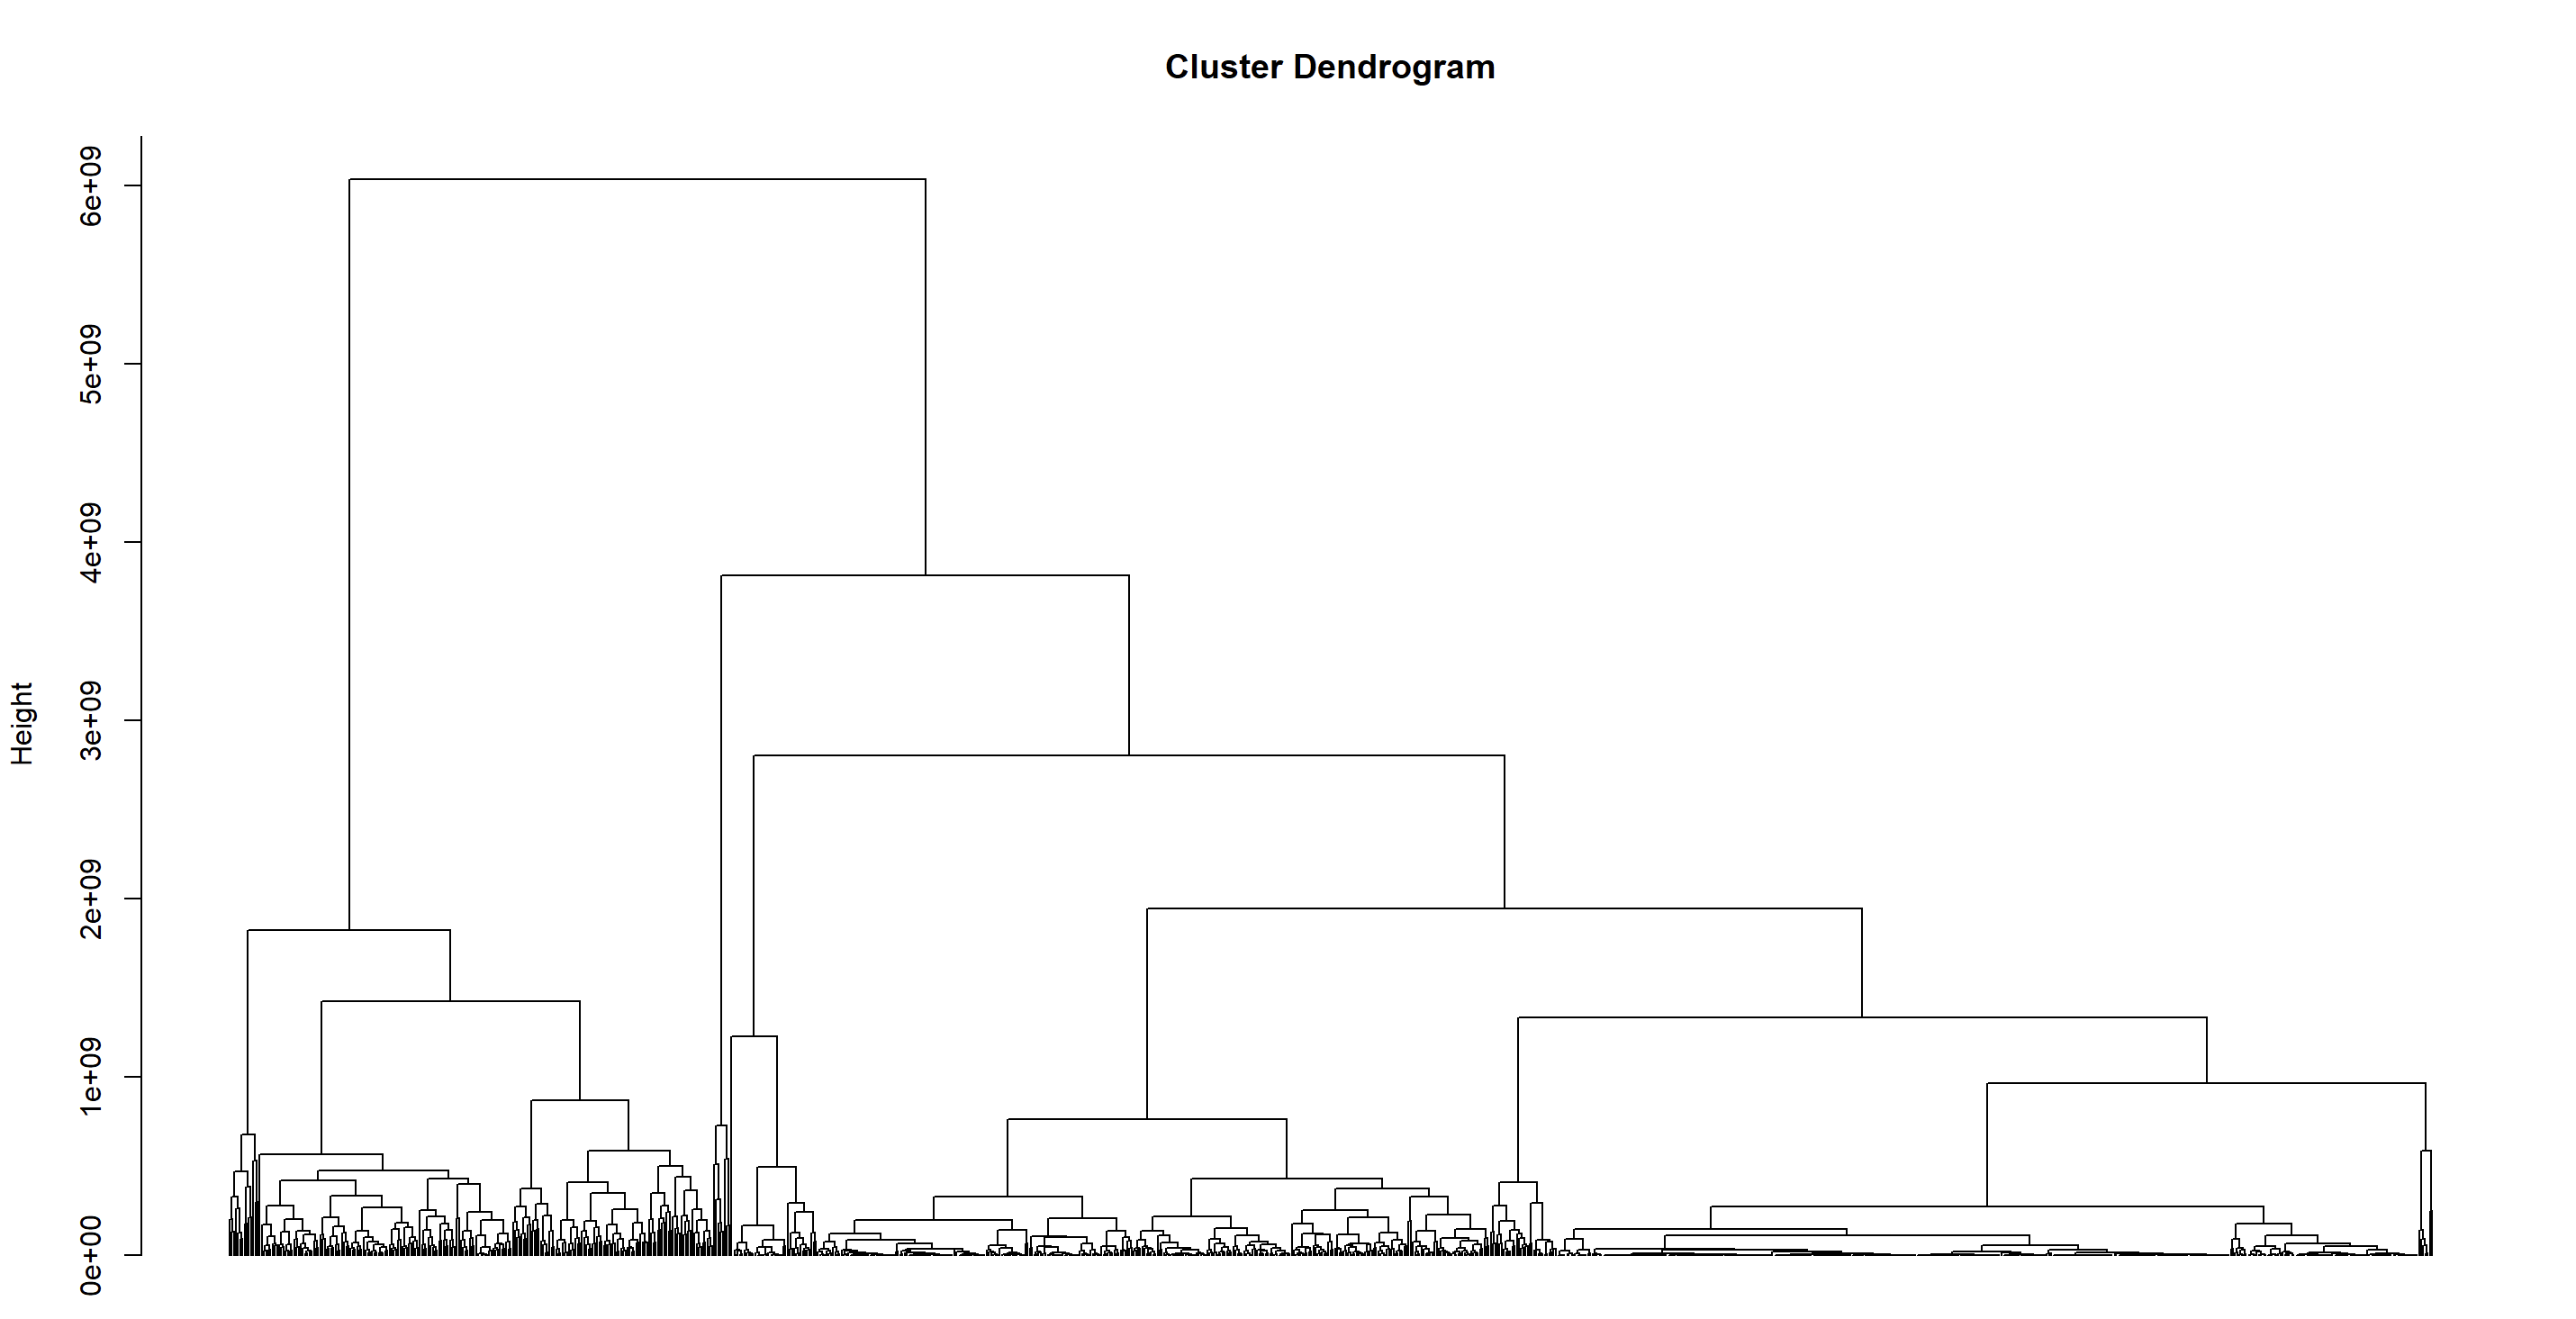
\includegraphics[width=\textwidth]{Images/4_clustering/time_series/dendrograma_original.png}
    \caption{Dendrograma de cançons utilitzant distància \texttt{DTW} i mètode \texttt{ward.D2}}
    \label{fig:TS_dendrograma_original}
\end{figure}

Com es pot veure en la figura \ref{fig:TS_dendrograma_original} el nombre \textit{k} a escollir no és gaire evident degut al desbalanceig de la majoria de clústers. Després d'analitzar aquest equilibri de classes, s'ha realitzat un tall per obtenir 5 classes diferents per tal d'intentar tenir una quantitat de cançons similar a tots els clústers (intentant mantenir una \textit{k} petita igualment).

Com es pot veure en la següent taula \ref{tab:TS_clustering_results} les 3 primeres classes tenen un nombre prou equilibrat de cançons mentre que en el quart n'hi ha moltes menys i en el cinquè gairebé no n'hi ha cap. Aquest fet és curiós degut a que molt probablement aquestes cançons agrupades en classes tan reduïdes podrien estar molt relacionades entre si podent arribar a conclusions interessants.

\begin{table}[H]
\centering
\begin{tabular}{|c|c|c|c|c|}
\hline
1    & 2    & 3   & 4   & 5 \\ \hline
311 & 436 & 224 & 40 & 8  \\ \hline
\end{tabular}
\caption{Resultat del clústering de les sèries temporals}
\label{tab:TS_clustering_results}
\end{table}

Una vegada s'ha escollit el valor de $k = 5$, en la figura \ref{fig:TS_dendrograma_colors} es pot veure el dendrograma colorejat per tal de visualitzar els diferents clústers. El color verd representa el clúster número 3, el color lila el 5, el blau el 4, el vermell l'1 i el mostassa el 2.

\begin{figure}[H]
    \centering
    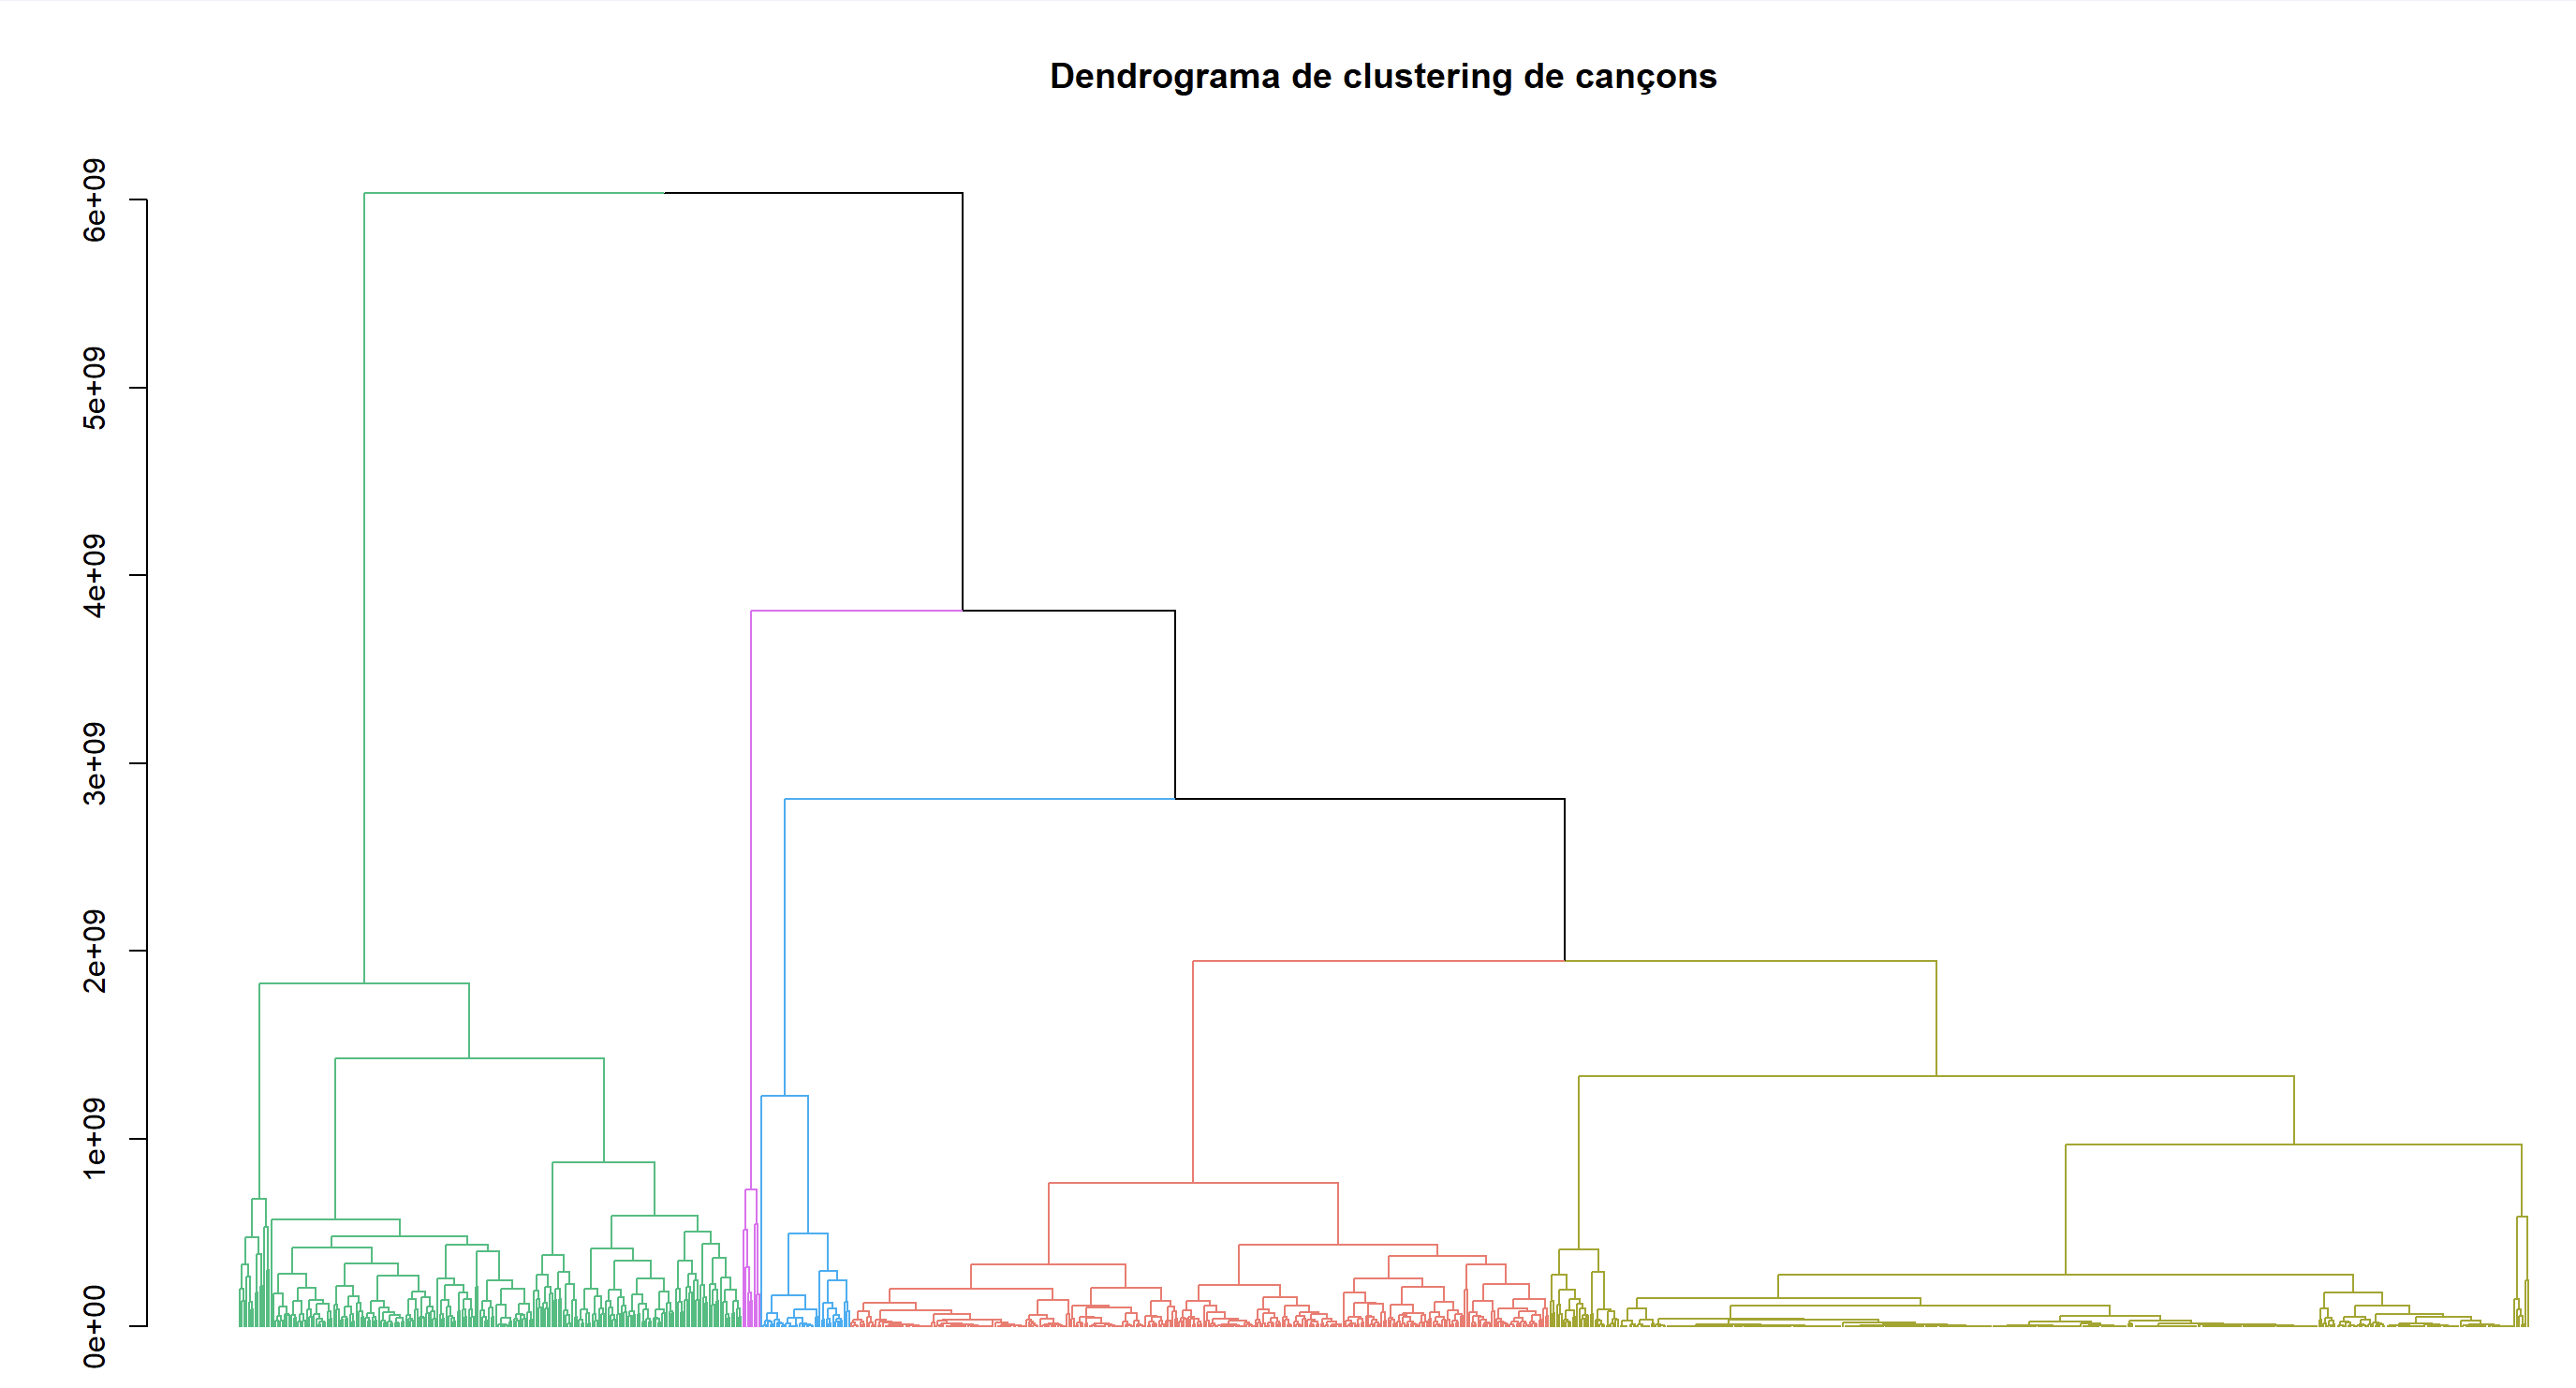
\includegraphics[width=\textwidth]{Images/4_clustering/time_series/dendrograma_colors.png}
    \caption{Dendrograma de cançons utilitzant distància \texttt{DTW} i mètode \texttt{ward.D2} amb els clústers colorejats ($k = 5$)}
    \label{fig:TS_dendrograma_colors}
\end{figure}

\subsubsection{Anàlisi dels resultats}

Amb els clústers ja establerts, s'ha procedit a realitzar un anàlisi detallat dels resultats amb l'objectiu d'interpretar i comprendre els motius subjacents que han conduït a la formació d'aquestes agrupacions

Les visualitzacions i anàlisis post-clústering, com ara la comparació entre els clústers i la durada mitjana de les cançons per cada agrupació, ofereixen una perspectiva més profunda permetent descobrir patrons amagats que ajudin a entendre millor la situació musical de l'aplicació.

Pel que fa a la figura \ref{fig:TS_tsclust_sc} podem observar les evolucions de les reproduccions per a cada clúster al llarg del temps.  Simplement al fer una breu ullada ja podem veure, més o menys, com estan distribuïdes les cançons. \\

\begin{itemize}
    \item \textbf{Clúster 1:} Aquest grup mostra un patró consistent en la quantitat de \textit{streams} amb un alt nivell de superposició de les sèries alhora que allargada, indicant una quantitat de streams sostinguda.
    
    \item \textbf{Clúster 2:} Aquest clúster presenta uns pics molt marcats al llarg dels anys indicant èxit ocasionalment que podria ser a causa de promocions o esdeveniments o inclús d'altres aplicacions que tenen molt poder d'influència com ara \textit{TikTok}. Cal recordar que la majoria de cançons es troben en aquest grup, i en aquests pics no s'hi veuen moltes cançons, de manera que hi ha una gran quantitat de cançons (les que no formen els pics) que no són tan populars i conformen la majoria del clúster.
    
    \item \textbf{Clúster 3:} Aquesta classe és molt similar al primer clúster però amb una diferència més significativa en les variacions entre cançons, encara que segueixen tenint una popularitat allargada. A més, els valors màxims són considerablement més alts que els del clúster 1, de manera que segurament hi ha cançons més populars en aquest clúster.
    
    \item \textbf{Clúster 4:} En aquest grup trobem les cançons que eren populars a l'inici de la creació del \textit{dataset} però que ràpidament van perdre l'interès, possiblement \textit{hits} d'aquella temporada. Cal mencionar com ja s'ha vist anteriorment que aquest clúster compta amb molt poques cançons, concretament 40.
    
    \item \textbf{Clúster 5:} Aquest grup, que és el més petit de tots, és el que té un període més llarg d'èxit i on les cançons tarden més en sortir del top després del pic. A més, els valors màxims són molt alts, de manera que segurament conté cançons molt populars.
\end{itemize}


\begin{figure}[H]
    \centering
    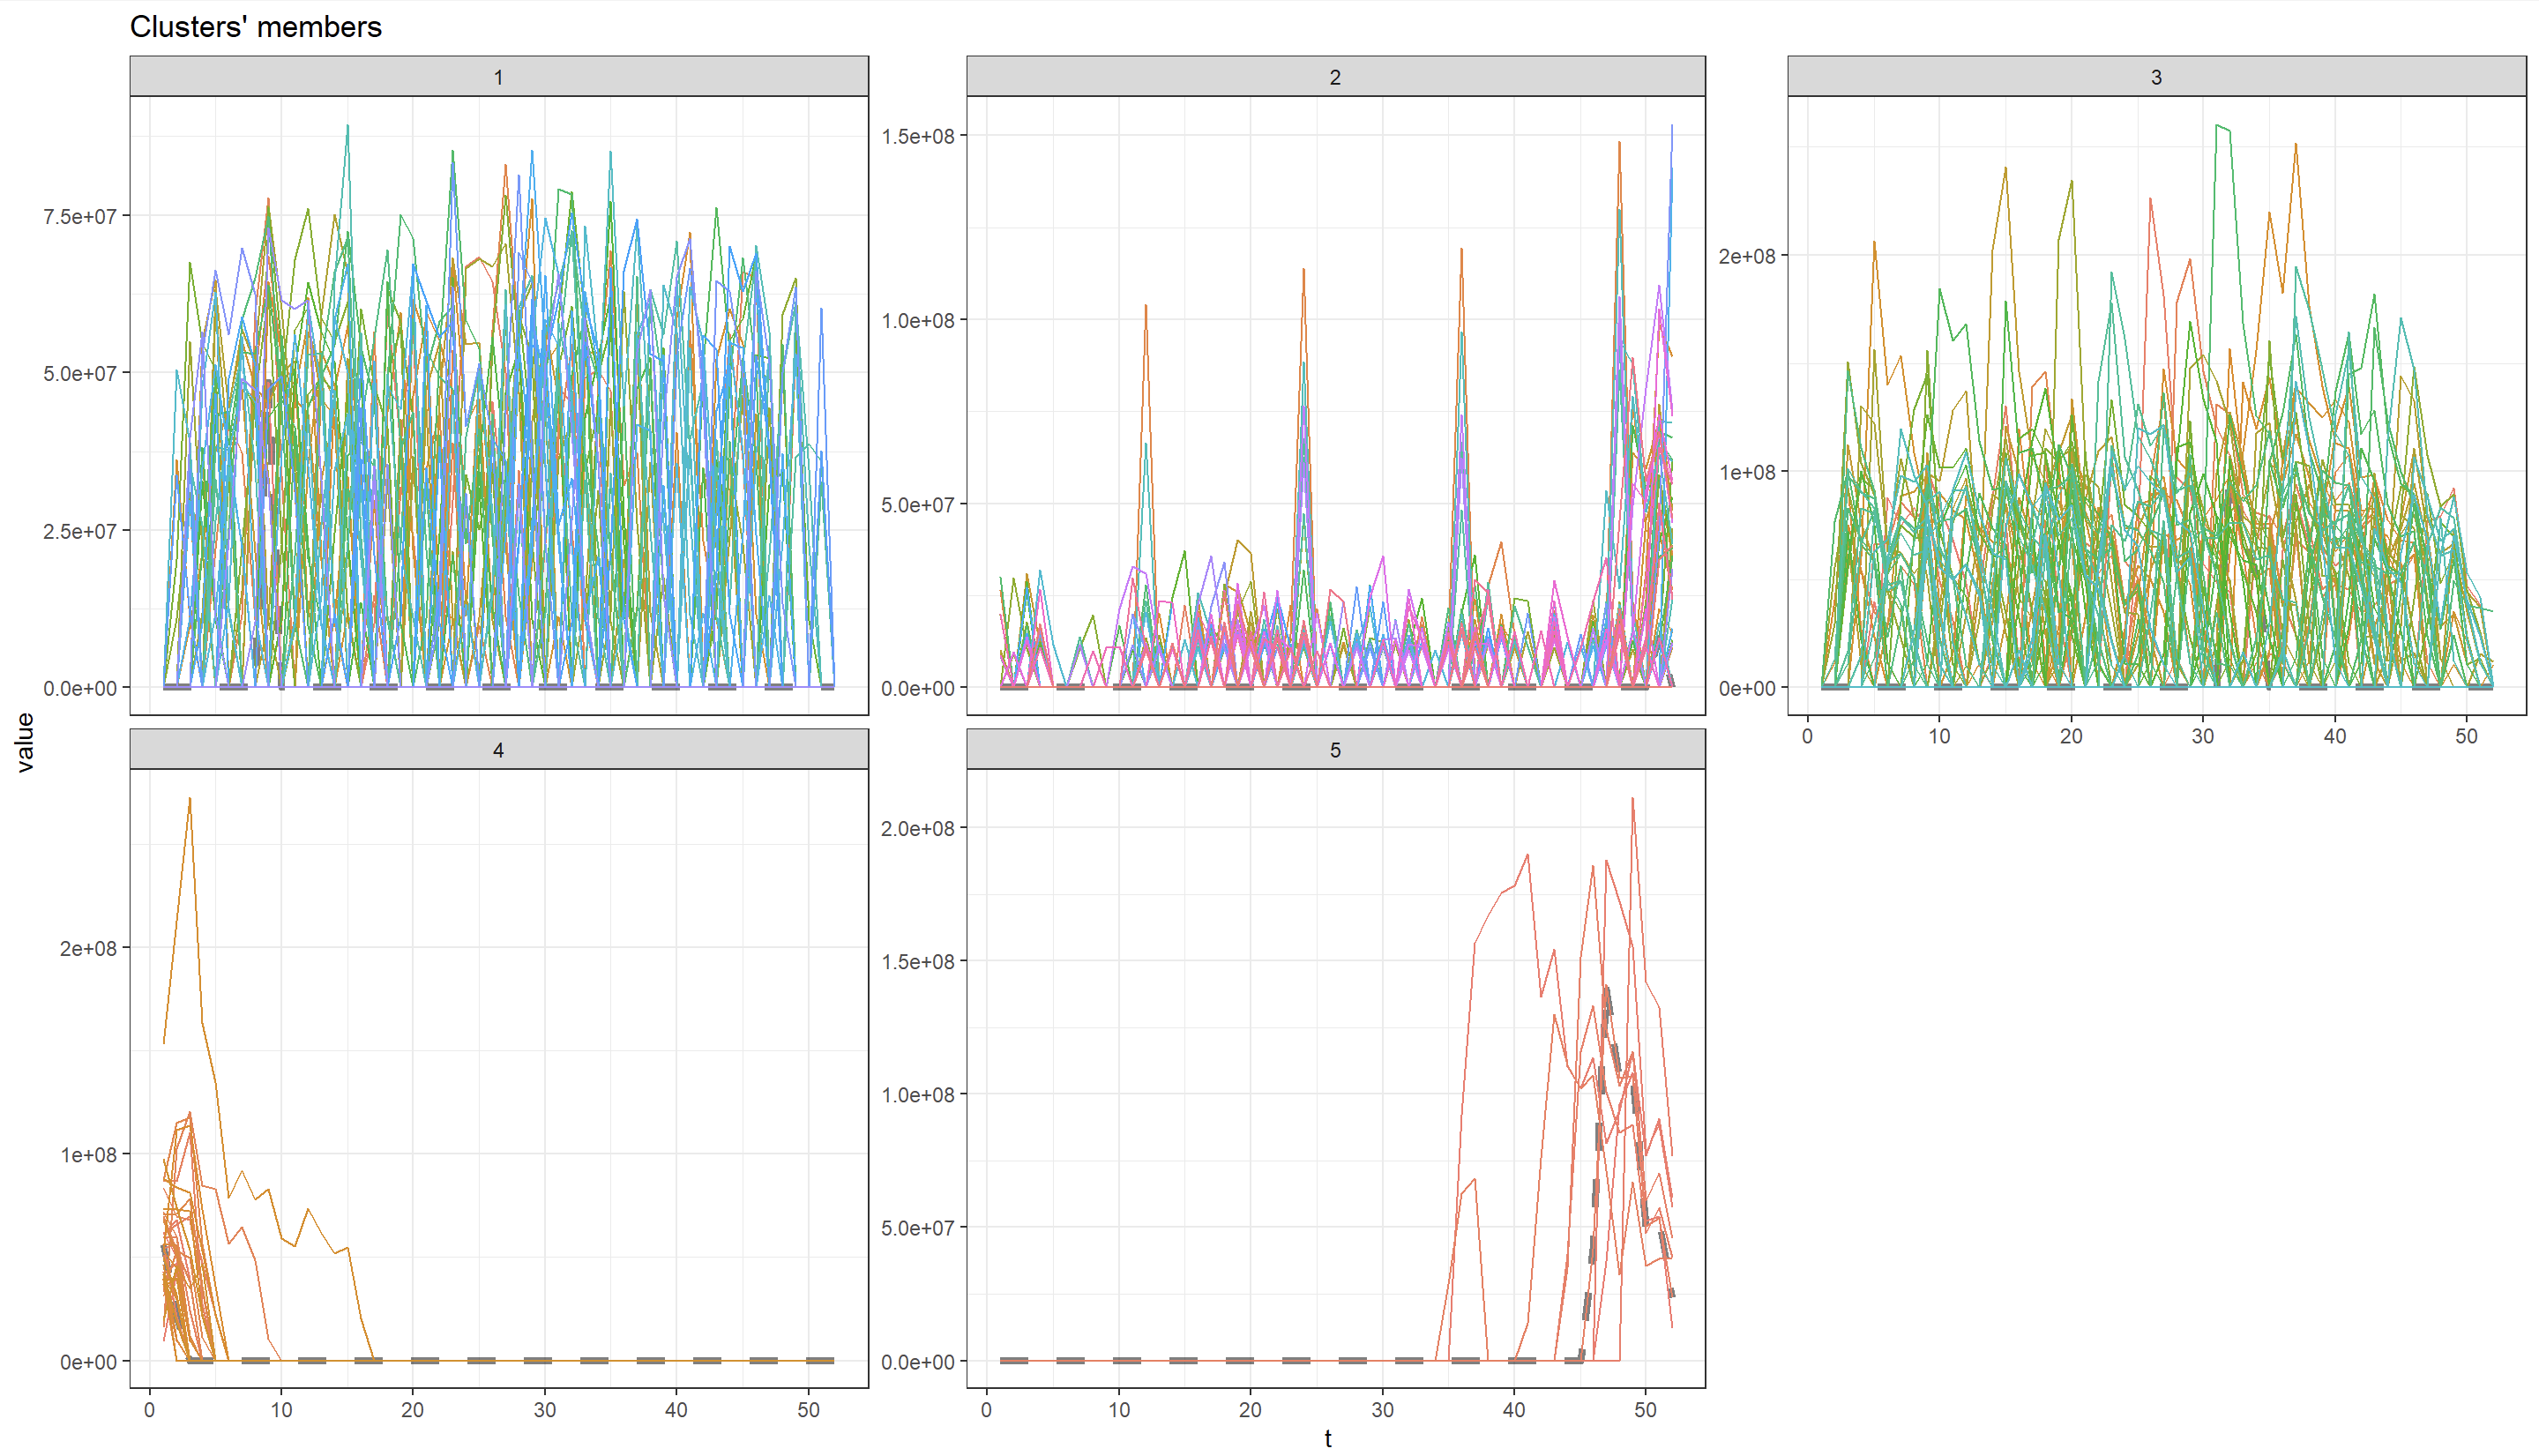
\includegraphics[width=0.8\textwidth]{Images/4_clustering/time_series/tsclust_sc.png}
    \caption{Gràfics de \textit{tsclust} amb l'evolució de streams per cada clúster}
    \label{fig:TS_tsclust_sc}
\end{figure}


Per poder acabar de visualitzar millor les conclusions anteriors s'ha creat un \textit{plot} per a cada classe representant l'evolució dels streams mensuals per cançó. Com podem veure en la figura \ref{fig:ts_clust_streams_month_cluster}, és molt similar a l'anterior però ens permet entendre millor les distribucions de les sèries. 

Tal i com s'ha mencionat, es pot mencionar que la diferència principal entre els clústers 1 i 3 és que aquests últims són bastant més populars alhora que la variància de streams és major entre cançons. També podem confirmar els forts pics espontanis del grup 2 i la major durada i gran popularitat de l'últim clúster (el 5).

A més, es pot veure com el clúster 3 (que conté les cançons que són generalment més populars) té una falta de cançons a l'inici i al final de la línia temporal. Això sembla justificar que el clúster 4 (amb nivells de popularitat semblants al grup 3) és el que conté les primeres cançons que haurien d'anar al clúster 3 (segurament separades pel fet de que han estat ``tallades'' per l'inici de la línia temporal, de manera que la seva sèrie temporal té una forma diferent); mentre que les cançons del clúster 5 semblen ser les cançons populars que haurien de correspondre al clúster 3, i les menys populars semblen haver anat al clúster 2 (degut a l'increment de reproduccions en aquest clúster al final de la seva línia temporal).

\begin{figure}[H]
    \centering
    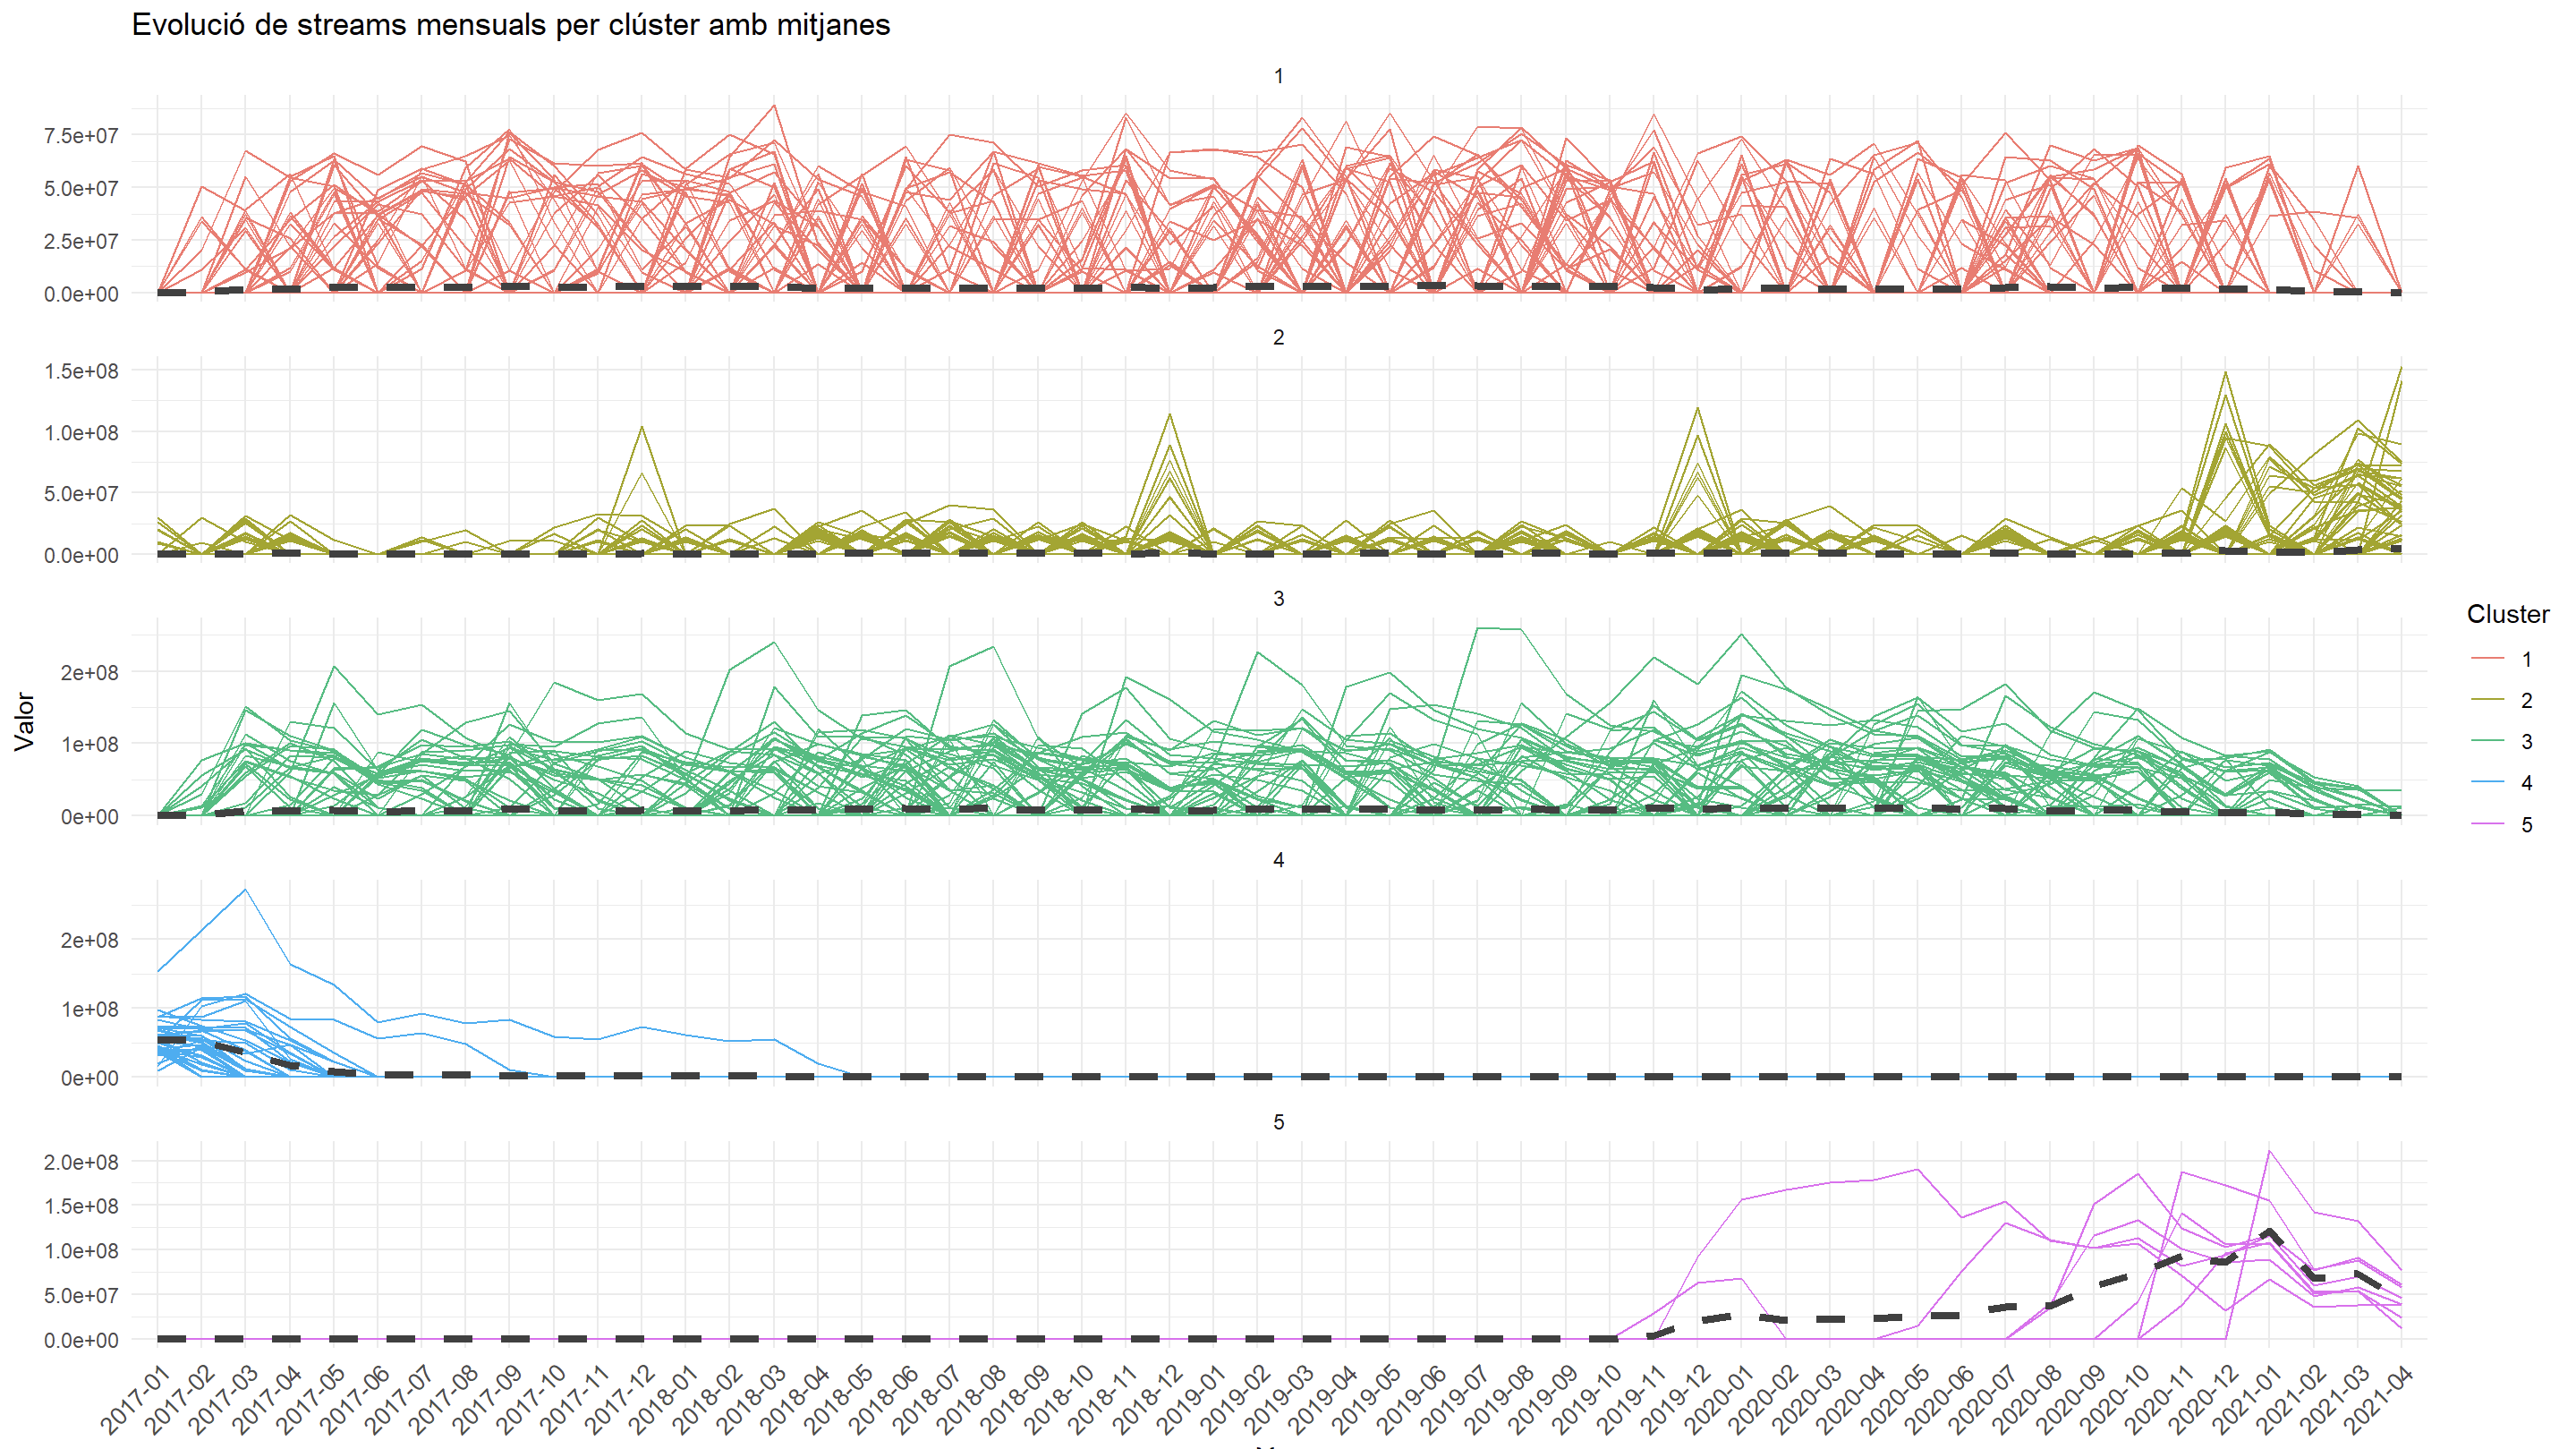
\includegraphics[width=0.8\textwidth]{Images/4_clustering/time_series/streams_cada_mes_per_cluster_amb_mitjana.png}
    \caption{Gràfics de l'evolució de les streams per a cada cançó dins de cada clúster}
    \label{fig:ts_clust_streams_month_cluster}
\end{figure}

Després d'analitzar aquestes sèries s'ha considerat important seguir l'estudi observant la mitjana de mesos actius de les cançons de cada grup indicant-nos així quins clústers contenen els èxits més prolongats i confirmant les conclusions anteriors.

En el primer \textit{barplot} \ref{fig:TS_barplot_mitjanes_mesos_actius} mostra la mitjana de mesos actius per clúster on es pot observar que el clúster 5, que és el més petit, conté les cançons que mantenen la popularitat constant durant el període de temps més llarg. El segon clúster que compleix això és el 3, com ja s'havia observat en l'anàlisi previ. 

Si ens fixem en el \textit{boxplot} \ref{fig:TS_boxplot_mesos_actius} podem observar i confirmar l'espontaneïtat de la classe 2 on pràcticament totes les cançons duren un sol mes en el top, encara s'hi poden observar \textit{outliers}.

\begin{figure}[H]
    \centering
    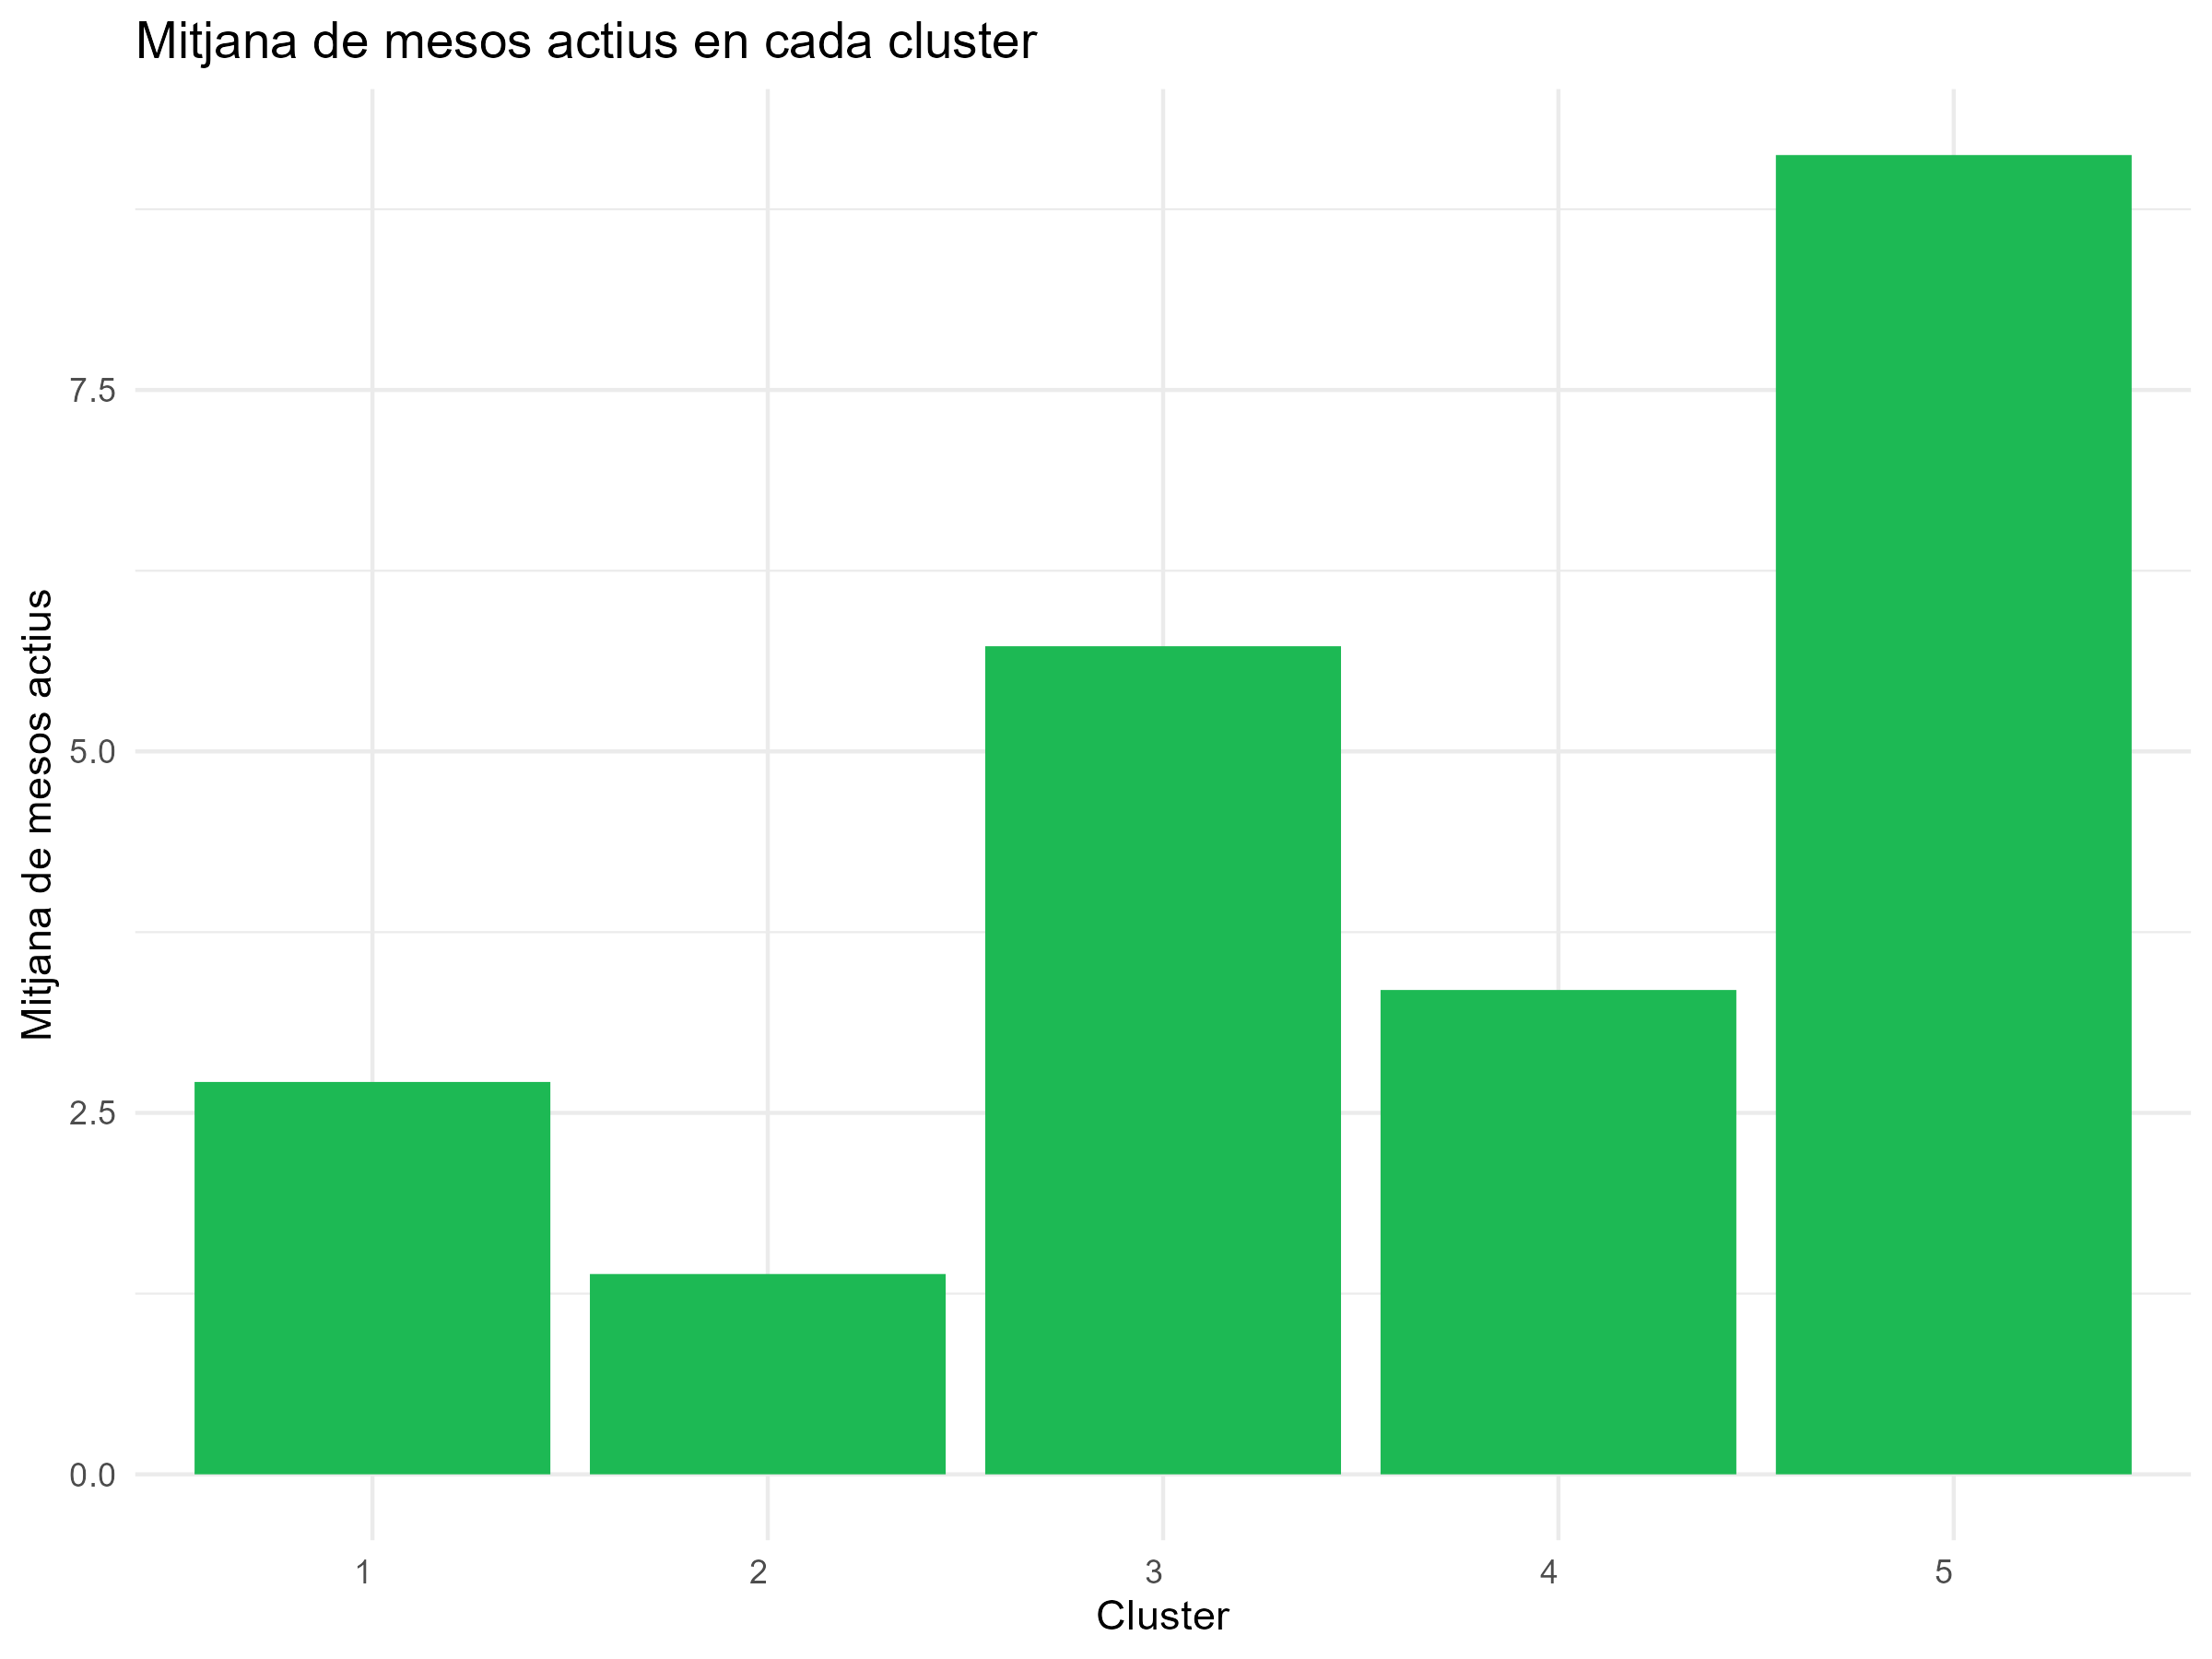
\includegraphics[width=0.8\textwidth]{Images/4_clustering/time_series/barplot_mitjanes_mesos_actius.png}
    \caption{Barplot de la mitjana de mesos actius de les cançons per cada clúster}
    \label{fig:TS_barplot_mitjanes_mesos_actius}
\end{figure}

\begin{figure}[H]
    \centering
    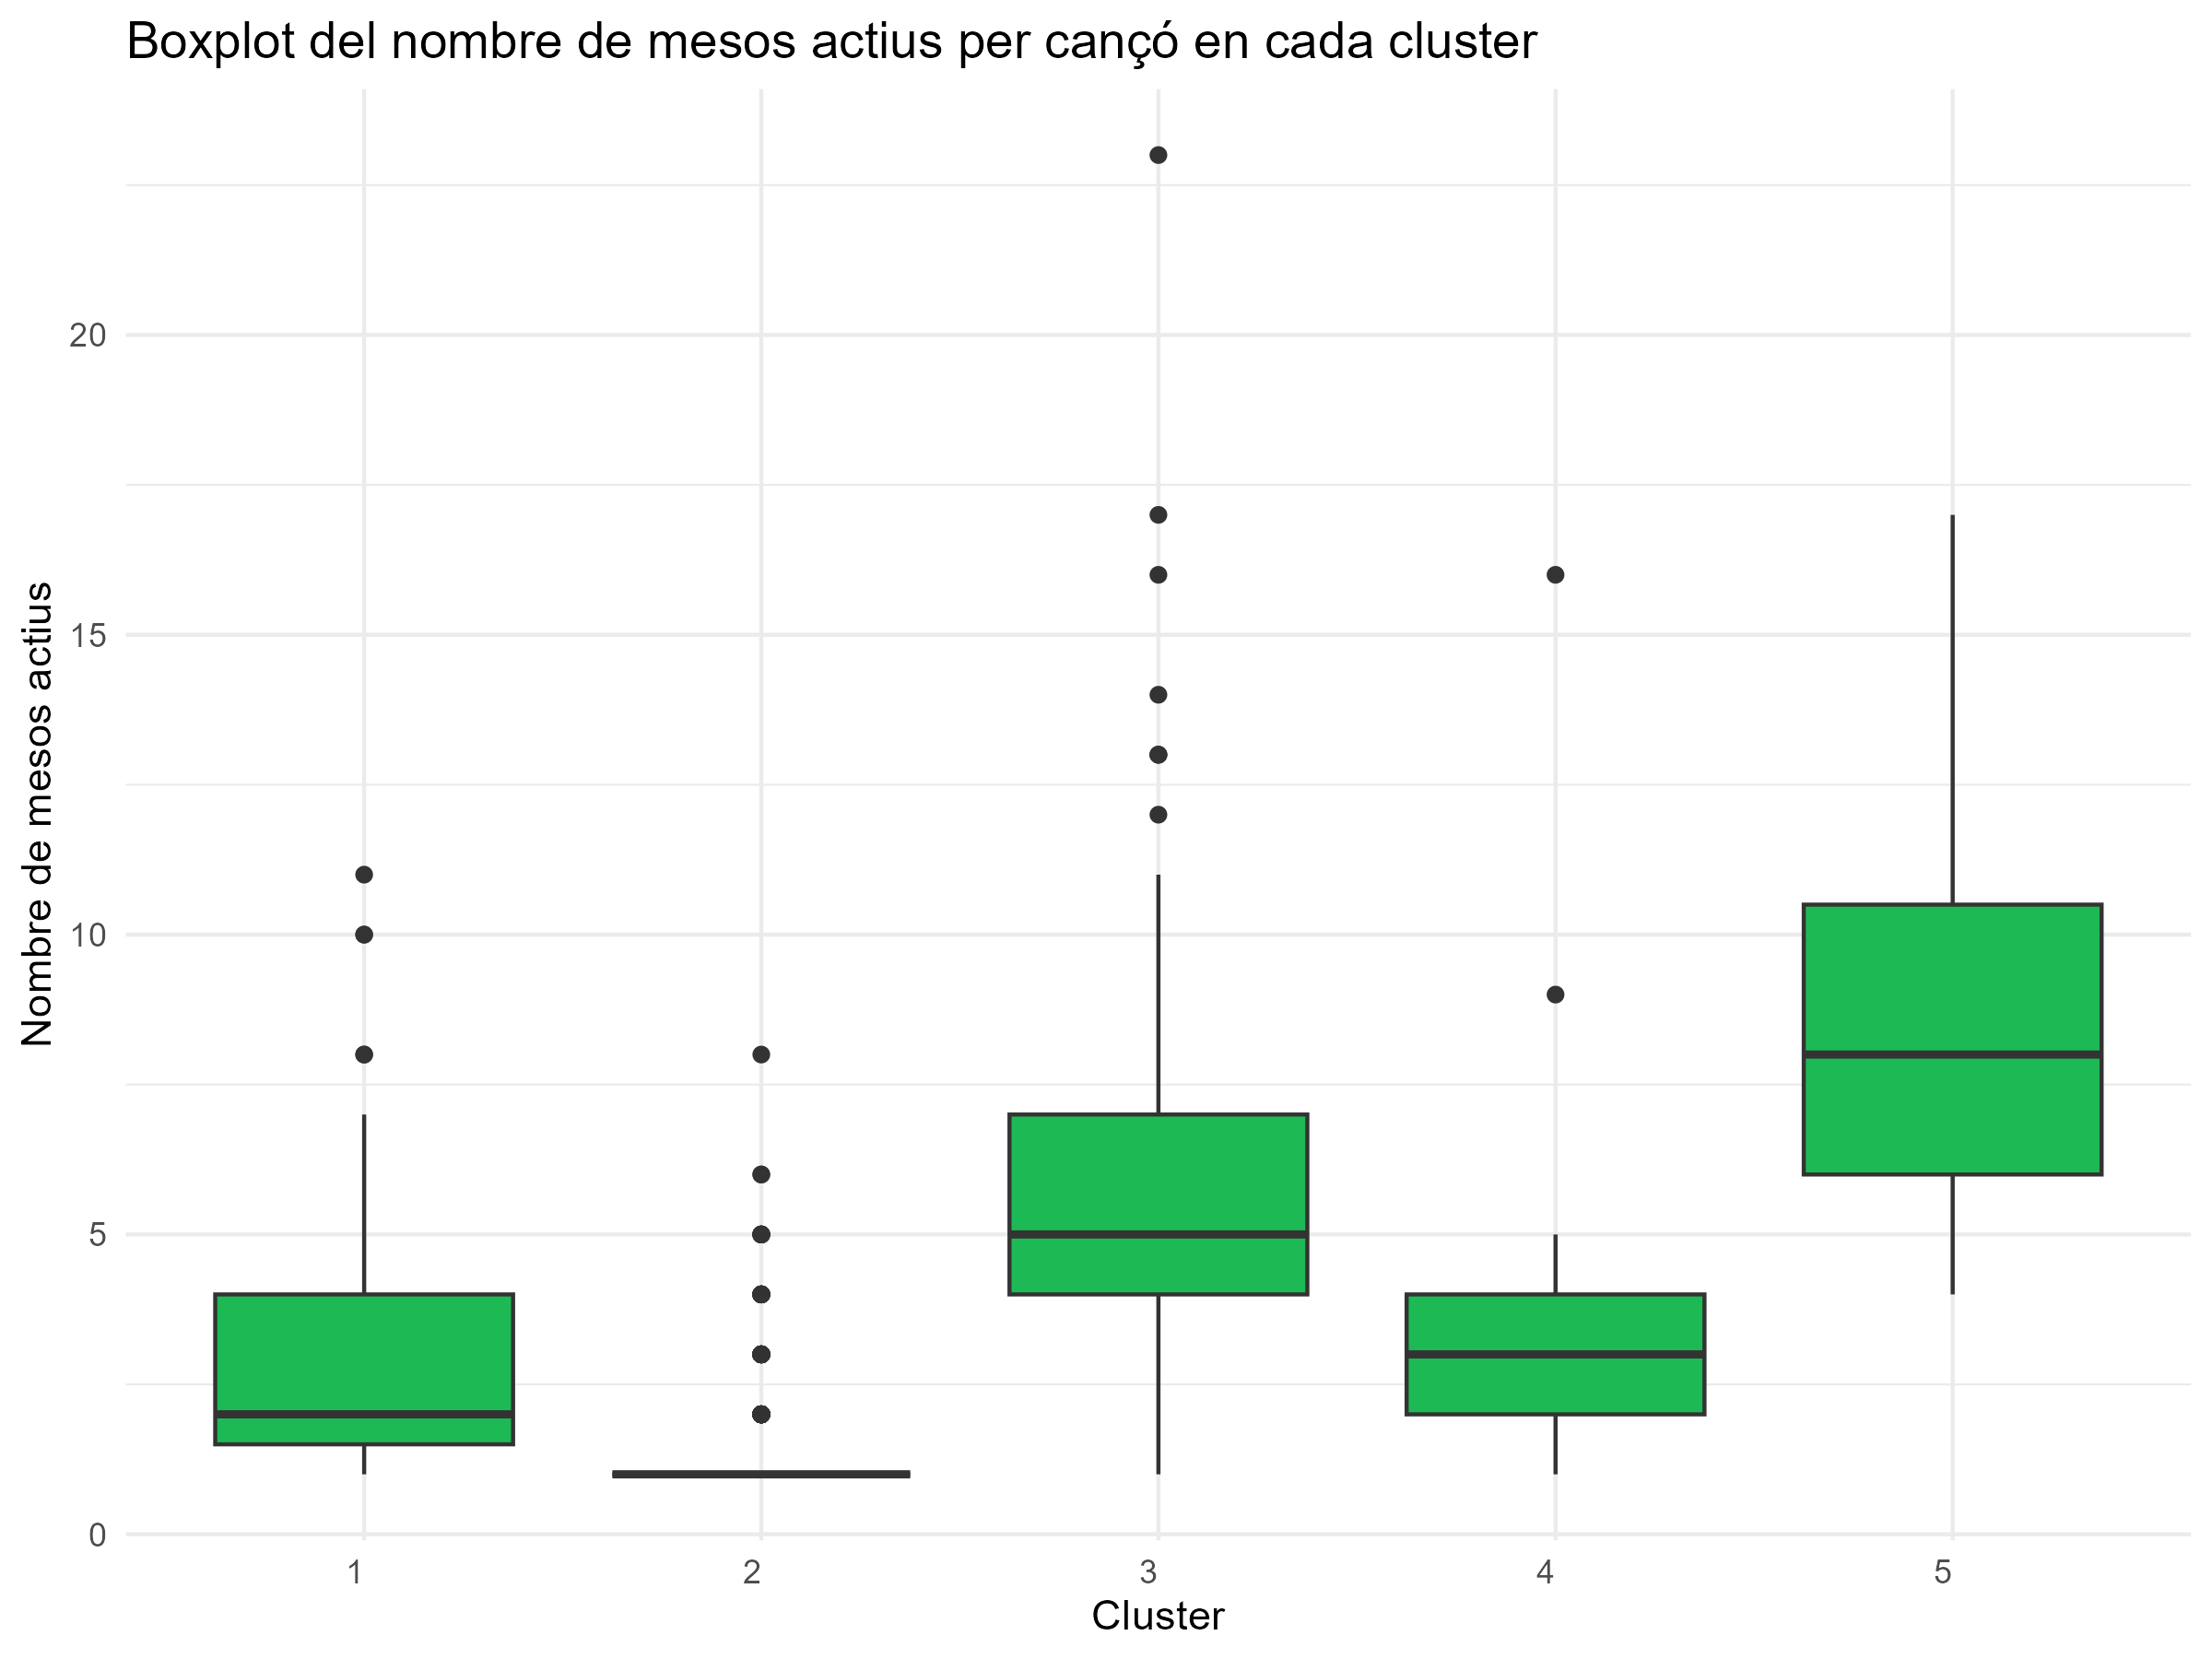
\includegraphics[width=0.8\textwidth]{Images/4_clustering/time_series/boxplot_mesos_actius.png}
    \caption{Boxplot de la distribució de mesos actius de les cançons per cada clúster}
    \label{fig:TS_boxplot_mesos_actius}
\end{figure}

Per poder comprendre millor els clústers, s'ha realitzat un gràfic agrupat per mesos per poder veure si hi ha algun patró estacional ens els diferents clústers. Com es pot veure en la figura \ref{fig:TS_evol_streams_per_mes_i_cluster}, aparentment en els 3 primers clústers no hi ha gaire diferència entre mesos, tan sols es podria comentar un lleuger augment de reproduccions durant els mesos d'estiu.

Pel que fa als clústers 4 i 5, com ja s'ha mencionat prèviament corresponen a les cançons que inicien i acaben els tops en el dataset. Com que els primers valors es van mesurar al gener de 2017, podem veure que en el clúster número 4 (color blau) durant els primers mesos de l'any té moltes streams però a partir del juny ja pràcticament no en té. Per altra banda, el clúster 5, concentra els seus streams durant els mesos d'hivern, ja que és quan hi ha els últims valors mesurats del dataset.

\begin{figure}[H]
    \centering
    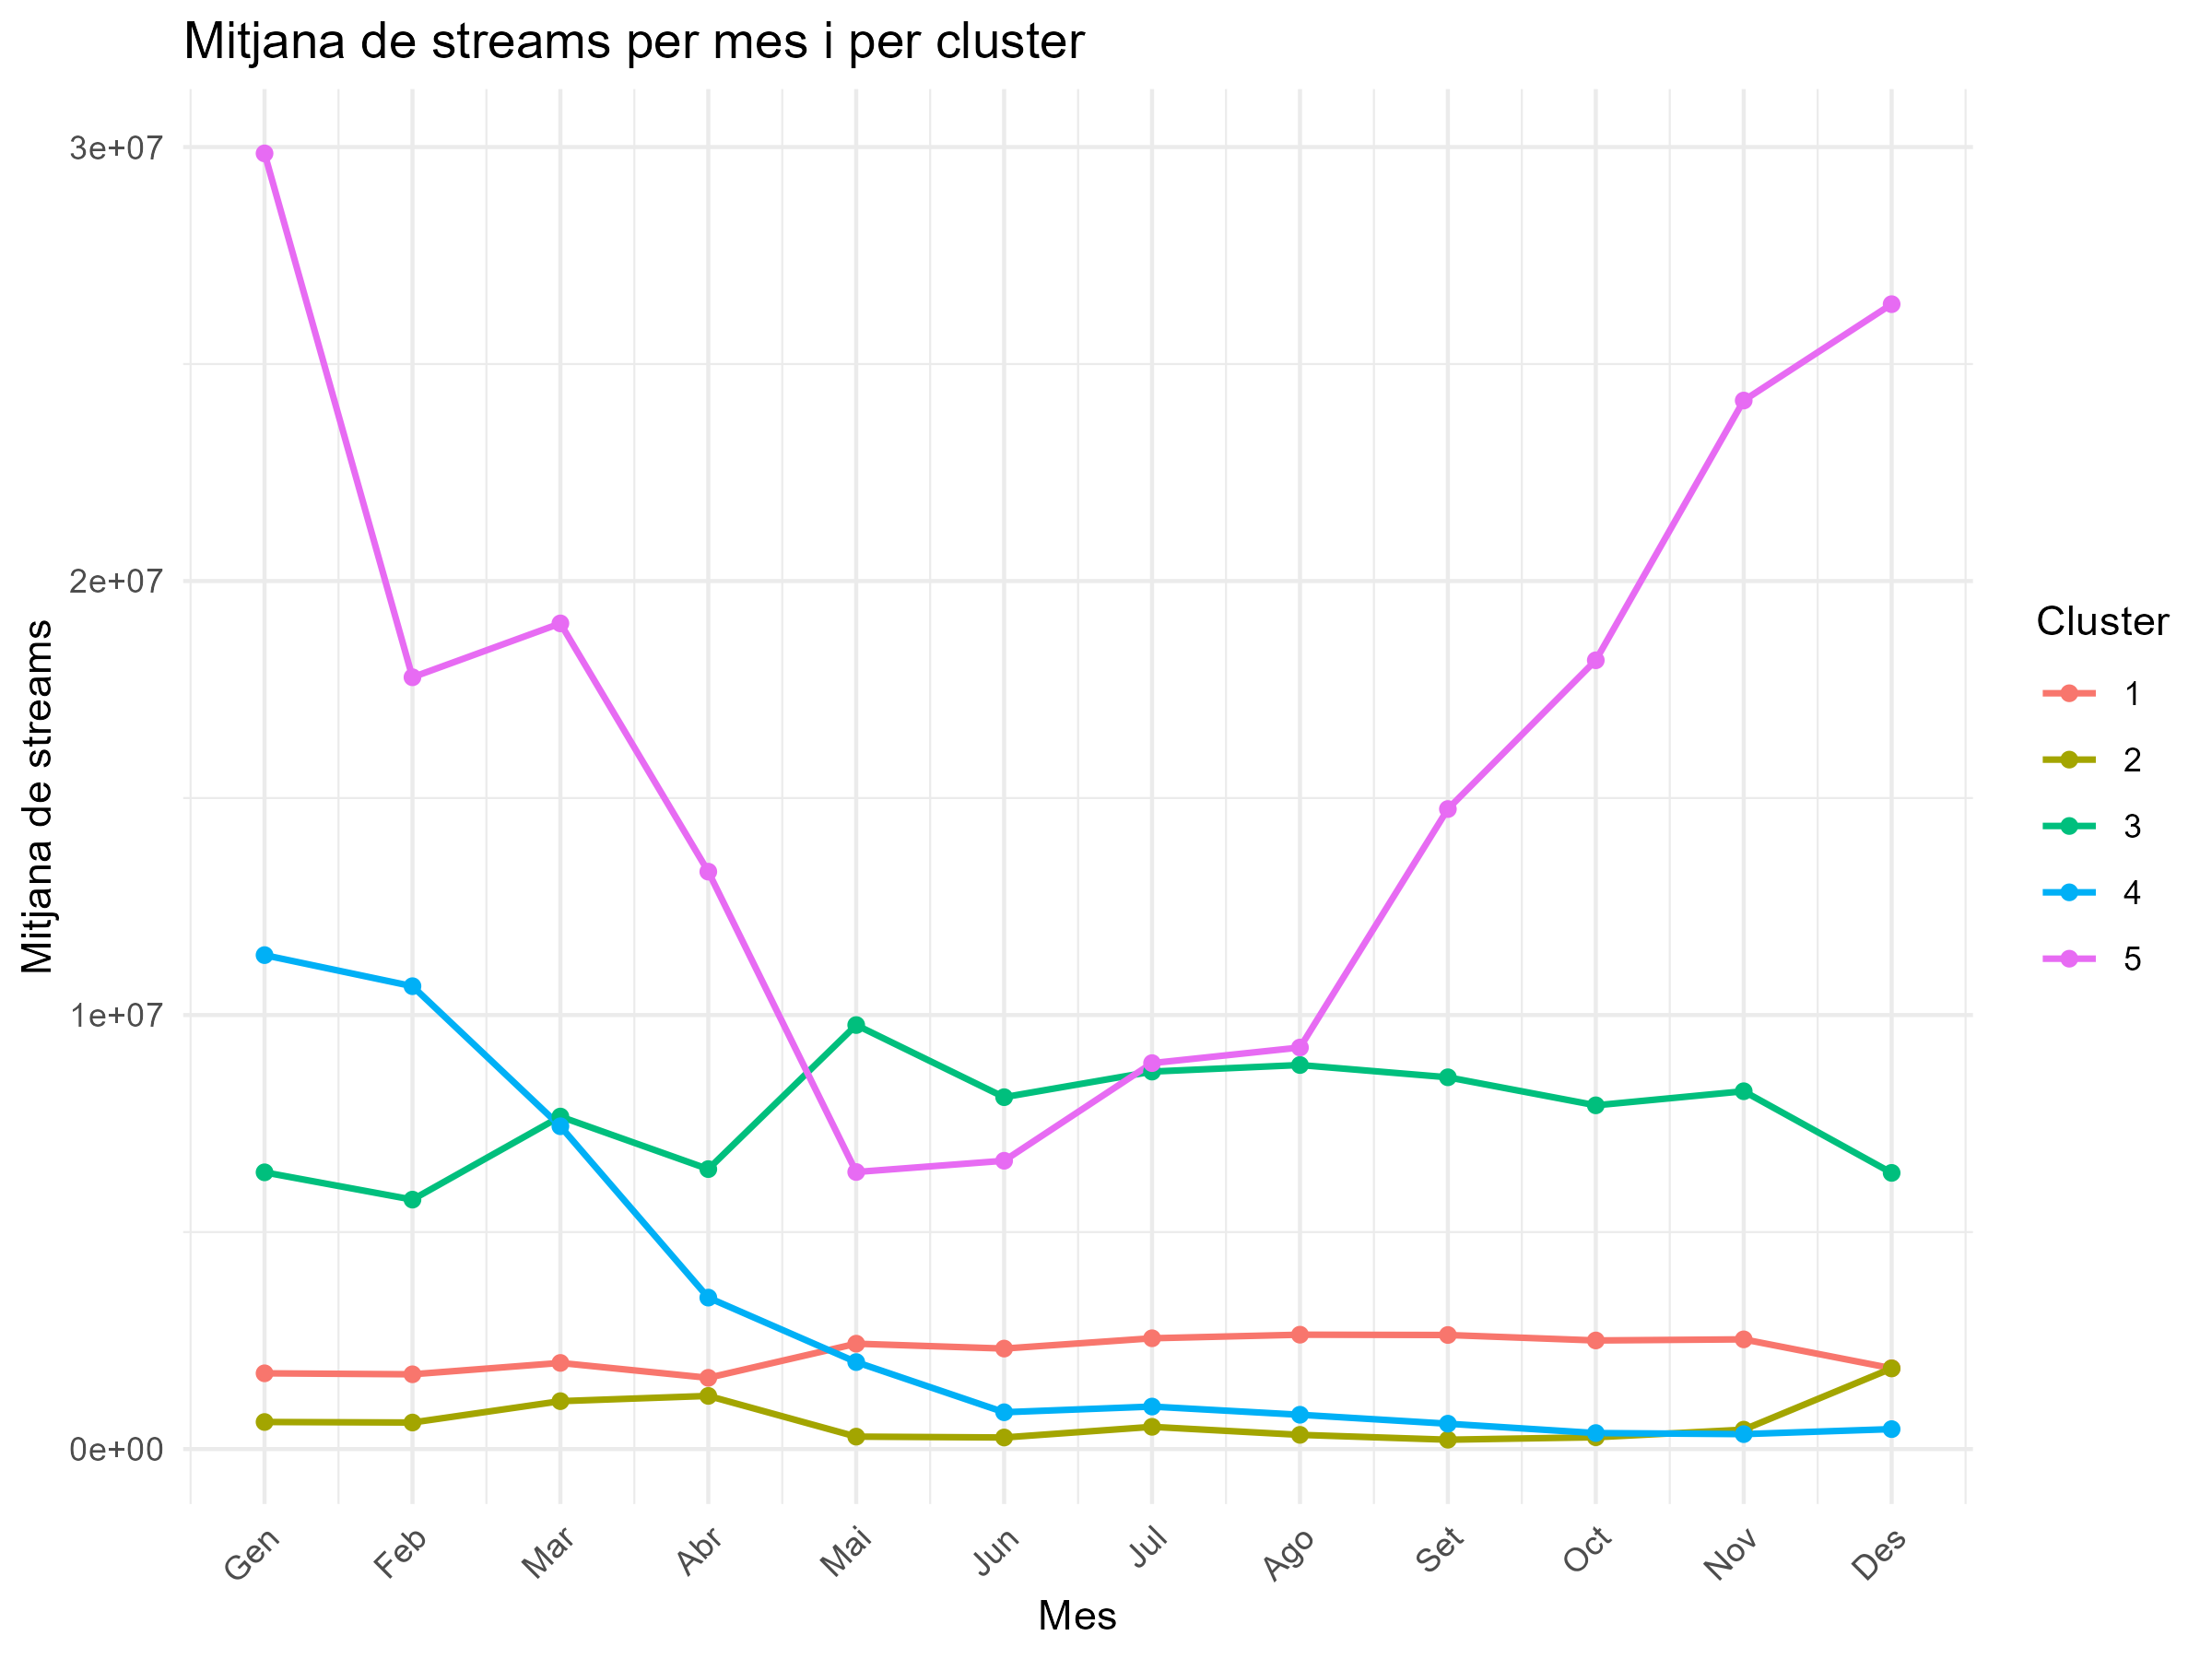
\includegraphics[width=0.8\textwidth]{Images/4_clustering/time_series/evol_streams_per_mes_i_cluster.png}
    \caption{Gràfic amb la mitjana dels streams de cada clúster en funció dels mesos}
    \label{fig:TS_evol_streams_per_mes_i_cluster}
\end{figure}

Com s'ha mencionat prèviament, quan una cançó no apareix en el top 40 durant tot el mes, el seu valor de streams s'ha considerat 0. Això implica que en el gràfic de la figura \ref{fig:TS_evol_streams_per_mes_i_cluster} les mitjanes inclouen molts zeros, de manera que els resultats poden estar condicionats per la quantitat de mesos actius de cada clúster (que ja s'ha vist prèviament). Per tal de veure l'evolució de les mitjanes de streams al llarg dels mesos només tenint en compte quan les cançons estan al top 40 (sense considerar els zeros) s'ha creat el gràfic de la figura \ref{fig:TS_evol_streams_per_mes_i_cluster_no_zeros}. Com es pot veure, el canvi és important, i ara s'aprecia com, per exemple, el clúster 2 té un increment de streams en el mes de desembre (tal i com es veia en els pics mencionats prèviament), però durant tot i així té una mitjana de streams baixa al llarg de tot l'any. Pel que fa al clúster 1, és el més estable de tots i no conté cançons gaire populars. Per altra banda, el clúster 4 té un increment important de streams durant els mesos d'estiu i també al desembre, mantenint en general un nivell mig de popularitat en les seves cançons (tot i que s'ha de tenir en compte que conté cançons només populars al principi del registre, dem manera que en aquest gràfic no s'ha de tenir gaire en compte la seva estacionalitat). Pel que fa al clúster 3, té en general una popularitat alta durant totes les èpoques, sense grans diferències entre elles. Finalment, el clúster oscil·la molt (segurament degut a que només conté 8 cançons) i té una popularitat molt alta en tots els mesos, però especialment durant els primers mesos d'estiu, a la tardor i al gener (tot i que no es pot estudiar gaire la seva estacionalitat degut a que conté cançons només del final del registre).

\begin{figure}[H]
    \centering
    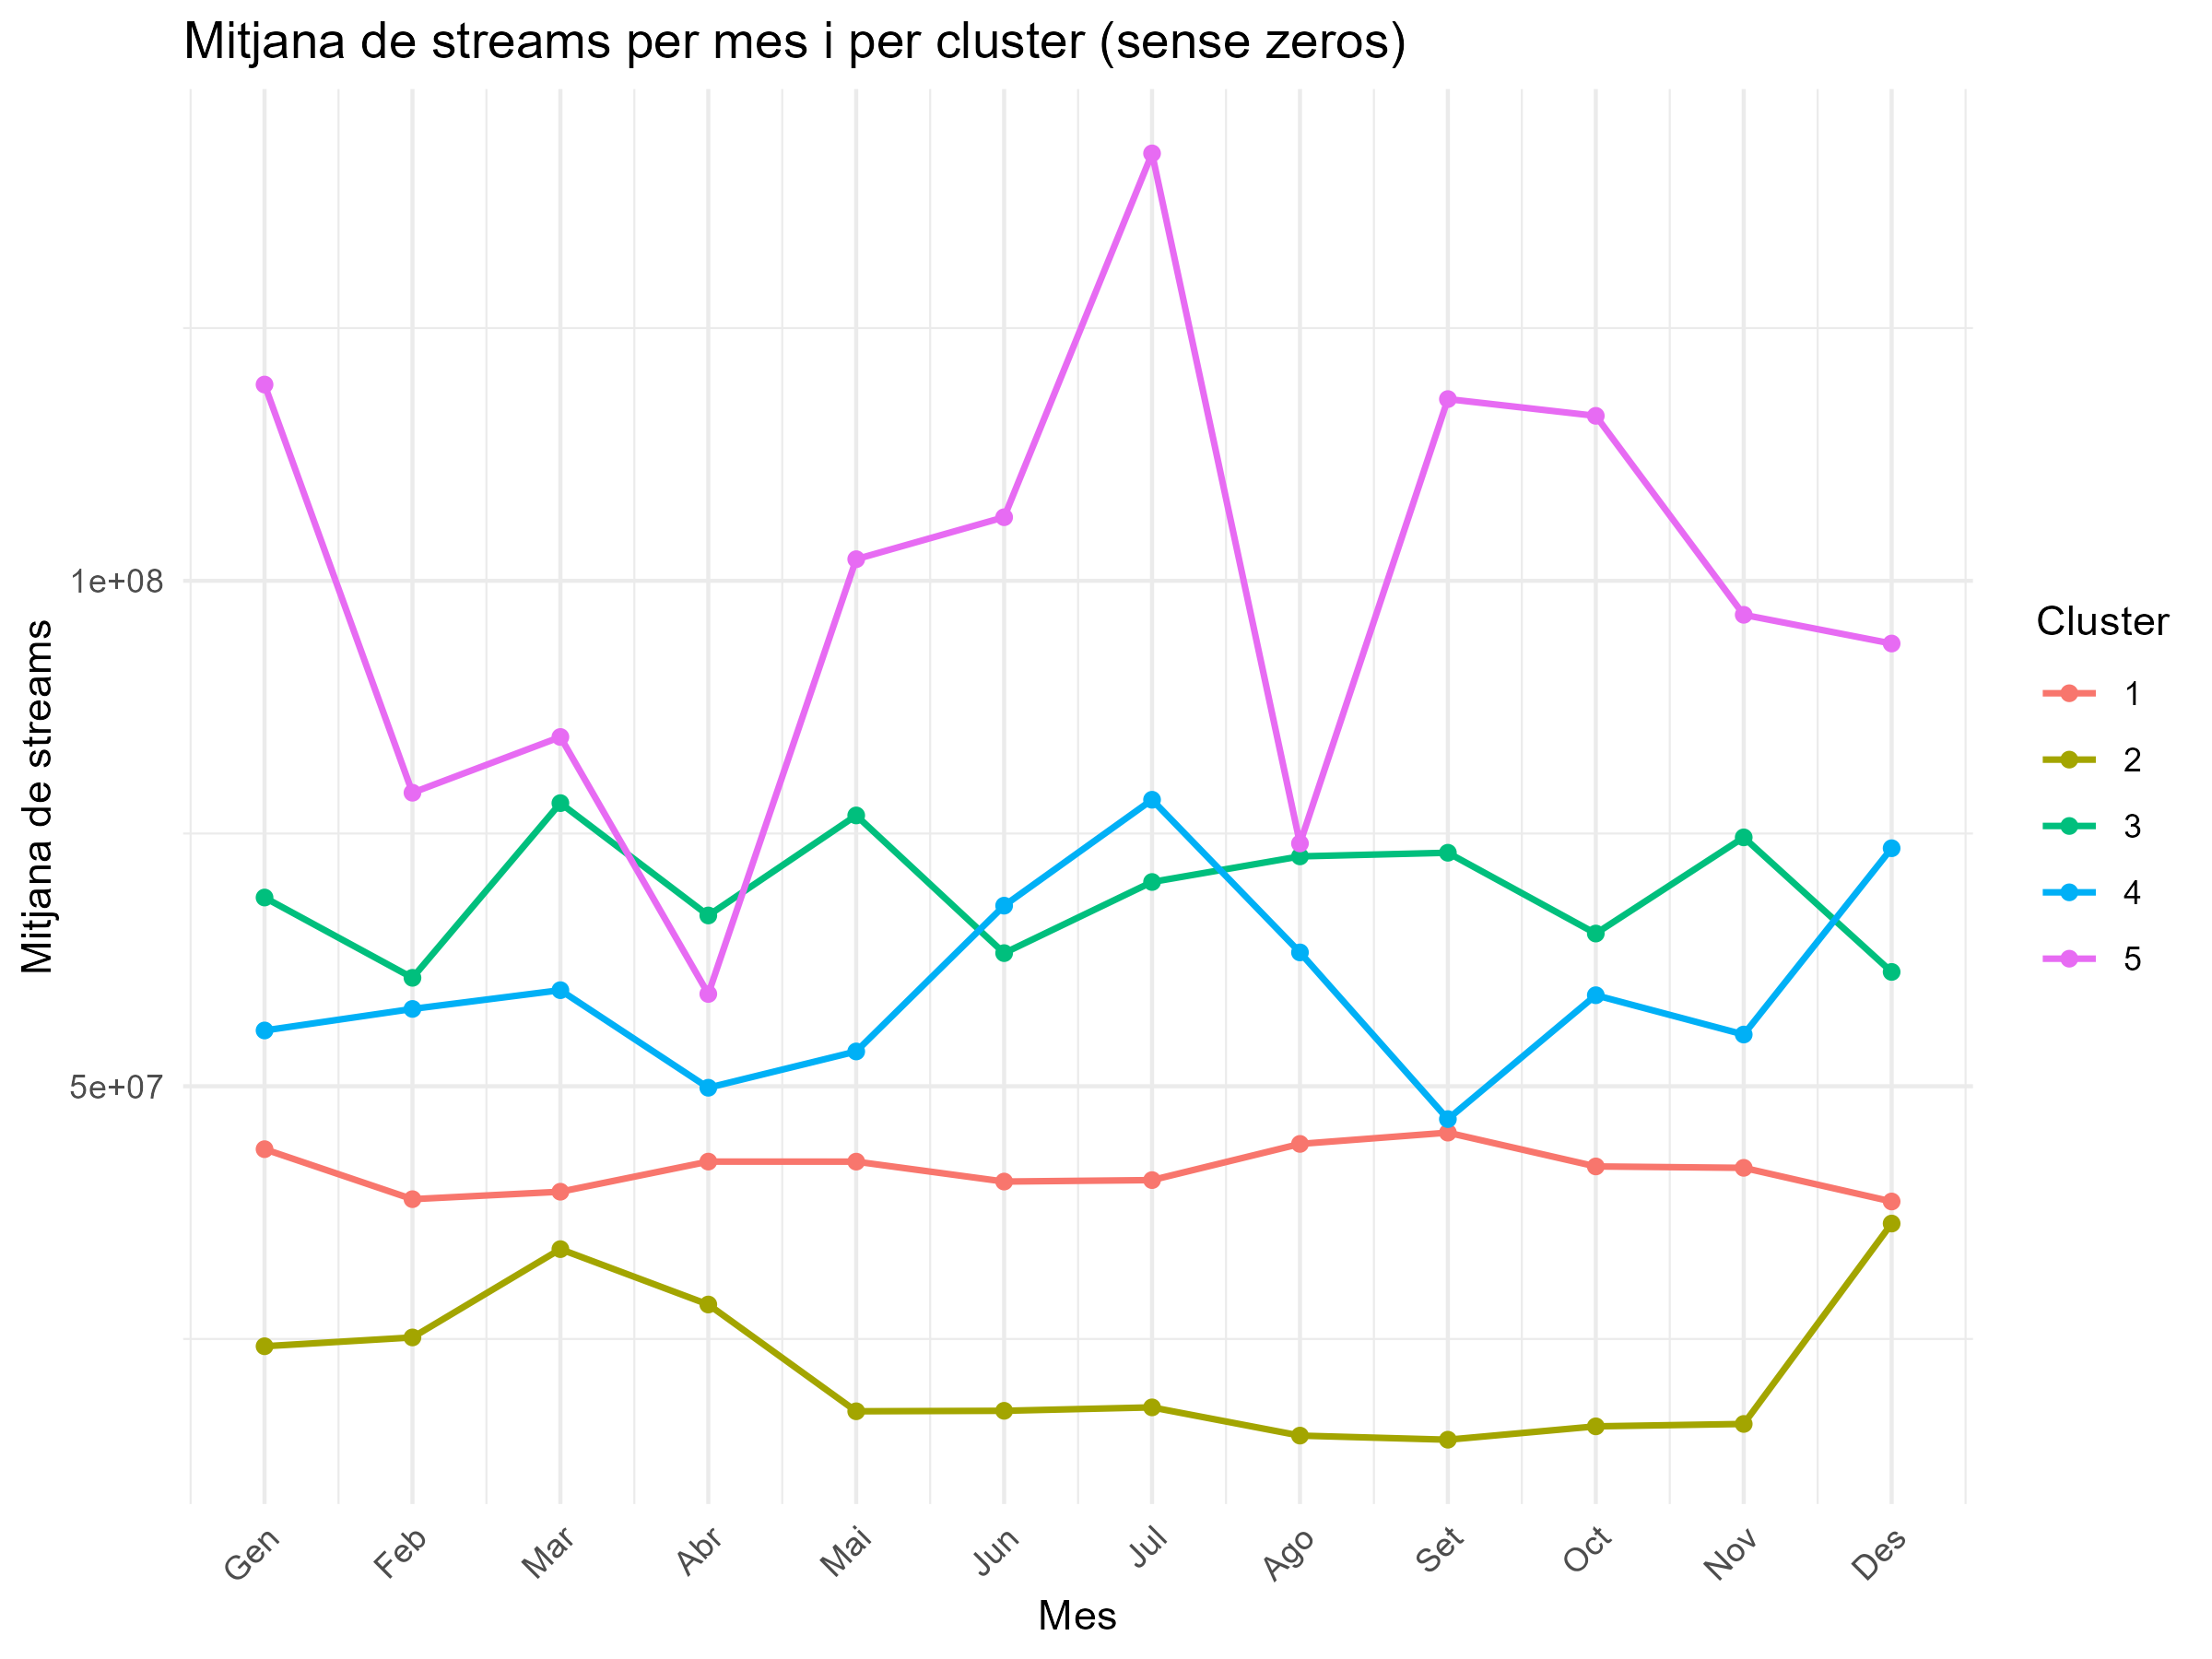
\includegraphics[width=0.8\textwidth]{Images/4_clustering/time_series/evol_streams_per_mes_i_cluster_no_0.png}
    \caption{Gràfic amb l'evolució de la mitjana de streams (sense considerar quan el valor és zero) de cada clúster en funció dels mesos}
    \label{fig:TS_evol_streams_per_mes_i_cluster_no_zeros}
\end{figure}

Amb tot el que s'ha vist, les conclusions són similars a les que s'han mencionat en l'anàlisi inicial. S'ha de tenir en compte que realizar un \textit{profiling} d'aquests clústers no és especialment fàcil, ja que s'han realitzat només tenint en compte el component temporal de streams en la base de dades, ignorant totes les altres variables.

Resumidament, es poden concloure les següents descripcions pels 5 clústers:
\begin{itemize}
    \item \textbf{Clúster 1:} Cançons poc populars i amb una durada no gaire sostinguda al llarg dels mesos.
    
    \item \textbf{Clúster 2:} El grup amb les cançons generalment menys populars i espontànies, tot i que amb alguns hits puntuals al desembre, que s'ha analitzat i, curiosament, no corresponen a cançons de nadal. Sembla contenir les cançons finals no tant populars del clúster 3.
    
    \item \textbf{Clúster 3:} Les cançons generalment més populars, sense ser les més antigues ni les més recents, i bastant sostingudes al llarg dels mesos en el top 40.
    
    \item \textbf{Clúster 4:} Cançons una mica menys populars que en el grup 3 i menys sostingudes, probablement perquè es concentren en els primers anys de la base de dades. Semblen ser les cançons inicials que manquen al clúster 3.
    
    \item \textbf{Clúster 5:} Les cançons més populars, més sostingudes al llarg dels mesos i que encara es trobaven presents al final del registre. Semblen ser les cançons populars finals que manquen al clúster 3.
\end{itemize}

Cal mencionar que l'existència dels clústers 4 i 5 pot ser deguda a que es troben en els inicis/finals dels mesos comptabilitzats a la base de dades, de manera que la seva sèrie temporal probablement té una forma especial (retallada pels extrems) que ha provocat que la distància DTW els separi, resultant en els dos grups amb menys cançons (només 40 i 8).

A més, també es pot afegir que en la figura \ref{fig:TS_dendrograma_colors} es confirma que els clústers 1 i 2 són els més similars, la qual cosa es podia preveure degut a la poca quantitat de streams que comparteixen.
